\documentclass{Control/UPV_control/UPV_utils/common/hap}
%\documentclass{common/hap}
\usepackage[utf8]{inputenc}
\usepackage[english]{babel}
\usepackage{listings}  % write xml code and other source codes
\usepackage{url}
\usepackage{amsmath}
\usepackage{paralist}  % Import compactenum class
\usepackage{color}
\usepackage[usenames,dvipsnames]{xcolor}
\usepackage{theorem}
\usepackage{amsfonts}
\usepackage{amssymb}
\usepackage{amsmath}
\usepackage{bm}

\usepackage{hyperref}
\usepackage{graphicx}
\usepackage{ifthen}
\newcommand{\mytextcite}[1]{\citet{#1}}
\newcommand{\myparencite}[1]{\citep{#1}}


% redefining chapters and sections


\newcommand{\customHeader}[2]{    
    \ifcase#1
       %This is case 0.
       \section{#2}
    \or
       %This is case 1.
       \subsection{#2}
    \or
       %This is case 2.
       \subsubsection{#2}
    \or
        % This is case 3
        \paragraph{#2}
    \else
        {\color{red} HEADER PROBLEM. LEVELS 0 to 2}
       %This is the default case.
    \fi
}


\newcommand{\headerName}[0]{Section} 
% \headerName exists so that I can write phrases like:
% "As seen in \headerName \ref{some label}"
\newcommand{\WARNING}[1]{
\colorbox{pink}{#1}
 }
\newcommand{\TODO}[0]{\WARNING{TODO}}
\newcommand{\todo}[1]{\WARNING{TODO: #1}}

\colorlet{body}{black!80!white}
\newcommand{\cvtag}[1]{%
  \tikz[baseline]\node[anchor=base,draw=body!30,rounded corners,inner xsep=1ex,inner ysep =0.75ex,text height=1.5ex,text depth=.25ex]{#1};
}

\newcommand{\putInBox}[1]{
\begin{tcolorbox}[colback=mylightblue,colframe=gray!50!black] 
#1
\end{tcolorbox}

}


\definecolor{mylightblue}{RGB}{207,226,243}
\definecolor{mylightyellow}{RGB}{252,229,205}


\newcommand{\appendixName}[0]{Appendix{}}

\newcommand{\INRAE}[0]{INRAE}
\newcommand{\MAIAGE}[0]{MaiAGE}
\newcommand{\PESV}[0]{PESV}
\newcommand{\VSI}[0]{VSI}
\newcommand{\bibliome}[0]{Bibliome}
\newcommand{\textclassification}[0]{Text Classification}
\newcommand{\tokenization}[0]{Tokenization}
\newcommand{\wordpiece}[0]{Word Piece}
\newcommand{\bpe}[0]{Byte-Pair Encoding}
\newcommand{\finetuning}[0]{Fine-tuning}
\newcommand{\PET}[0]{PET}



\newcommand{\fOne}[0]{\ensuremath{F_1}}
\newcommand{\fTwo}[0]{\ensuremath{F_2}}
\newcommand{\fBeta}[0]{\ensuremath{F_\beta}}
\newcommand{\auc}[0]{AUC}

\newcommand{\contentType}[0]{Content Source}

\newcommand{\trafilaturaTitle}[0]{Title}
\newcommand{\trafilaturaAbstract}[0]{Abstract}
\newcommand{\trafilaturaFulltext}[0]{Full text}
\newcommand{\translationTitle}[0]{Translated Title}
\newcommand{\trafilatura}[0]{Trafilatura}

\newcommand{\keyphrases}[0]{Phrases with Keywords}

\newcommand{\keyphrasesAbstractOnly}[0]{Phrases with Keywords (Abstract)}
\newcommand{\keyphrasesAbstractOC}[0]{Phrases with Keywords + O.C (Abstract)}

\newcommand{\keyphrasesFulltextOnly}[0]{Phrases with Keywords (Full text)}
\newcommand{\keyphrasesFulltextOC}[0]{Phrases with Keywords + O.C (Full text)}


\newcommand{\sanbaTitle}[0]{Title}
\newcommand{\sanbaAbstract}[0]{Abstract}

\newcommand{\sanba}[0]{Sanba}
\newcommand{\BERT}[0]{BERT}

\newcommand{\balanced}[0]{Balanced \finetuning{}}
\newcommand{\unbalanced}[0]{Unbalanced \finetuning{}}
\newcommand{\petFifty}[0]{PET 50}
\newcommand{\petOneHundred}[0]{PET 100}
\newcommand{\petTwoHundred}[0]{PET 200}
\newcommand{\petFiveHundred}[0]{PET 500}
\newcommand{\petThousand}[0]{PET 1000}


\newcommand{\bertbase}[0]{BERT-base}
\newcommand{\bertmultilingual}[0]{mBERT}
\newcommand{\bertbiolinkbert}[0]{Bio-Link-BERT}
\newcommand{\bertscibert}[0]{SciBERT}
\newcommand{\bertroberta}[0]{RoBERTa-base}
\newcommand{\bertxlmroberta}[0]{XLM-RoBERTa}

\newcommand{\neuralNetwork}[0]{Neural Network}

\newcommand{\mycoloredcell}[1]{
\cellcolor[rgb]{\fpeval{1-#1}, \fpeval{#1}, 0} \fpeval{round(100*#1, 2)} \%
}

\newcommand{\toPercentage}[1]{\fpeval{round(100*#1, 2)} \%}


%%% Colored table

\newcommand{\coloredTable}[1]{

\centering
\resizebox{\paperwidth}{!}{
\csvreader[
    tabular=|p{4cm}|*{7}{c|}p{4cm}|,
    table head=\hline %\rowcolor{gray!20} 
    \contentType{} & \unbalanced{} & \balanced{} & \petFifty{} & \petOneHundred & \petTwoHundred{} & \petFiveHundred{} & \petThousand{} & \contentType{}  \\ \hline,
    %late after line=\\ \hline
    late after line=\\, late after last line=\\\hline
    ]%
    {#1}{}%
    {
    \csvcolii
    & \cellcolor[rgb]{\fpeval{(1-\csvcoliii)}, \fpeval{\csvcoliii}, 0} \fpeval{round(100*\csvcoliii, 2)}\% 
    & \cellcolor[rgb]{\fpeval{1-\csvcoliv}, \fpeval{\csvcoliv}, 0} \fpeval{round(100*\csvcoliv, 2)}\% 
    & \cellcolor[rgb]{\fpeval{1-\csvcolv}, \fpeval{\csvcolv}, 0} \fpeval{round(100*\csvcolv, 2)}\%
    & \cellcolor[rgb]{\fpeval{1-\csvcolvi}, \fpeval{\csvcolvi}, 0} \fpeval{round(100*\csvcolvi, 2)}\%
    & \cellcolor[rgb]{\fpeval{1-\csvcolvii}, \fpeval{\csvcolvii}, 0} \fpeval{round(100*\csvcolvii, 2)}\% 
    & \cellcolor[rgb]{\fpeval{1-\csvcolviii}, \fpeval{\csvcolviii}, 0} \fpeval{round(100*\csvcolviii, 2)}\%
    & \cellcolor[rgb]{\fpeval{1-\csvcolix}, \fpeval{\csvcolix}, 0} \fpeval{round(100*\csvcolix{}, 2)}\%
    & \cellcolor{white} \csvcolii
    }
}


}


%%% Split Statistics table

\newcommand{\splitsFinetuningTable}[1]{

    \centering
    \resizebox{\textwidth}{!}{
    \csvreader[
        tabular=|p{4cm}|*{9}{c|},
        table head=\hline
        \contentType{}
        & Train-Size
        & Positives
        & Negatives
        & Dev-Size
        & Positives
        & Negatives
        & Test-Size
        & Positives
        & Negatives
        \\ \hline,
        late after line=\\, 
        late after last line=\\\hline
        ]%
        {#1}{}%
        {
        \csvcolii
        & \csvcoliii
        & \csvcoliv
        & \csvcolv
        & \csvcolvi
        & \csvcolvii
        & \csvcolviii
        & \csvcolix
        & \csvcolx
        & \csvcolxi
        }
    }
}

\newcommand{\splitsPetTable}[1]{

    \centering
    \resizebox{\textwidth}{!}{
    \csvreader[
        tabular=|p{4cm}|*{10}{c|},
        table head=\hline
        \contentType{}
        & Train-Size
        & Positives
        & Negatives
        & Dev-Size
        & Positives
        & Negatives
        & Test-Size
        & Positives
        & Negatives
        & Unlabeled
        \\ \hline,
        late after line=\\, 
        late after last line=\\\hline
        ]%
        {#1}{}%
        {
        \csvcolii
        & \csvcoliii
        & \csvcoliv
        & \csvcolv
        & \csvcolvi
        & \csvcolvii
        & \csvcolviii
        & \csvcolix
        & \csvcolx
        & \csvcolxi
        & \csvcolxii
        }
    }
}




%%% Epchs Statistics table

\newcommand{\epochTable}[1]{

    \centering
    \resizebox{\textwidth}{!}{
    \csvreader[
        tabular=|p{4cm}|*{8}{c|},
        table head=\hline
        Model 
        & \trafilaturaTitle{}
        & \trafilaturaAbstract{}
        & \trafilaturaFulltext{}
        & \translationTitle{}
        & \keyphrasesAbstractOnly{}
        & \keyphrasesAbstractOC{}
        & \keyphrasesFulltextOnly{}
        & \keyphrasesFulltextOC{}
        \\ \hline,
        late after line=\\, 
        late after last line=\\\hline
        ]%
        {#1}{}%
        {
        \csvcoli
        & \csvcolii
        & \csvcoliii
        & \csvcoliv
        & \csvcolv
        & \csvcolvi
        & \csvcolvii
        & \csvcolviii
        & \csvcolix
        }
    }
}


\setlength{\headheight}{15.2pt}

%% WARNING!: use 'pdflatex' command to compile this file.

%% Put here the title of the work
\def\Title{Long Title\\that can Span Multiple Lines\\}

%% The ``short'' title of the work.
%% This will be put in the header of the document. Let it be \Title in the case
%% is short enough
\def\ShortTitle{Short Title}

%% Put here the author
\def\Authors{Luis Antonio VASQUEZ REINA}

%% Put here the tutor
\def\Tutor{
\href{https://ragerri.github.io/}{Rodrigo AGERRI} (\href{https://www.ehu.eus/es/web/informatika-fakultatea}{Informatics Faculty  at UPV-EHU })\\
\href{https://maiage.inrae.fr/fr/robert-bossy}{Robert BOSSY} (\href{https://maiage.inrae.fr/}{
%Math\'ematiques et Informatique Appliqu\'ees du G\'enome \`{a} l'Environnement (MaIAGE)}
MaIAGE} Research Group at \href{https://inrae.fr/}{INRAE}
)\\
\href{https://members.loria.fr/mcouceiro/}{Miguel COUCEIRO} (\href{https://idmc.univ-lorraine.fr/}{IDMC Institute} at \href{https://www.univ-lorraine.fr/}{Universit\'e de Lorraine})\\

}

%% The date
\def\Date{August 2023}
%% Abstract
\def\AbstractEusk{Abstract in Basque.}

\def\AbstractEng{Abstract in English.}

%%%%%%%% Don't touch the following lines
%%%%%%% Taken from MEANING style
\newcommand {\deltitle}{ \LARGE {\textbf{\Title}}}
\DocTitle{\ShortTitle}
\DocDate{\Date}

\addto\captionsbasque{%
  \renewcommand{\contentsname}{Contents}%
  \renewcommand{\listfigurename}{List of figures}%
  \renewcommand{\listtablename}{List of tables}%
}

\begin{document}
\begin{titlepage}
{ \center
  \begin{minipage}{\textwidth}
    \centering
    
\includegraphics[height=3cm]{Control/UPV_control/UPV_utils/common/ehuLogo.png}
    %
\includegraphics[height=3cm]{common/ehuLogo}
  \end{minipage}
}\\[15pt]

\begin{minipage}[t][4cm][c]{\textwidth}
  \center
  \deltitle
{ \large \textbf{Author:} \Authors }\\
{ \large \textbf{Advisors:} \Tutor}\ \\
%\vspace{-8pt}
\vspace{0.5cm}
\end{minipage}\\
\begin{center}
%  \centering \textcolor{blue}{\Huge \textbf{hap/lap}}
  \resizebox{0.7\linewidth}{!}{ \textcolor{blue}{\texttt{hap/lap}}}
\end{center}

\vspace{0.3cm}
\begin{center}
  Hizkuntzaren Azterketa eta Prozesamendua\\Language Analysis and Processing\\
\vspace{0.3cm}
  {\Large \textbf{Final Thesis}}
\end{center}
\vspace{0.1cm}
\begin{center}
  \Date
\end{center}
\HRule \\[0.3cm]
{ \textbf{Departments}: Computer Systems and Languages, Computational Architectures and Technologies, Computational Science and Artificial Intelligence, Basque Language and Communication, Communications Engineer. }\\[0.3cm]
 \HRule \\[0.5cm]

\end{titlepage}
\renewcommand{\thepage}{\roman{page}}
\cleardoublepage
\newpage
\begin{center}
  \vspace*{\fill}
  \begin{minipage}{1.0\textwidth}
    \begin{center}
     \textbf{Laburpena}\\
     \AbstractEusk
    \end{center}
    \begin{center}
     \textbf{Abstract}\\
     \AbstractEng
    \end{center}
  \end{minipage}
  \vspace*{\fill}
\end{center}
\cleardoublepage
\tableofcontents
\cleardoublepage
\listoffigures
\cleardoublepage
\listoftables
\cleardoublepage
\setcounter{page}{1}
\renewcommand{\thepage}{\arabic{page}}
%%%%%%%%%%%%%%%%%%%%%%%%%%%%%%%%%%%%%%%%%%%%%%%%%%%%%%%%

%%%%%%% Don't touch the following lines
%%%%%%% Taken from MEANING style
\newcommand {\deltitle}{ \LARGE {\textbf{\Title}}}
\DocTitle{\ShortTitle}
\DocDate{\Date}

\addto\captionsbasque{%
  \renewcommand{\contentsname}{Contents}%
  \renewcommand{\listfigurename}{List of figures}%
  \renewcommand{\listtablename}{List of tables}%
}

\begin{document}
\begin{titlepage}
{ \center
  \begin{minipage}{\textwidth}
    \centering
    
\includegraphics[height=3cm]{Control/UPV_control/UPV_utils/common/ehuLogo.png}
    %
\includegraphics[height=3cm]{common/ehuLogo}
  \end{minipage}
}\\[15pt]

\begin{minipage}[t][4cm][c]{\textwidth}
  \center
  \deltitle
{ \large \textbf{Author:} \Authors }\\
{ \large \textbf{Advisors:} \Tutor}\ \\
%\vspace{-8pt}
\vspace{0.5cm}
\end{minipage}\\
\begin{center}
%  \centering \textcolor{blue}{\Huge \textbf{hap/lap}}
  \resizebox{0.7\linewidth}{!}{ \textcolor{blue}{\texttt{hap/lap}}}
\end{center}

\vspace{0.3cm}
\begin{center}
  Hizkuntzaren Azterketa eta Prozesamendua\\Language Analysis and Processing\\
\vspace{0.3cm}
  {\Large \textbf{Final Thesis}}
\end{center}
\vspace{0.1cm}
\begin{center}
  \Date
\end{center}
\HRule \\[0.3cm]
{ \textbf{Departments}: Computer Systems and Languages, Computational Architectures and Technologies, Computational Science and Artificial Intelligence, Basque Language and Communication, Communications Engineer. }\\[0.3cm]
 \HRule \\[0.5cm]

\end{titlepage}
\renewcommand{\thepage}{\roman{page}}
\cleardoublepage
\newpage
\begin{center}
  \vspace*{\fill}
  \begin{minipage}{1.0\textwidth}
    \begin{center}
     \textbf{Laburpena}\\
     \AbstractEusk
    \end{center}
    \begin{center}
     \textbf{Abstract}\\
     \AbstractEng
    \end{center}
  \end{minipage}
  \vspace*{\fill}
\end{center}
\cleardoublepage
\tableofcontents
\cleardoublepage
\listoffigures
\cleardoublepage
\listoftables
\cleardoublepage
\setcounter{page}{1}
\renewcommand{\thepage}{\arabic{page}}
%%%%%%%%%%%%%%%%%%%%%%%%%%%%%%%%%%%%%%%%%%%%%%%%%%%%%%%%



%% file for managing the content of the thesis


%\chapter{Introduction}
\customHeader{0}{Introduction}
\label{Introduction}

\customHeader{1}{Background and Motivation}
\label{01_2_background_and_motivation}

\customHeader{2}{Hosting Institution : \INRAE{} Laboratory}
\label{01_2_1_INRAE}

\href{https://www.inrae.fr/}{\INRAE{} }\footnote{\url{https://www.inrae.fr/}}  (\emph{Institut National de Recherche} \emph{pour l'Agriculture, l'Alimentation et l'Environnement}) is a French research institute dedicated to agriculture, food, and the environment. 

\INRAE{} conducts scientific research and innovation activities to address various challenges related to sustainable agriculture, food production, and environmental conservation. Its research efforts span a wide range of disciplines, including agronomy, biology, ecology, genetics, forestry, hydrology, and social sciences.

Through its multidisciplinary approach and emphasis on sustainability, \INRAE{} plays a crucial role in driving scientific progress, innovation, and policy development in France and beyond, with the ultimate aim of ensuring sustainable and resilient agricultural and environmental systems.

Within \INRAE{}, the Mathematics and Numerics division (\href{https://www.inrae.fr/departements/mathnum}{MathNum}\footnote{\url{https://www.inrae.fr/departements/mathnum}}) focuses on advancing research in various fields including applied mathematics, statistics, bioinformatics, \gls{ai}, and information technology. The division's research units engage in theoretical, methodological, and applied research. They actively collaborate with teams from different divisions within \INRAE{} and external organizations, fostering interdisciplinary partnerships. \href{https://maiage.mathnum.inrae.fr}{\MAIAGE{}}\footnote{\url{https://maiage.mathnum.inrae.fr}}, one of these research units, is associated to the Paris-Saclay University, and brings together mathematicians, computer scientists, bioinformaticians, and biologists to address challenges in the fields of biology, agronomy, and ecology. This project was carried out with alongside the  \href{https://maiage.mathnum.inrae.fr/fr/bibliome}{\bibliome{}}\footnote{\url{https://maiage.mathnum.inrae.fr/fr/bibliome}} team, which specializes in the advancement of \gls{nlp} and \gls{ml} techniques tailored for textual data within the fields of biology and agronomy.  



\newpage
\customHeader{0}{Background}
\label{02_background}

This \headerName{} introduces the conceptual tools necessary to understand our project, our methodology, and our results.



\customHeader{1}{Text Classification}
\label{02_text_classification}

Text classification, is a fundamental task in \gls{nlp} that involves automatically assigning predefined categories or labels to text documents based on their content. The goal of text classification is to develop computational models that can accurately classify text documents into predefined categories, enabling automated organization, retrieval, and analysis of large volumes of textual data.

Formally, given a set $V$ called the \emph{Vocabulary}, and a set $C$ of \emph{categories}, a \emph{\textclassification{} System} is a function 
$$f: V^*\times C \mapsto \{ \texttt{True}, \texttt{False} \}$$

where $V^*$ is the set of finite sequences of elements of $V$, that is, the set of \emph{documents}. 
While the general definition of document classification accommodates multi-label classification scenarios, the specific focus of this project is on \emph{Binary \textclassification{}}. In this particular case, the classification task involves assigning documents to one of two mutually exclusive categories \myparencite{Shen2009_text_classification_formal_definition}.

In the context of document classification, the fundamental objective is to leverage a training set, comprising a collection of training documents $(d_i, c_i)$, and employ a learning method or algorithm to derive a \emph{Classifier} $\gamma$. The primary purpose of this classifier is to establish a mapping from documents to classes, denoted as 
$$\gamma : V^* \mapsto \{1, 0\}$$

\customHeader{1}{\neuralNetwork{}s}
\label{02_neural_networks}




In this section, we present the fundamental concepts necessary for understanding \neuralNetwork{}s, drawing on the Open Access material from \mytextcite{deep_learning_introduction} and \mytextcite{wolfram_llm}.

\customHeader{2}{Motivating Example}
\label{02_nn_motivating_example}


To understand the rationale behind using \neuralNetwork{}s, let's consider a scenario where we aim to determine how the temperature and humidity of a place relate to the perceived temperature by living beings, such as humans. In other words, given these two metrics across various locations, our goal is to forecast the felt temperature or Heat Index for each site. A simplified version of the model from \mytextcite{heat_index}, can provide us with an equation for the Heat Index ($HI$).

\begin{align*}
    HI &= w_{Temp} T + w_{Hum} H + c
\end{align*}


The main idea behind this model is that the heat index, our \emph{target}, can be calculated as a weighted sum of the temperature $T$ and the humidity $H$. The influence of $T$ on the $HI$ is given by $w_{Temp}$ and that of $H$ by $w_{Hum}$, and we correct by a constant value $c$. 

In this model, $H$ and $T$ are termed the \emph{features} of a location, serving as its defining characteristics. Essentially, locations with identical features will yield the same output. The terms $w_{Temp}$ and $w_{Hum}$ are referred to as \emph{weights} or \emph{parameters}. They signify the relevance of the features to the model. For instance, if $w_{Hum}$ is zero, the $HI$ would solely be influenced by $T$. Additionally, $c$ is labeled as the \emph{bias} or \emph{offset}, representing the output value when the features are null. The equation's right-hand side, $w_{Temp} T + w_{Hum} H + c$, is recognized as the model's \emph{output} or \emph{prediction}.


In practice, the values for the weights and bias of this model have been determined to be:
\begin{align*}
w_{Temp} & = 1.1\
w_{Hum} &= 0.047 \
c &= -10.3
\end{align*}

Yet, this basic representation has its limitations. Interestingly, by introducing an additional computational step, we can achieve more accurate results. Let's consider incorporating a minor squared term through the function $f(u) = u + 0.0002 u^2$. With this, our model evolves to:

\begin{align*}
HI &= f(w_{Temp} T + w_{Hum} H + c)
\end{align*}

In this enhanced model, $f$ is termed the \emph{activation function}. The model's prediction or output is derived by applying $f$ to the weighted sum. This added computation step allows for a more authentic representation of how living beings respond to significant shifts in temperature and humidity. 
In general, this kind of model allows us to use numerical features, to obtain a prediction for a variable of interest.

\customHeader{2}{Neurons}
\label{02_nn_neurons}




When dealing with increasingly complex phenomena, it becomes challenging to explicitly define the parameters for a model. This necessitates a broader approach. In the realm of Machine Learning, the concept of \emph{neurons} serves as a generalization of the model described earlier.

\input{Figures/02/Basic_neuron}

Imagine a model where the inputs encompass $n$ distinct features, represented as $(x_1, x_2,\ldots,x_n)$. The diagram depicted in Figure \ref{fig:02_neuron} represents the following equation:

\begin{align*}
z &= f(w_1 x_1 + w_2 x_2 + \ldots + w_d x_d + b)
\end{align*}

Here, $w_1, w_2,\ldots,w_n$ denote the weights, $b$ signifies the bias, $f$ is the activation function, and $z$ stands for the prediction.

One of the main insights in \gls{ml} is that one does not need to manually define the parameters $(w_1, w_2,\ldots,w_n,b)$ for this kind of model.
Instead, with ample data comprising input features and observed target values, it's feasible to determine the best parameter values. This ensures the model's predictions closely align with the observed target values. Once established, this model can be applied to new data. The process of finding the optimal parameters is called \emph{training}.

In order to find the optimal parameters, we first need to decide how to produce our final predictions, how to measure how well the model is performing, and how to update the model's parameters.


\customHeader{2}{Activation functions}
\label{02_nn_activation_functions}


The method used to derive our final predictions is contingent on the specific problem to be addressed. Various activation functions cater to different problems. For instance, in \emph{regression}, where our objective is to compute a continuous quantity,  like in the example in \headerName{} \ref{02_nn_motivating_example}, we may handle values that can range from extremely small to exceedingly large. On the other hand, classification tasks aim to predict a categorical label, either by taking a final decision or by producing probabilities for each category.


Table \ref{tab:02_nn_common_activation_functions} and Figure \ref{fig:02_nn_common_activation_functions} enumerate some of the most common activation functions.

\input{Tables/02/Activation_functions}

\begin{figure}[ht]
    \centering
    \subfigure[Identity]{
        \begin{adjustbox}{max height=0.07\textheight}
            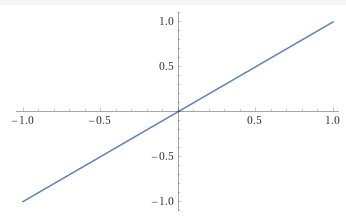
\includegraphics[width=0.45\textwidth]{Figures/02/Activation_functions/02_Identity.png}
        \end{adjustbox}
        
        %\label{fig:image1}
    }
    \hfill
    \subfigure[ReLU]{
        \begin{adjustbox}{max height=0.07\textheight}
            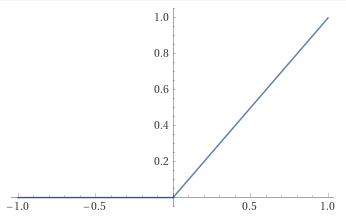
\includegraphics[width=0.45\textwidth]{Figures/02/Activation_functions/02_Relu.png}
        \end{adjustbox}
        
        %\label{fig:image2}
    }
    \hfill
    \subfigure[Sigmoid]{
        \begin{adjustbox}{max height=0.07\textheight}
            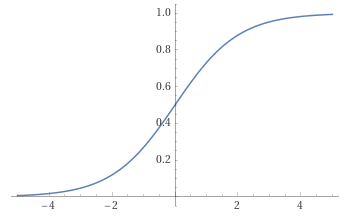
\includegraphics[width=0.45\textwidth]{Figures/02/Activation_functions/02_sigmoid.png}
        \end{adjustbox}
        
        %\label{fig:image1}
    }
    \hfill
    \subfigure[Tanh]{
        \begin{adjustbox}{max height=0.07\textheight}
            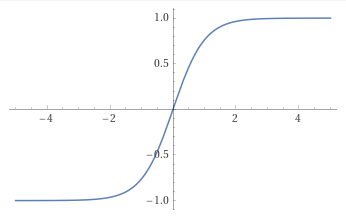
\includegraphics[width=0.45\textwidth]{Figures/02/Activation_functions/02_tanh.png}
        \end{adjustbox}
        
        %\label{fig:image2}
    }
    \caption{Common activation functions}
    \label{fig:02_nn_common_activation_functions}
\end{figure}





\customHeader{2}{Loss Functions}
\label{02_nn_loss_functions}


Loss functions quantify the deviation of predicted values from actual target values. The goal during training is to adjust the parameters to minimize this deviation. The process of inputting data into the neuron to compute the loss is termed the \emph{forward pass}.

For regression tasks, the squared error is frequently employed. It calculates the squared difference between the predicted and actual values:

\begin{equation}
loss_{SE}(x,w,b) = \dfrac{1}{2} (z_{pred}(x,w,b)-z_{real})^2
\end{equation}

where $z_{pred} = f(xw+b)$.

In classification tasks, the \emph{cross-entropy} loss is common. The essence of cross-entropy is to maximize the model's confidence in its category assignments\footnote{Deducing the formula for Cross-Entropy is outside the scope of this work}. Given features $x = x_1, x_2, \ldots, x_n$ and predicted probabilities $p_1, p_2, \ldots, p_k$ for categories $c_1, c_2, \ldots, c_k$, and representing actual categories as $(q_1, q_2, \ldots, q_k)$ where $q_j =1 $ for category $j$ and $q_j = 0$ otherwise, cross entropy is:

\begin{equation}
loss_{CE}(x,w,b) = - \sum_{j} q_{j}(x) \log{(p_{j}(x,w,b))}
\end{equation}

For datasets with uneven category distribution, or \emph{unbalanced} datasets, a modified version called \emph{weighted cross-entropy} can be used. It adjusts the cross-entropy based on category representation. If category $j$ has a weight of $r_j$, then:

\begin{equation}
loss_{WCE}(x,w,b) = - \sum_{j} r_j q_{j}(x) \log{(p_{j}(x,w,b))}
\end{equation}


\customHeader{2}{Backpropagation}
\label{02_nn_loss_back_propagation}

After measuring the performance of a neuron through the loss, our aim is to adjust its parameters to reduce this loss. The process of \emph{updating} the weights to achieve this reduction is termed \emph{backpropagation}. A common  optimization technique to achieve this is \emph{gradient descent}. For illustrative purposes, let's assume that the neuron has just one weight, and thus, there's just one weight influencing the loss (as depicted in Figure \ref{fig:02_nn_gradient_descent}). The key insight is that moving against the slope of the loss curve brings us closer to its minimum. This slope is the derivative or the \emph{gradient} of the loss function. Through several iterative steps, updating the weight each time, we eventually reach the ideal weight that minimizes the loss.

\begin{figure}
\centering
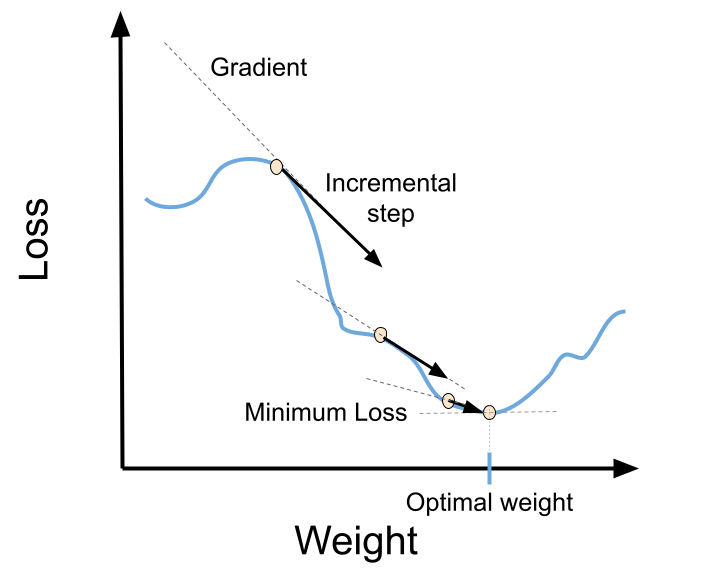
\includegraphics[width=0.5\textwidth]{Figures/02/02_gradient_descent.png}
\caption{Gradient descent illustration}
\label{fig:02_nn_gradient_descent}
\end{figure}

Having identified the direction of adjustment, it's also crucial to regulate the magnitude of this adjustment. This is achieved using the \emph{learning rate} $\eta$, which moderates the gradient's impact on weight updates. That is, our weight updating process is calculated in the following way:

\begin{align}
w_{new} = w_{old} - \eta \nabla loss(x, w_{old}) \label{eq:02_nn_gradient_descent}
\end{align}



% gradient descent
% learning rate
% loss optimization

\customHeader{2}{Training}
\label{02_nn_training}



Up to this point, we've discussed using just one feature vector as input for a neuron. But for a comprehensive representation of our task, multiple examples are essential. This means, for effective training, we require multiple data points, or in other words, a \emph{Dataset} comprising both features and their corresponding observed target values $(x,z_{real})$. If our Dataset $D$ contains $N$ items, our goal becomes minimizing the \emph{average} loss across the dataset:

\begin{equation}
Loss(w,b) = \dfrac{1}{N} \sum_{x\in D} loss(x,w,b)
\end{equation}

The entire process of executing the forward pass, determining the loss, and updating weights through backpropagation is termed an \emph{epoch} (as illustrated in Figure \ref{fig:02_nn_neuron_training}).

\begin{figure}
\centering
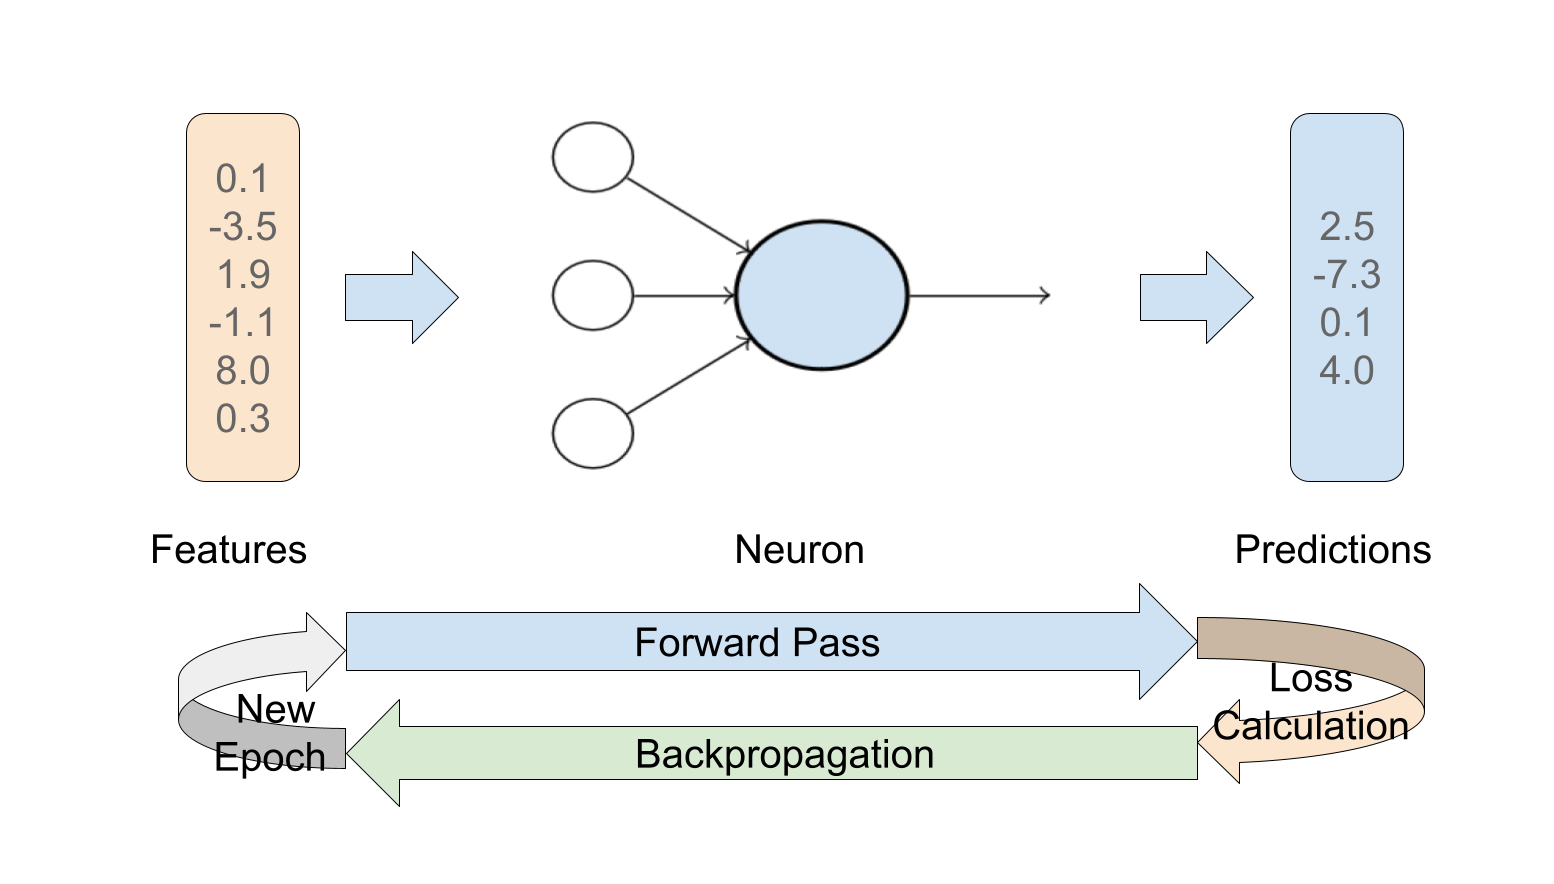
\includegraphics[width=0.75\textwidth]{Figures/02/02_neuron_training.png}
\caption{Neuron Training Process}
\label{fig:02_nn_neuron_training}
\end{figure}

In most cases, our computing resources might not possess the capacity to process the entire Dataset in one run. A common workaround is segmenting the Dataset into equally sized \emph{batches}. The forward pass and loss computation are then executed batch by batch until the entire dataset is covered. Subsequently, the losses from each batch are combined to determine the final loss, followed by backpropagation. Typical batch sizes include powers of 2: $2, 4, 8, 16, 32, 64, \ldots, 2^n, \ldots$

Often, a single epoch doesn't suffice to yield satisfactory outcomes. Hence, it's a standard practice to train a neuron over multiple epochs. With each epoch, the loss typically reduces (as depicted in Figure \ref{fig:02_nn_loss_evolution}).

\begin{figure}
    \centering
    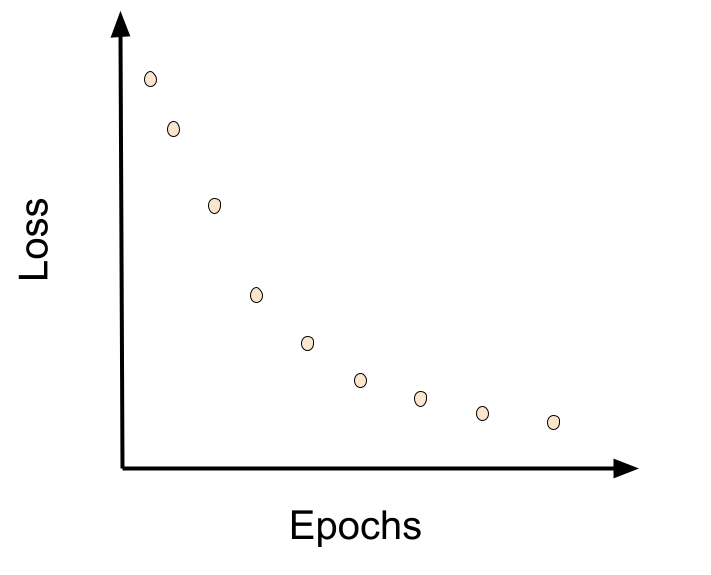
\includegraphics[width=0.5\textwidth]{Figures/02/02_loss_evolution.png}
    \caption{Evolution of loss during training}
    \label{fig:02_nn_loss_evolution}
\end{figure}

% batches
% epochs

\customHeader{2}{Overfitting }
\label{02_nn_overfitting}


As we progressively reduce our loss, we encounter a challenge. There are instances when the neuron will produce excellent predictions for the data it was trained on, but performs poorly on entirely new data, rendering the neuron useless for real-world applications. This issue is termed \emph{overfitting}.

A prevalent strategy to counteract overfitting is to \emph{divide} the dataset into three distinct portions:

\begin{enumerate}
\item The \emph{training} split, which constitutes a portion of the dataset dedicated to the core training processes, including the forward pass, loss evaluation, and crucially, backpropagation.
\item The \emph{development} split, a portion of the dataset designated for tracking potential overfitting. For this split, we execute the forward pass and compute the loss, and occasionally other metrics, but refrain from backpropagation. Recognizing the beginning of overfitting allows us to adjust our setup for the optimal number of epochs.
\item The \emph{test} split, a portion of the dataset reserved for assessing the efficacy of the chosen training setup, especially since this subset wasn't involved in its selection.
\end{enumerate}

When monitoring the trajectory of the loss across the training and development splits, a pattern emerges. After a specific number of epochs, the loss on the training split continues to drop, but the development split's loss starts to climb. This shift marks the beginning of overfitting (depicted in Figure \ref{fig:02_nn_split_loss_evolution}).

\begin{figure}
    \centering
    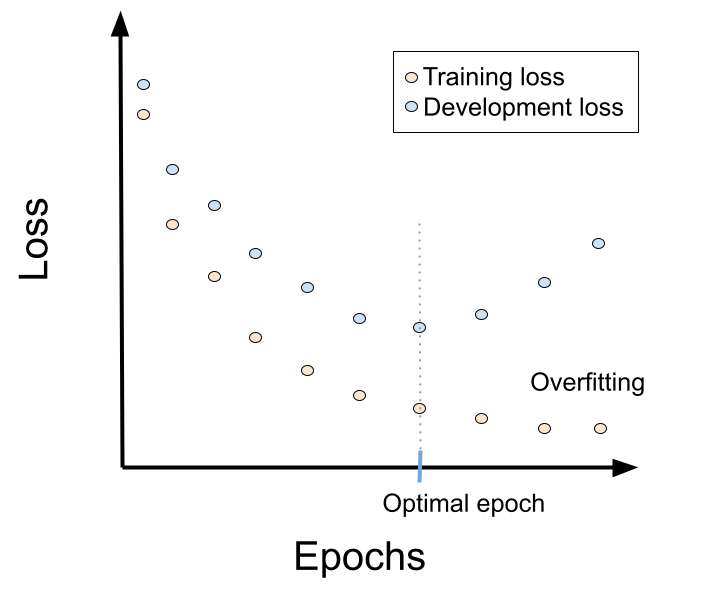
\includegraphics[width=0.5\textwidth]{Figures/02/02_split_loss_evolution.png}
    \caption{Evolution of loss on the training and development splits}
    \label{fig:02_nn_split_loss_evolution}
\end{figure}


% splits.
% plot for optimal epoch

\customHeader{2}{Optimizers }
\label{02_nn_optimizers}

% optimizers
We may generalize Gradient Descent (Equation \ref{eq:02_nn_gradient_descent}), by noticing that we only need to calculate some way to update our weights:

\begin{equation}
    w_{new} = w_{old} - \texttt{Update}(x, w_{old})
\end{equation}

Different optimization methods calculate the \texttt{Update} in different ways. Software implementations of these optimization methods are called \emph{optimizers}. Some common methods are listed in Table \ref{tab:02_nn_common_optimizers}, listed by increasing performance.

\input{Tables/02/Optimizers}


\customHeader{2}{Feed-Forward \neuralNetwork{}s}
\label{02_nn_ffnn}

As we have seen, an individual neuron may take several inputs to give an output, and this provides us with a model useful for some applications. 
One of the groundbreaking insights in \gls{ml} was the idea of linking neurons together. This involves using the output of one neuron as the input for others. By organizing neurons into \emph{linear layers} and interconnecting them, we create a \gls{ffnn} (Refer to Figure \ref{fig:02_nn_ffnn})\footnote{All diagrams of \neuralNetwork{} were made with the $NN-SVG$ tool by \mytextcite{drawing_nns}}.

\begin{figure}
    \centering
    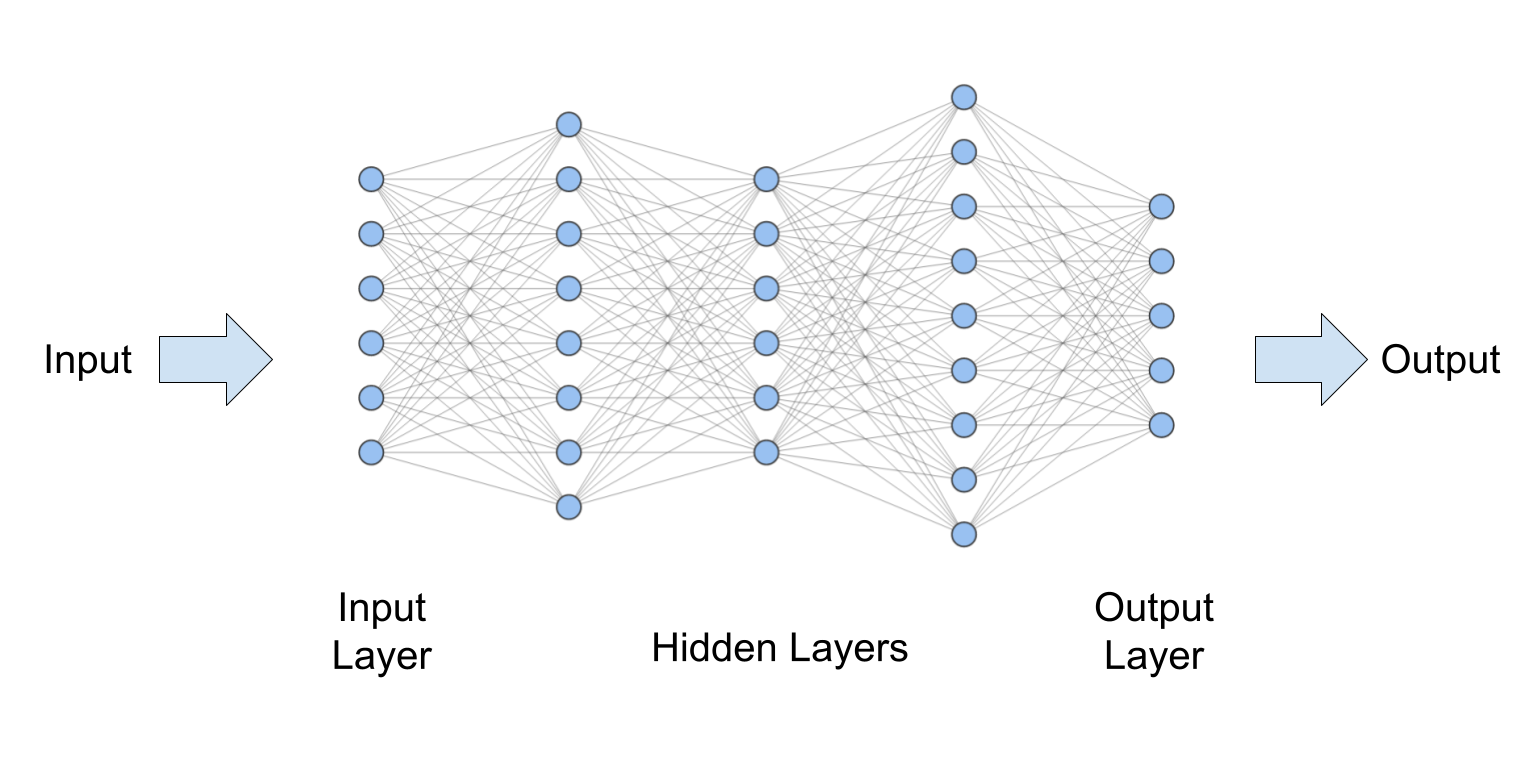
\includegraphics[width=0.75\textwidth]{Figures/02/02_FFNN.png}
    \caption{A Feed-Forward \neuralNetwork{}}
    \label{fig:02_nn_ffnn}
\end{figure}

When performing the forward pass, input features are fed into the \gls{ffnn} via the \emph{input layer}, they traverse through intermediate layers until they reach the \emph{output layer}.
As the \gls{ffnn} undergoes training, every intermediate layer crafts new features for the subsequent layers. 
This mechanism enables the \gls{ffnn} to \emph{learn} new representations for the data.
These in-between, or \emph{hidden}, features detect and leverage patterns from earlier features to determine the final output of the \neuralNetwork{}. A \neuralNetwork{} with just one hidden layer is termed \emph{shallow}, whereas those with several hidden layers are called \emph{deep}.

For classification tasks, the \gls{softmax} activation function is typically employed in the output layer since it yields a probability distribution across various categories. Such a layer is termed a \emph{\gls{softmax} layer} or a \emph{classification layer}. The inputs to this layer are often referred to as \emph{logits}. Given that we're working with probabilities, the objective is to minimize the cross-entropy loss between the predictions of the \neuralNetwork{} and the true labels.
(Refer to Figure \ref{fig:02_nn_nns_for_classification})

\begin{figure}
    \centering
    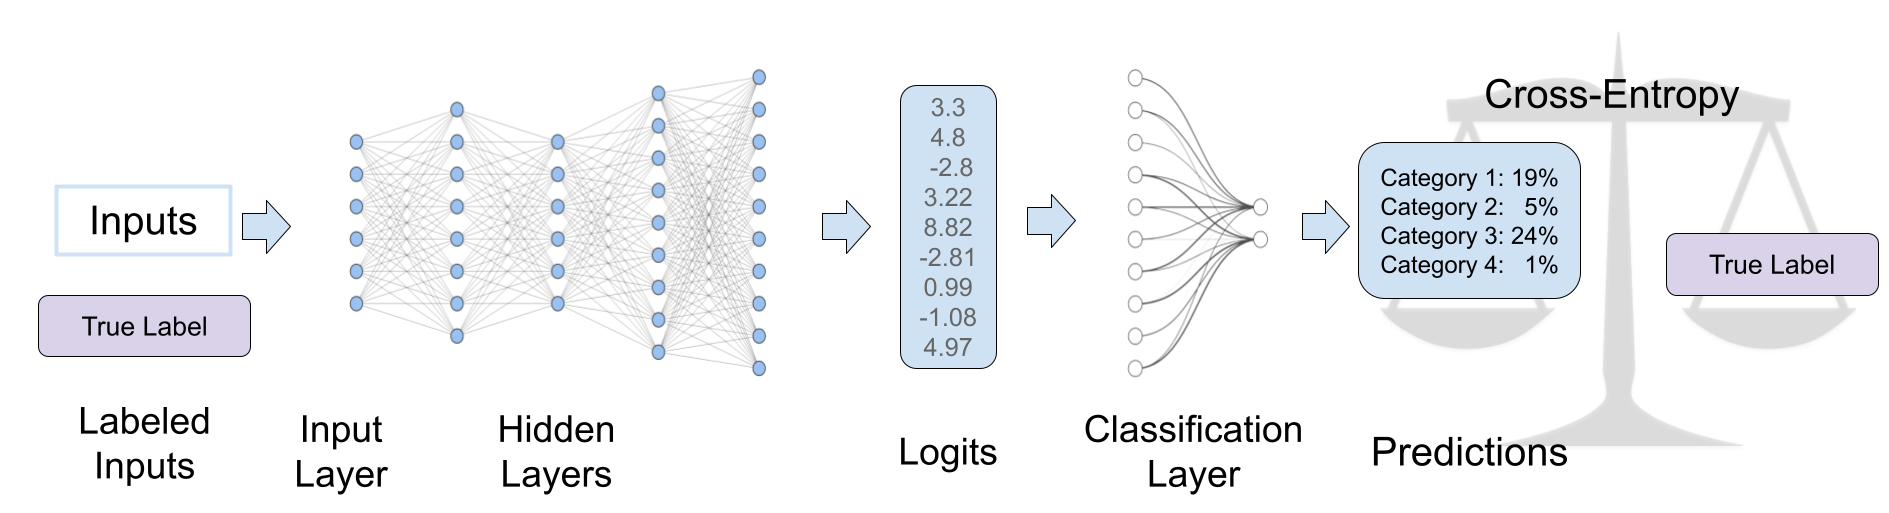
\includegraphics[width=\textwidth]{Figures/02/02_nns_for_classification.png}
    \caption{\neuralNetwork{}s for Classification Tasks}
    \label{fig:02_nn_nns_for_classification}
\end{figure}


% FF NN
% deep vs shallow
% softmax layers
% diagram with the full training cycle

\customHeader{2}{Hyperparameters}
\label{02_nn_hyperparameters}

When training a \neuralNetwork{}, the goal is to fine-tune its parameters or weights to minimize the loss. However, several critical choices need to be made by the designers of the \neuralNetwork{}.

Some decisions concern the \emph{architecture} of the \neuralNetwork{}, such as:

\begin{itemize}
    \item Number of layers
    \item Number of Neurons per layer
    \item Activation functions for each layer
    \item Dimension of output features
    \item Loss function
    \item Optimizer
\end{itemize}

There are also decisions about specific numerical values that affect the training method, such as:


\begin{itemize}
    \item Number of epochs
    \item Learning rate
    \item Batch size
    \item Sizes for the dataset splits
\end{itemize}

All these are known as \emph{hyperparameters}. Unfortunately, there is no one-size-fits-all answer to the question of which hyperparameters to use because the optimal hyperparameters can vary depending on the specific dataset, model architecture, and task at hand. The search space for hyperparameters can be vast, and finding the best combination can be computationally expensive and time-consuming. As a result, the choice of hyperparameters is often determined through trial and error, experimentation, and a combination of domain knowledge and experience.

%% Hyperparameters
% learning rate
% epochs
% batch size
% training, dev, and test split size


%% architecture
% dimension of input features
% activation functions
% number of layers
% neurons per layer

\customHeader{2}{\neuralNetwork{}s for NLP tasks}
\label{02_nn_nlp_tasks}

For \neuralNetwork{}s to handle \gls{nlp} tasks, textual data must be transformed into numerical features to feed to the network. 
A significant advancement in \gls{nlp} came when experts discovered that instead of handcrafting algorithms for feature generation, they could train \neuralNetwork{}s to produce these features for subsequent \neuralNetwork{}s.
The next section elaborates on this approach.



%\clearpage
\customHeader{1}{Tokenization and Embeddings}
\label{02_tokenization_and_embeddings}

Most \gls{nlp} tasks for text start with a corpus of documents. The documents may have been manually collected by humans; automatically collected, for example, using web scrapping tools, generating text from templates, or, most recently, sampling outputs from \gls{ai} tools like GPT-3 \myparencite{wang-etal-2021-want-reduce} and ChatGPT \myparencite{huang2023chatgpt}; or constructed using a mixture of human and automatic input.

Considering the ever-changing nature of natural language, the initial phase in \textclassification{} involves defining the system's Vocabulary. \emph{\tokenization{}} refers to the act of segmenting text into smaller units, known as \emph{tokens}. As a first approach, one may use the intuitive idea of \emph{word} for tokens, in languages with a morphosyntax similar to English (Figure \ref{fig:naive_tokenization}). The collection of unique tokens derived from a text corpus forms the Vocabulary.

\begin{figure}
    \centering
    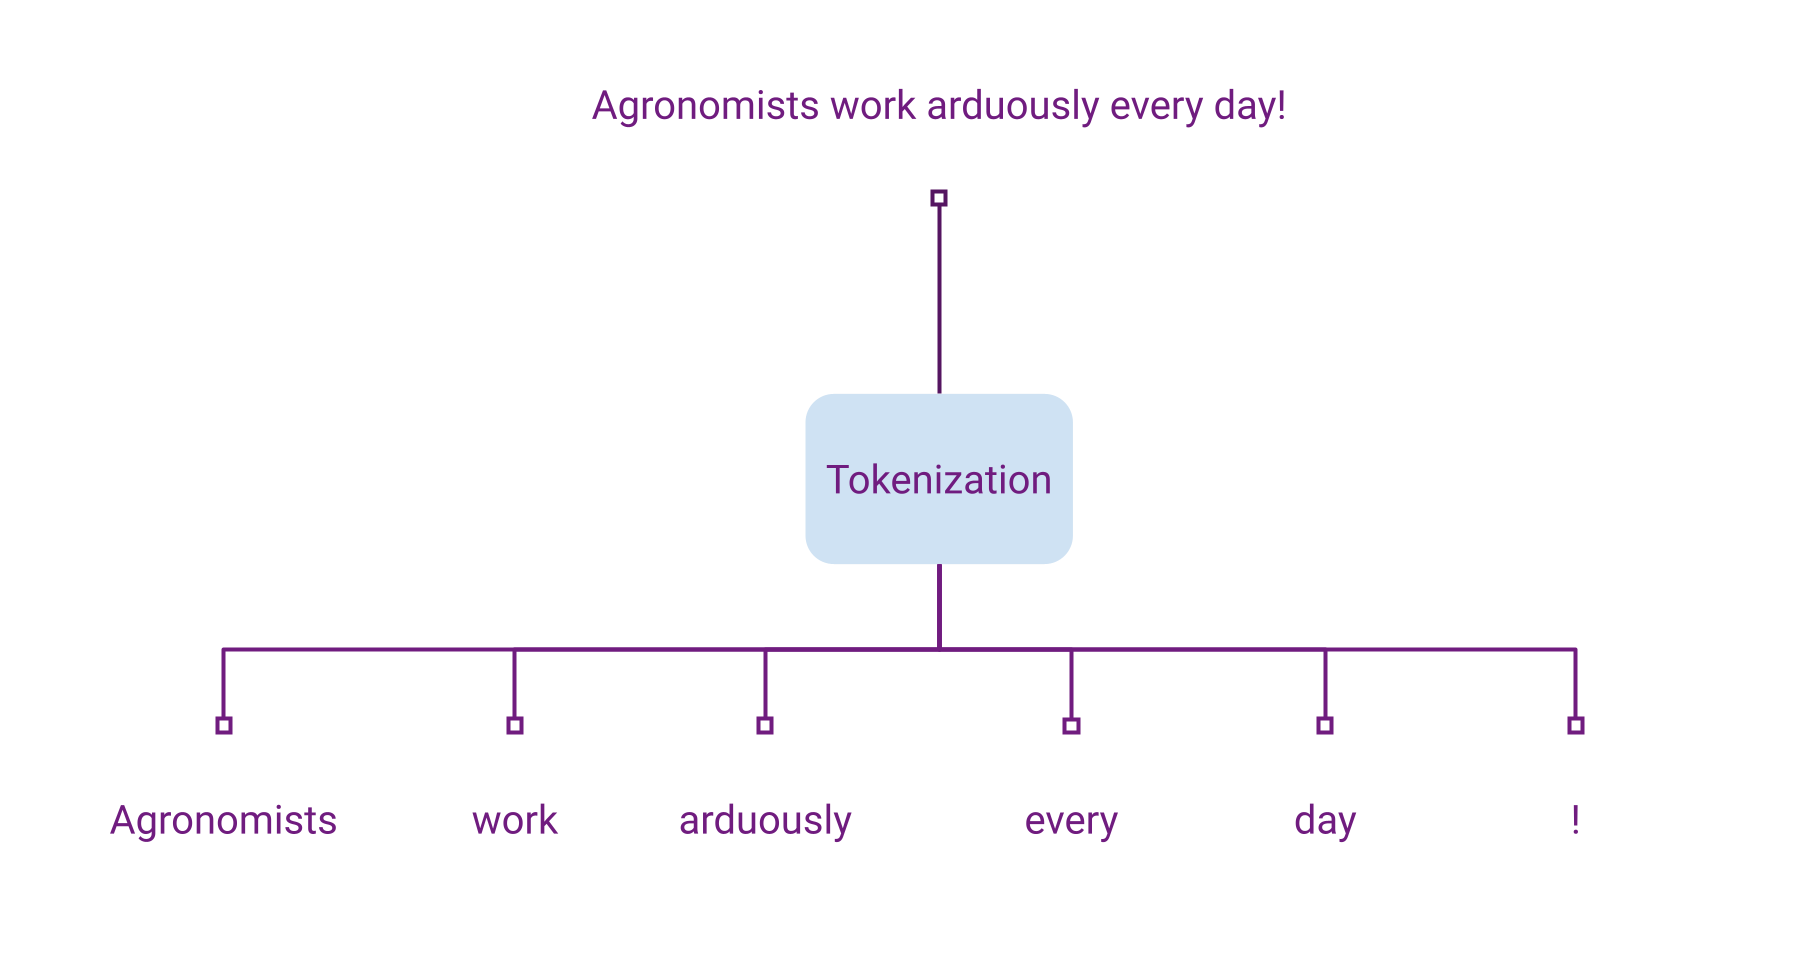
\includegraphics[width=0.75\textwidth]{Figures/02/01_Naive_Tokenization.png}
    \caption{Naive tokenization}
    \label{fig:naive_tokenization}
\end{figure}

However, naive word tokenization\footnote{Another simple tokenization technique is \emph{character-level tokenization}, where text is simply divided into individual characters. This tokenization technique falls outside the scope of this work.} can lead to challenges with out-of-vocabulary (OOV) words when presented with new data. 
A more modern tokenization approach involves using \emph{subword units}. This strategy addresses OOV words by breaking words down into smaller segments. In English, for instance, one might consider prefixes and suffixes as subwords (like \texttt{pre-}, \texttt{-ing}, \texttt{-ed}, and so on), enhancing the \gls{nlp} system's ability to understand morphology. Nevertheless, instead of manually defining rules to divide words into subwords, there are two widely-used algorithms based on character distribution to create such tokenizers:


\begin{itemize}
    \item \emph{\gls{bpe}} \myparencite{sennrich2015neural} builds a vocabulary by iteratively merging the most frequent pair of characters or character sequences in a given text corpus. It starts with a character-level vocabulary and merges the most frequent pair of tokens until a desired vocabulary size is reached.
    \item \emph{\gls{wp}} \myparencite{wu2016google} begins by creating a vocabulary that consists of all the characters found in the training data. It then proceeds to learn a specific number of merge rules. Unlike \gls{bpe}, \wordpiece{} Tokenization selects symbol pairs that maximize their frequency relative to its constituent symbols, rather than choosing the most frequent symbol pair.
\end{itemize}

Typically, these algorithms result in different tokenizations for the same text, leading to different vocabularies. Figure \ref{fig:02_tokenizer_comparison} displays a sample output from the \gls{wp} method in \mytextcite{BERT_paper} and the \gls{bpe} method in \mytextcite{roberta} for English content.


\begin{figure}
    \centering
    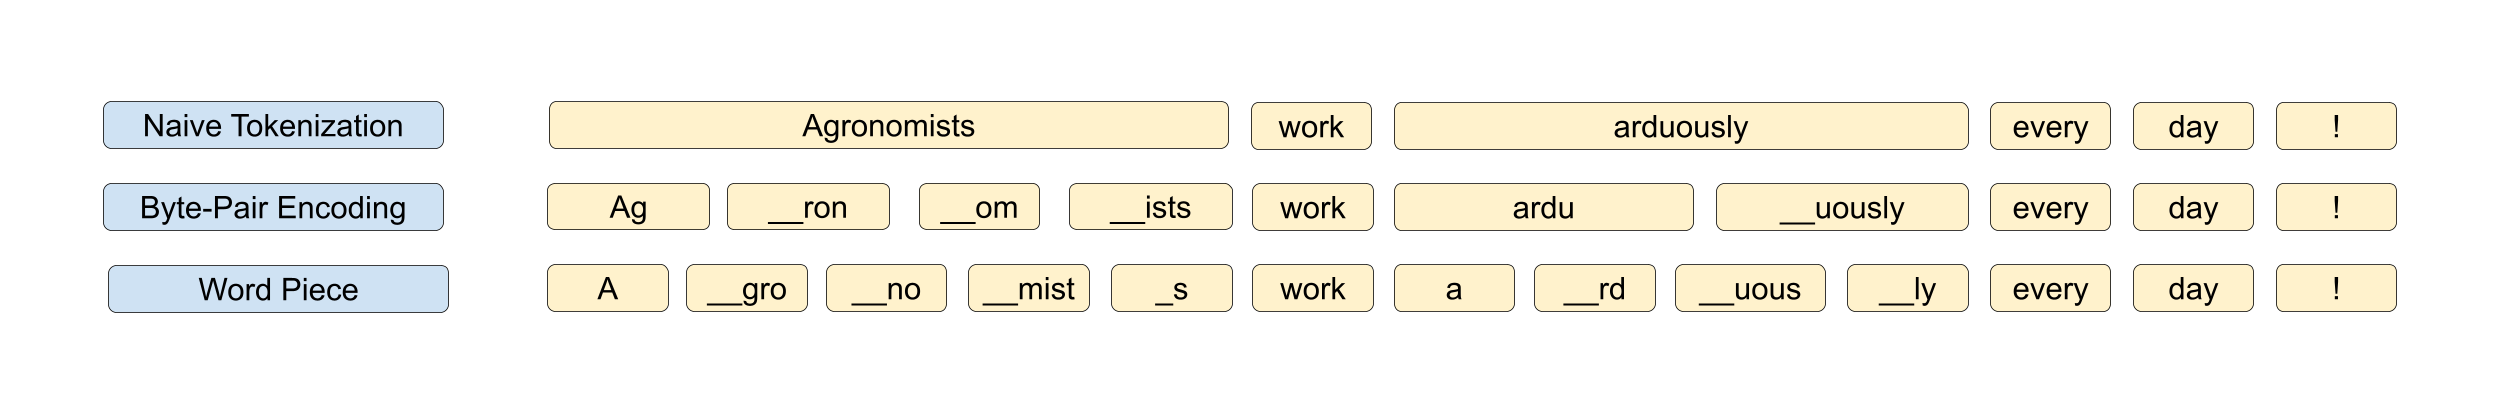
\includegraphics[width=\textwidth]{Figures/02/02_Tokenizer_comparison.png}
    \caption{Different tokenization approaches:\\ naive, \bpe{}, and \wordpiece{}}
    \label{fig:02_tokenizer_comparison}
\end{figure}

Even though there are \textclassification{} approaches which only consider the distribution of tokens in a corpus, like \emph{Naive Bayes Classification} \myparencite{statistical_nlp_naive_bayes}, recent breakthroughs in \gls{nlp} have been enabled by \emph{text embeddings}, which are vector representations of text in high-dimensional space. 

\putInBox{
Embeddings are intended to capture the semantic relationships between texts, allowing computational models to understand and manipulate textual data.  
Typically, embeddings serve as \emph{input features} for textual data, which are then fed into \gls{ml} algorithms (Figure \ref{fig:02_embeddings_for_training_classification}).
}

\emph{Word embeddings} are a type of text embedding that assign a vector representation to each token in a text.
Within \textclassification{}, while word embeddings are prevalent, Document Classification especially benefits from \emph{Document embeddings}. These embeddings provide a unique vector representation for an entire document, enabling a holistic understanding and categorization of texts based on their full content and context. 
Essentially, text embeddings ensure that texts with analogous meanings are closely aligned, while those with divergent meanings are distinctly separated (Figure \ref{fig:word_and_document_embeddings}).


\begin{figure}
    \centering
    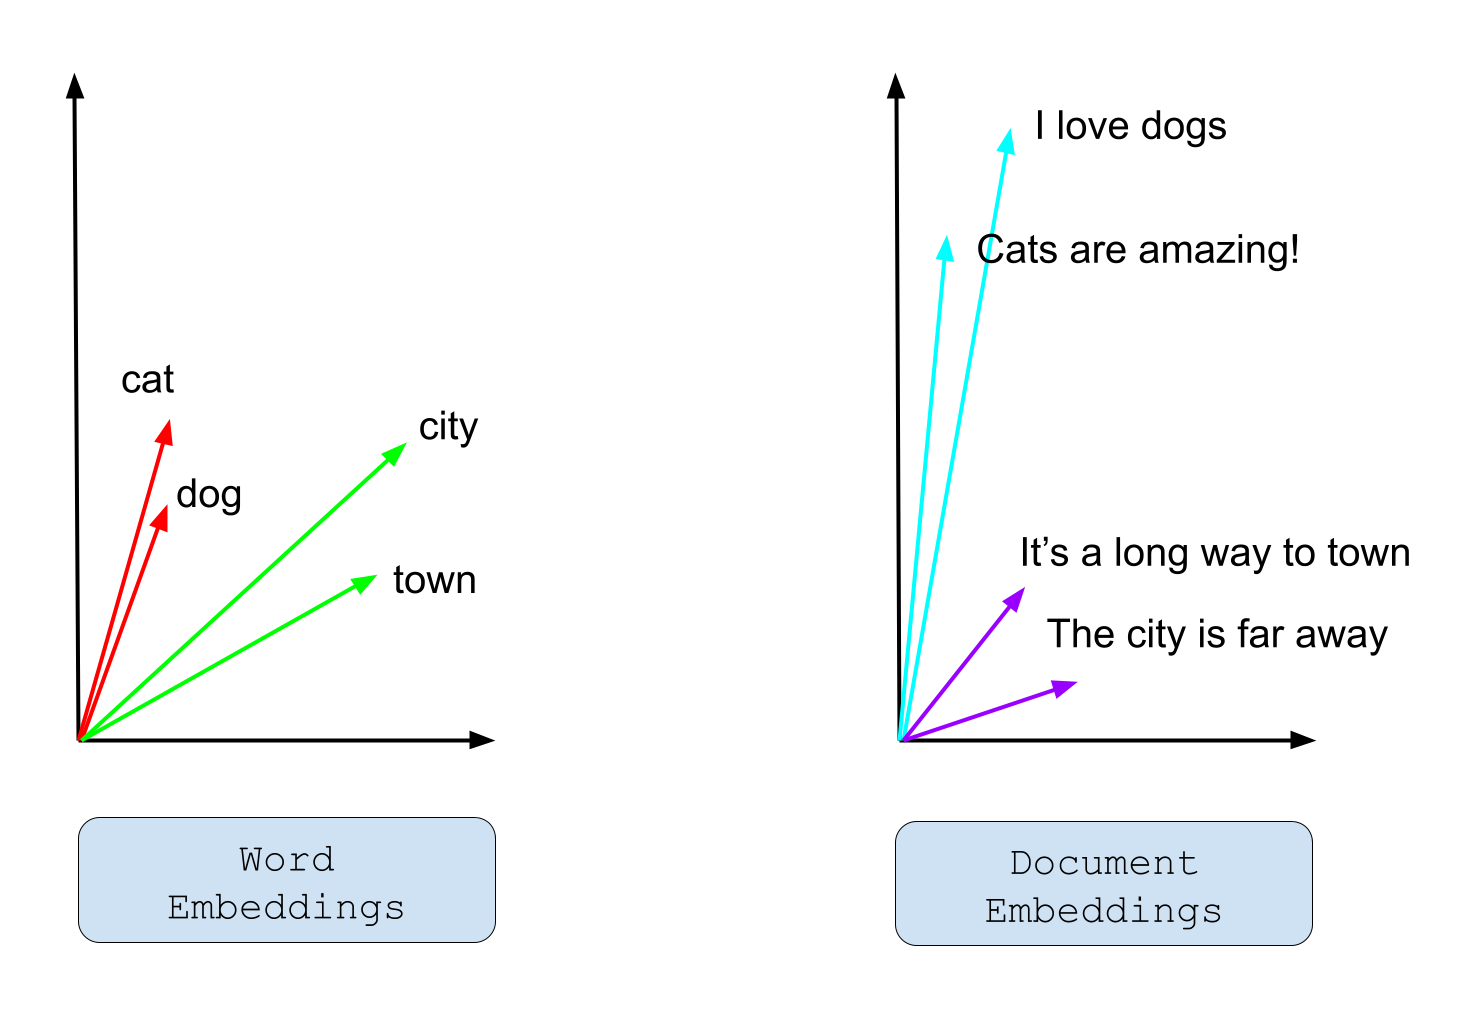
\includegraphics[width=0.5\textwidth]{Figures/02/02_embeddings.png}
    \caption{Word and Document embeddings}
    \label{fig:word_and_document_embeddings}
\end{figure}

\begin{figure}
    \centering
    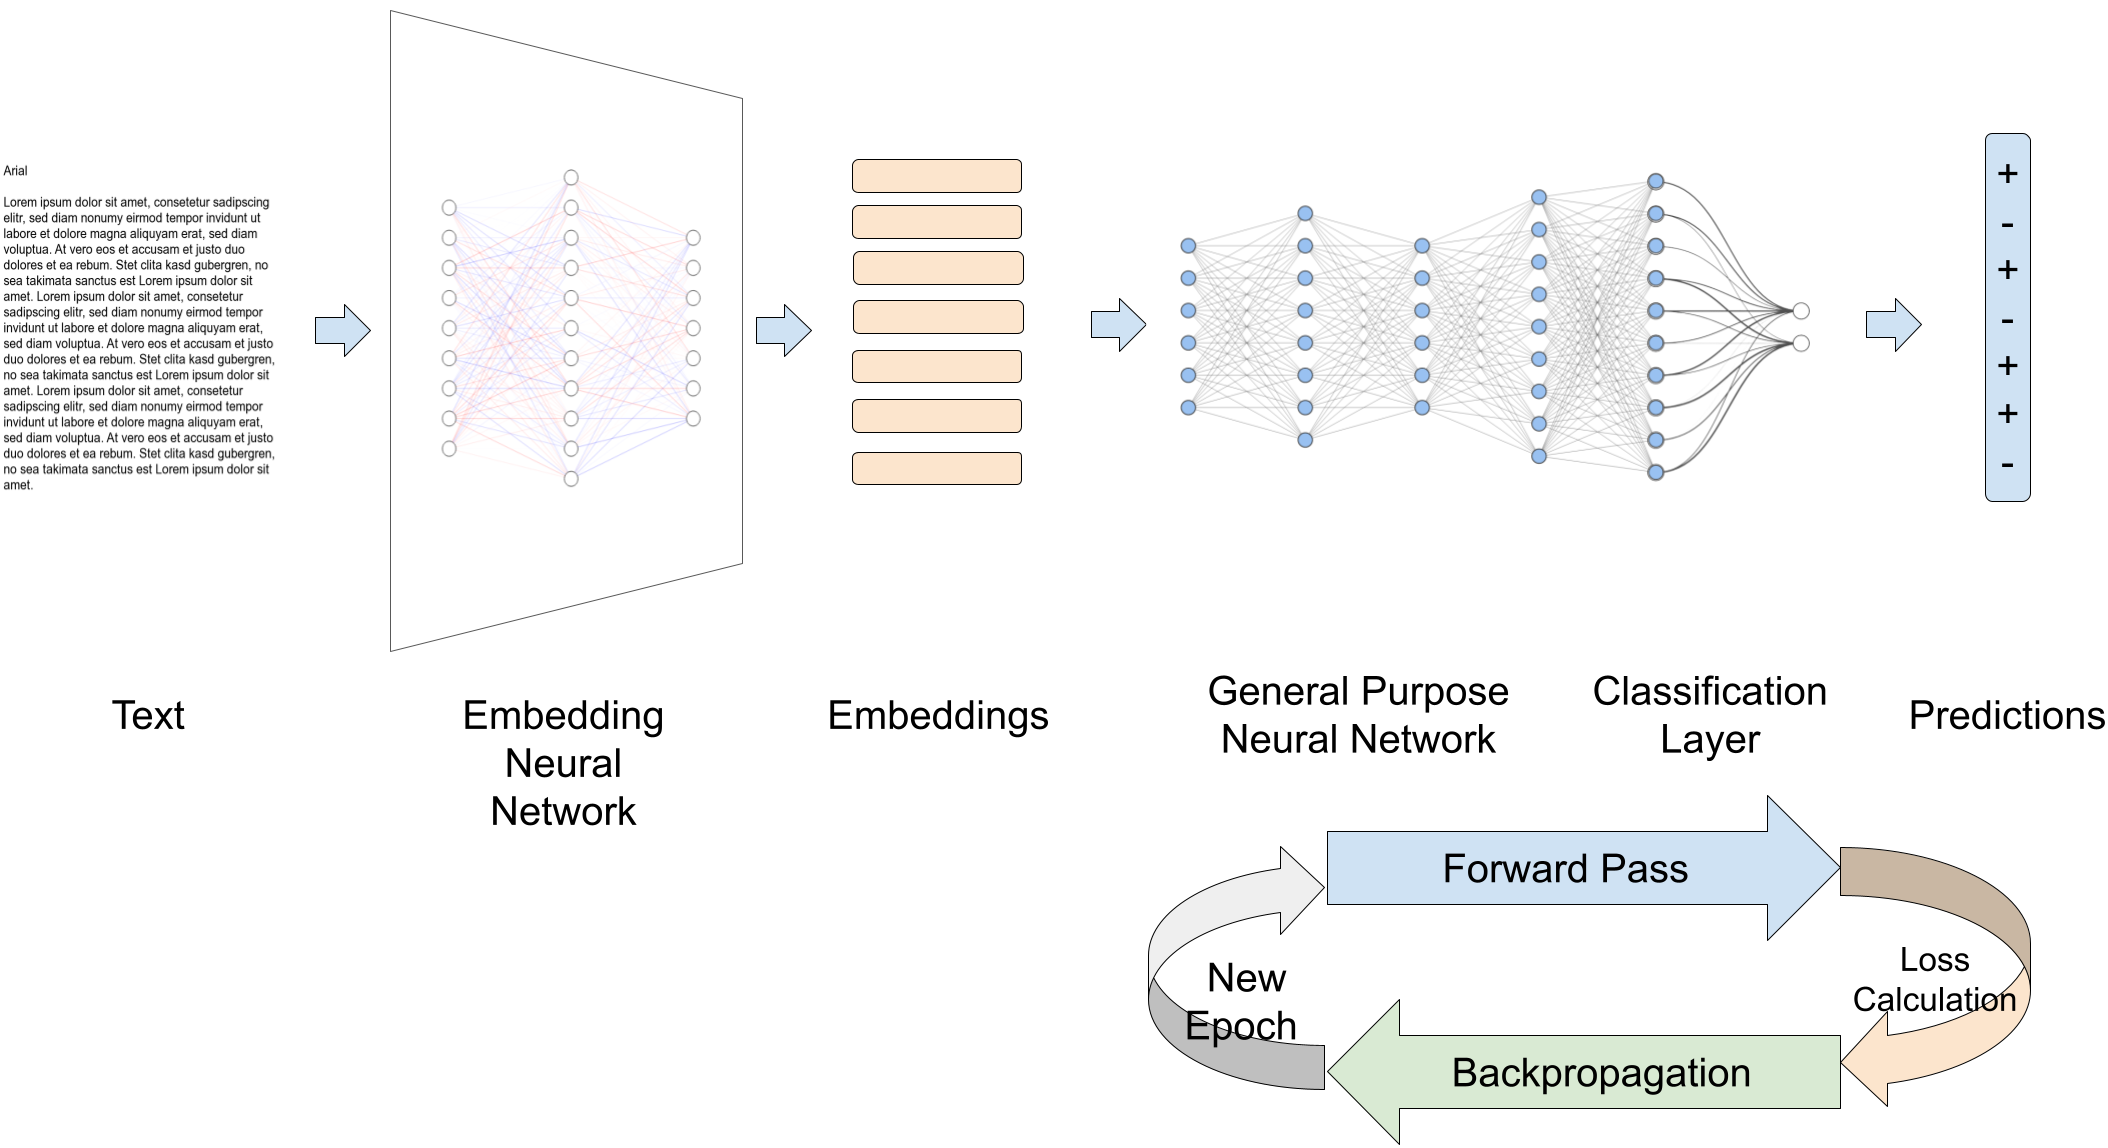
\includegraphics[width=\textwidth]{Figures/02/02_nns_for_nlp.png}
    \caption{Using Embeddings to train Neural Networks for Classification}
    \label{fig:02_embeddings_for_training_classification}
\end{figure}

Text embeddings have undergone significant evolution over the years, with several techniques and models contributing to their development. We present a brief overview of the key milestones in the evolution of word embeddings:

\begin{itemize}
    \item Early approaches focused on frequency-based representations, such as Bag-of-Words (BOW) one-hot encoding\footnote{A one-hot vector has all its components null, except one which has value one} and term frequency-inverse document frequency (TF-IDF). These methods assigned weights or binary values to words based on their occurrence in the corpus, without capturing semantics.
    \item \emph{Word2Vec} \myparencite{mikolov2013linguistic} popularized the concept of word embeddings trained using unsupervised learning. These models utilized shallow neural networks to learn word embeddings by predicting neighboring words or contexts. 
    %\item \emph{GloVe} embeddings \myparencite{pennington-etal-2014-glove}  were trained on word co-occurrence statistics from a large corpus. It leveraged both global word co-occurrence information and local context windows to create meaningful vector representations.
    \item \gls{rnn} architectures, such as GRU (Gated Recurrent Unit), LSTM (Long Short-Term Memory),  and Bi-LSTM (bidirectional LSTM), provided a breakthrough
    by processing sentences sequentially.
    %in capturing sequential dependencies
    %and long-term dependencies 
    %within sentences, 
    For example, with \emph{InferSent} document embeddings \myparencite{infersent_bilstm}. 
    %\gls{rnn}s generated fixed-dimensional vector representations at the sentence level. 
    However, they faced challenges with long-term dependencies and were computationally expensive for longer sentences.
    
    \item  Contextualized word embeddings introduced the idea of generating word representations that varied depending on the context in which the tokens appeared. Models like \emph{ElMo} (Embeddings from Language Models) \myparencite{elmo} and OpenAI's GPT (Generative Pre-trained Transformer) \myparencite{gpt} were able to produce dynamic word embeddings.
    \item Transformer models, including Google's \gls{bert} %(Bidirectional Encoder Representations from Transformers) 
    \myparencite{BERT_paper}, OpenAI's GPT-2 \myparencite{gpt2} and GPT-3 \myparencite{gpt3}, revolutionized the field by leveraging attention mechanisms and large-scale pre-training. These models introduced contextualized word embeddings on a larger scale and achieved state-of-the-art performance across various NLP tasks. %The \BERT{} family of models has gained significant popularity due to its ability to efficiently generate contextualized embeddings for both individual tokens and entire documents at a low cost. Due to this factor, they will serve as primary tools in this project.
\end{itemize}


In this work, our primary focus is on employing the \gls{bert} family of models for \textclassification{}. The details of these models will be explored in the next section.

\customHeader{1}{Evaluation Metrics for Classification}
\label{02_evaluation_metrics}

After obtaining a classifier for Classification tasks, including \textclassification{}, the next step is to evaluate its performance \myparencite{fbetascore}. To achieve this, we use a dataset with known class labels and compare the classifier's \emph{predictions} against these \emph{true} labels. In Binary Classification, there are two classes, and for simplicity we call them the  positive class and negative class; and our primary concern is to measure how the positive class is predicted.

When we apply the classifier to an item, four possible scenarios arise (Table \ref{tab:confusion_matrix}) based on the classifier's predictions and the true class labels.


\begin{minipage}{\textwidth}
\begin{itemize}
    \item True Positives (TP) : The item \emph{is} in the positive class, and the classifier \emph{predicts} the positive class.
    \item True Negatives (TN) : The item \emph{is} in the negative class, and the classifier \emph{predicts} the negative class.
    \item False Negative (FN) : The item \emph{is} in the positive class, and the classifier \emph{predicts} the negative class.
    \item False Positive (FP) : The item \emph{is} in the negative class, and the classifier \emph{predicts} the negative class
\end{itemize}
\end{minipage}

\input{Tables/02/Confusion_matrix}

There are four classic metrics for evaluating classifiers:

\begin{itemize}
    \item Accuracy: Accuracy measures the overall correctness of a classification model. It is the ratio of \emph{correctly} predicted instances to the total number of instances in the dataset.\\
    \begin{align}
    A &= \dfrac{TP + TN}{Positives + Negatives}  \label{eq:def_accuarcy}
\end{align}
    Example: If a model classifies 90 out of 100 samples correctly, the accuracy would be 90\%.
    
    \item Precision: Precision quantifies the ability of a model to correctly identify positive instances among the ones it predicted as positive. It is the ratio of true positive predictions to the total number of positive predictions (both true positives and false positives).
    \begin{align}
    P &= \dfrac{TP}{TP + FP}  \label{eq:def_precision}\\
    \end{align}
    
    Example: If a model predicts 100 instances as positive, and 80 of them are truly positive, the precision would be 80\%. 
    
    Note that, with a model that almost always predicts the negative class, there will be minimal False Positives and True Positives ($FP \to 0$), and thus, this flawed model would have nearly 100\% precision.

    \item Recall (Sensitivity or True Positive Rate): Recall measures the ability of a model to correctly identify all positive instances in the dataset. It is the ratio of true positive predictions to the total number of actual positive instances in the dataset. 

    \begin{align}
    R &= \dfrac{TP}{TP + FN} \label{eq:def_recall}\\
    \end{align}

    Example: If there are 100 positive instances in the dataset, and the model correctly identifies 80 of them, the recall would be 80\%.

    Note that, with a model that almost always predicts the positive class, there will be minimal False Negatives ($FN \to 0$), and thus, this flawed model would have nearly 100\% recall.

    \item \fOne{} Score: The \fOne{} score is the harmonic mean of precision and recall. It balances the trade-off between precision and recall and provides a single metric to evaluate a model's performance.

    \begin{align}
    F_1 &= \left(\dfrac{1}{P} + \dfrac{1}{R}\right)^{-1} \label{eq:def_f1}\\
        &= 2 * \dfrac{P * R}{P + R}
    \end{align}


    Example: If a model has a precision of 75\% and recall of 80\%, the \fOne{} score would be calculated as $2 * ((0.75 * 0.80) / (0.75 + 0.80)) = 77, 4\%$.


    
\end{itemize}

Now that we have discussed the \fOne{} score, let's take a step further and introduce the \fBeta{} score. The \fBeta{} score extends the concept of \fOne{} by introducing a parameter $\beta$, which allows us to control the trade-off between precision and recall. A higher value of beta emphasizes recall, while a lower value emphasizes precision. The \fOne{} score is a special case of the \fBeta{} score when $\beta$ is set to 1.


\begin{align}
    F_\beta &= (1+\beta^2) \dfrac{P * R}{\beta^2* P + R} \label{eq:def_f_beta}
\end{align}


Example: If $\beta$ is set to $2$, the \fTwo{} score will give more two times more weight to recall than precision, making it suitable for tasks where recall is more important than precision, such as ours.

\putInBox{
Our task involves distinguishing between events representing health risks and impacting agriculture (the positive class) from harmless events (the negative class). In this context, it becomes vital to identify as many true positive cases as possible, as they represent actual risks with potential consequences for agriculture. We place a higher priority on this aspect, even if it leads to some harmless events classified incorrectly, because, once our systems predict a positive event, subject experts will be alerted and will proceed to take a final decision.
Consequently, our priority lies in emphasizing recall over precision. Hence, we opt to evaluate our systems using the \fTwo{} score.


\todo{Check the style of this paragraph.}
}



\customHeader{2}{Evaluating Probabilistic Classifiers}
\label{02_evaluating_probabilistic_classifiers}

A probabilistic binary classifier is a type of classifier that provides the probability of an item belonging to the positive class rather than making a definitive decision. To ultimately classify items, a threshold or cut-off point is required. For instance, a threshold of 50\% may be set, considering items with probabilities above this threshold as positive and those below as negative. Additionally, this threshold can be adjusted to be more stringent, requiring a higher confidence level (e.g., 60\%) for positive classification, or more lenient, allowing lower confidence (e.g., 40\%) for positive classification, and so on \myparencite{auc_definition}.

When evaluating a probabilistic classifier with a labelled dataset, varying thresholds result in different confusion matrices. Leveraging this observation, we can establish a metric to assess probabilistic classifiers. To begin, we must introduce two key concepts.

\begin{itemize}
    \item The True Positive Rate (TPR)  is calculated as the proportion of True Positive predictions to all actual Positive instances, that is, it is simply the recall (Equation \ref{eq:def_recall}). It measures the classifier's performance with respect to the positive portion of the dataset.

    \begin{align}
        TPR &= \dfrac{TP}{TP+FN} =R \label{def_tpr} 
    \end{align}
    
    \item The False Positive Rate (FPR) is calculated as the proportion of False Positive predictions to all actual Negative instances. It measures the classifier's performance with respect to the negative portion of the dataset, in an inverse way \footnote{That is, higher FPR means worse performance regarding the negatives, and lower FPR means better performance.} (See equation \ref{def_fpr_2}).
    
    \begin{align}
        FPR &= \dfrac{FP}{TN+FP} \label{def_fpr} \\
            &= 1 - \dfrac{TN}{TN+FP} \label{def_fpr_2}
    \end{align}
    
\end{itemize}

The crucial observation is that selecting a fixed probability threshold yields specific values in the confusion matrix, thereby determining a corresponding pair of values $(FPR, TPR)$. These values can be plotted on a plane, resulting in a curve known as the \emph{Receiver Operating Characteristic} (ROC) curve, as the threshold varies.

To introduce the \gls{auc} measure, we first need to make some observations  about the ROC curve (Figure \ref{fig:02_auc}):

\begin{enumerate}
    \item A threshold of 0\% implies that every item is classified as a positive, thus, there are no True Negatives and no False Negatives, which means that the FPR and TPR are both 1.

    \item A threshold of 100\% implies that every item is classified as a negative, thus, there are no True Positives and no False Positives, which means that the FRP and TPR are both 0.

    \item Combining these two observations, if we plot the curve by decreasing the threshold from 100\% to 0\%, we will obtain a curve starting from point $(0,0)$ and ending at point $(1,1)$.

    \item A perfect classification system would make no mistakes, no matter the probability threshold\footnote{Except for thresholds of 0\% and 100\%, as explained above}. That is, it would have no False Positives and no False Negatives. This would make the TPR always 1, which corresponds to a horizontal line 1 unit above the horizontal axis. 

    \item A completely inaccurate classification system is always wrong, no matter the probability threshold. That is, it would never have True Positives nor True Negatives. This would make the TPR always 0, which corresponds to a horizontal line on top of the horizontal axis.

    \item A classification system that always takes decisions at random, is equally likely to correctly identify positive instances as it is to incorrectly label negative instances as positive. This means, the FPR and TPR would always be equal, which corresponds to a diagonal line.

    \item A classification system that performs better than a random classifier will have a performance tending towards a perfect classifier, which corresponds to a curve above the diagonal.

    \item A classification system that performs worse than a random classifier will have a performance tending towards a completely inaccurate classifier, which corresponds to a curve below the diagonal.

\end{enumerate}

\begin{figure}
    \centering
    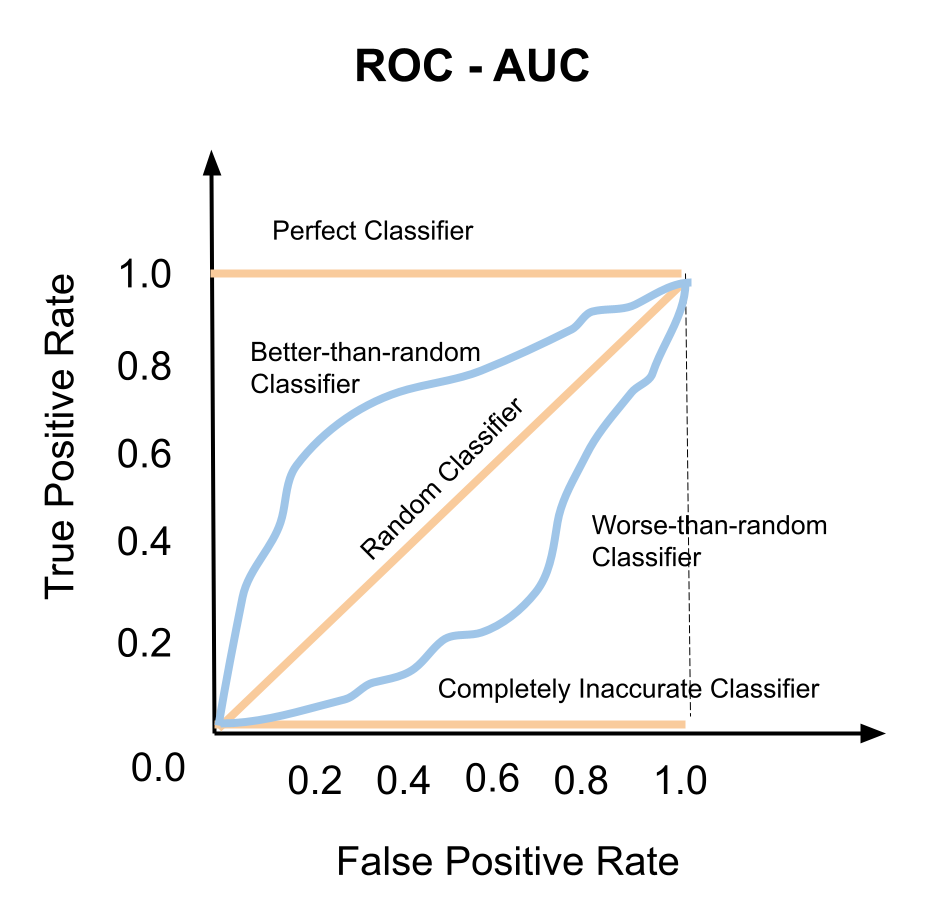
\includegraphics[width=0.5\textwidth]{Figures/02/02_AUC.png}
    \caption{Area Under Curve}
    \label{fig:02_auc}
\end{figure}


Thus, we may use the area under the ROC curve to evaluate probabilistic classifiers:

\begin{itemize}
    \item A perfect classifier has an \gls{auc} of 1.0
    \item A completely inaccurate classifier has an \gls{auc} of 0.0
    \item A random classifier has an \gls{auc} of 0.5
    \item A better-than-random classifier has an \gls{auc} above 0.5
    \item A worse-than-random classifier has an \gls{auc} below 0.5
\end{itemize}


\customHeader{1}{\BERT{} Models for \textclassification}
\label{02_bert_models_for_text_classification}

A \emph{Language Model} is a \neuralNetwork{} that can be used for predicting the distribution of tokens, given a corpus. The main goal of a Language Model is to capture the underlying patterns and structure of tokens in the corpus.
The architecture for the \gls{bert} (Bidirectional Encoder Representations from Transformers) family of models was introduced \mytextcite{BERT_paper} as one capable of learning embeddings aware of the left and right context for each token\footnote{Hence the name ``Bidirectional".}. 
\putInBox{
The \BERT{} family of models has gained significant popularity due to its ability to efficiently generate contextualized embeddings for both individual tokens and entire documents at a low cost \myparencite{revolution_bert}.
}
While the original \gls{bert} is a general-purpose model, many tasks benefit from domain-specific knowledge. The multitude of \gls{bert} models arises from the need to cater to different languages, domains, tasks, and computational constraints, combined with ongoing research efforts to improve model performance and efficiency. 

Many \gls{bert} models are freely and readily accessible and set for deployment across a range of \gls{nlp} tasks. Given this availability, they will serve as primary tools for this work.



\customHeader{2}{Attention and Transformers}
\label{02_attention_and_transformers}


For many years, \gls{nlp} methods faced challenges with understanding distant relationships within texts. For example, consider the sentence, ``The cat, which was adopted from the shelter last month, loves to play.". Here, the subject (cat) and the verb (loves) are spaced apart by several words, making it tricky for systems identifying grammatical roles. Similarly, when translating from, say, Japanese to English, it's crucial to recognize that the Japanese verb typically appears at the end of the sentence. 

Initially introduced in \gls{nlp} for Machine Translation \myparencite{attention_for_translation}, the \emph{Attention} mechanism enables the \neuralNetwork{} to focus on particular words or phrases crucial for grasping the context. 
It achieves this by employing trainable parameters to determine coefficients between 0 and 1, indicating the significance of each input token to each output token (Figure \ref{fig:02_attention_for_translation}). The part of the network responsible for determining these attention coefficients is termed an \emph{Attention Head}.

Interestingly, attention can be computed between a sentence and itself to evaluate the significance of its various components relative to one another; this process is called \emph{Self-Attention}. The outcome of the Self-Attention mechanism for a text comprising $n$ tokens is an $n\times n$ matrix $A=(a_{ij})$, where $a_ij$ is a value between 0 and 1, denoting the influence of token $j$ on token $i$ (typically, $p_{ij}\neq p_{ji}$). In the original architecture, which we employ in this work, the time and memory usage for Self-Attention grow in a quadratic manner on the text's length ($O(n^2)$). More recent Self-Attention designs aim to reduce computing time \cite{flash_attention}.


\begin{figure}
    \centering
    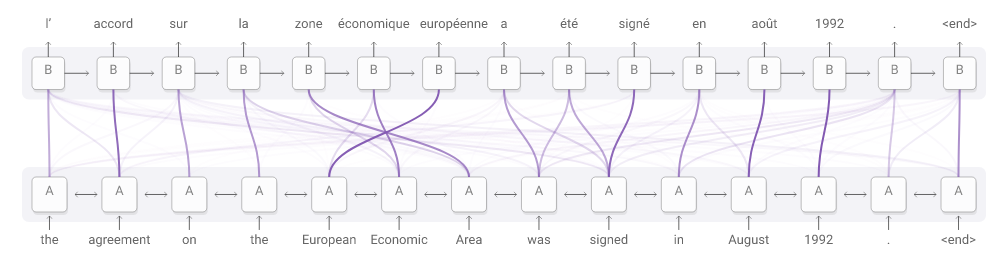
\includegraphics[width=.75\textwidth]{Figures/02/Attention_for_translation.png}
    \caption{Attention Mechanism for Machine Translation, from \mytextcite{attention_distilled}}
    \label{fig:02_attention_for_translation}
\end{figure}


Attention mechanisms are a fundamental component of \emph{Transformer} models, a type of deep learning architecture that has revolutionized \gls{nlp} tasks. The original Transformer model, introduced in the ``Attention is All You Need" paper by \cite{attention_is_all_you_need}, uses multiple a Self-Attention Heads, and is primarily used for sequence-to-sequence tasks, such as Machine Translation.

A classical Transformer architecture consists of two main neural modules, the \emph{Encoder} and the \emph{Decoder}. The encoder module takes embeddings as input features, computes self-attention, and produces attention-enriched embeddings.
These enhanced embeddings are then channeled to the decoder, which outputs the logits of the probabilities of the next token.
Notably, the decoder also incorporates its prior outputs as inputs, applies self-attention to them, and then calculates "cross" attention between these and the attention-augmented embeddings from the encoder. The design of this architecture is depicted in Figure \ref{fig:02_transformer_architecture}.

After successful training, the encoder learns the optimal way to generate embeddings for each token considering all the other tokens in the input. At the same time, the decoder learns to produce tokens in a manner informed by the input and its own output. Due to the quadratic complexity of Self-Attention, Transformer architectures have a limited input size.


\begin{figure}
    \centering
    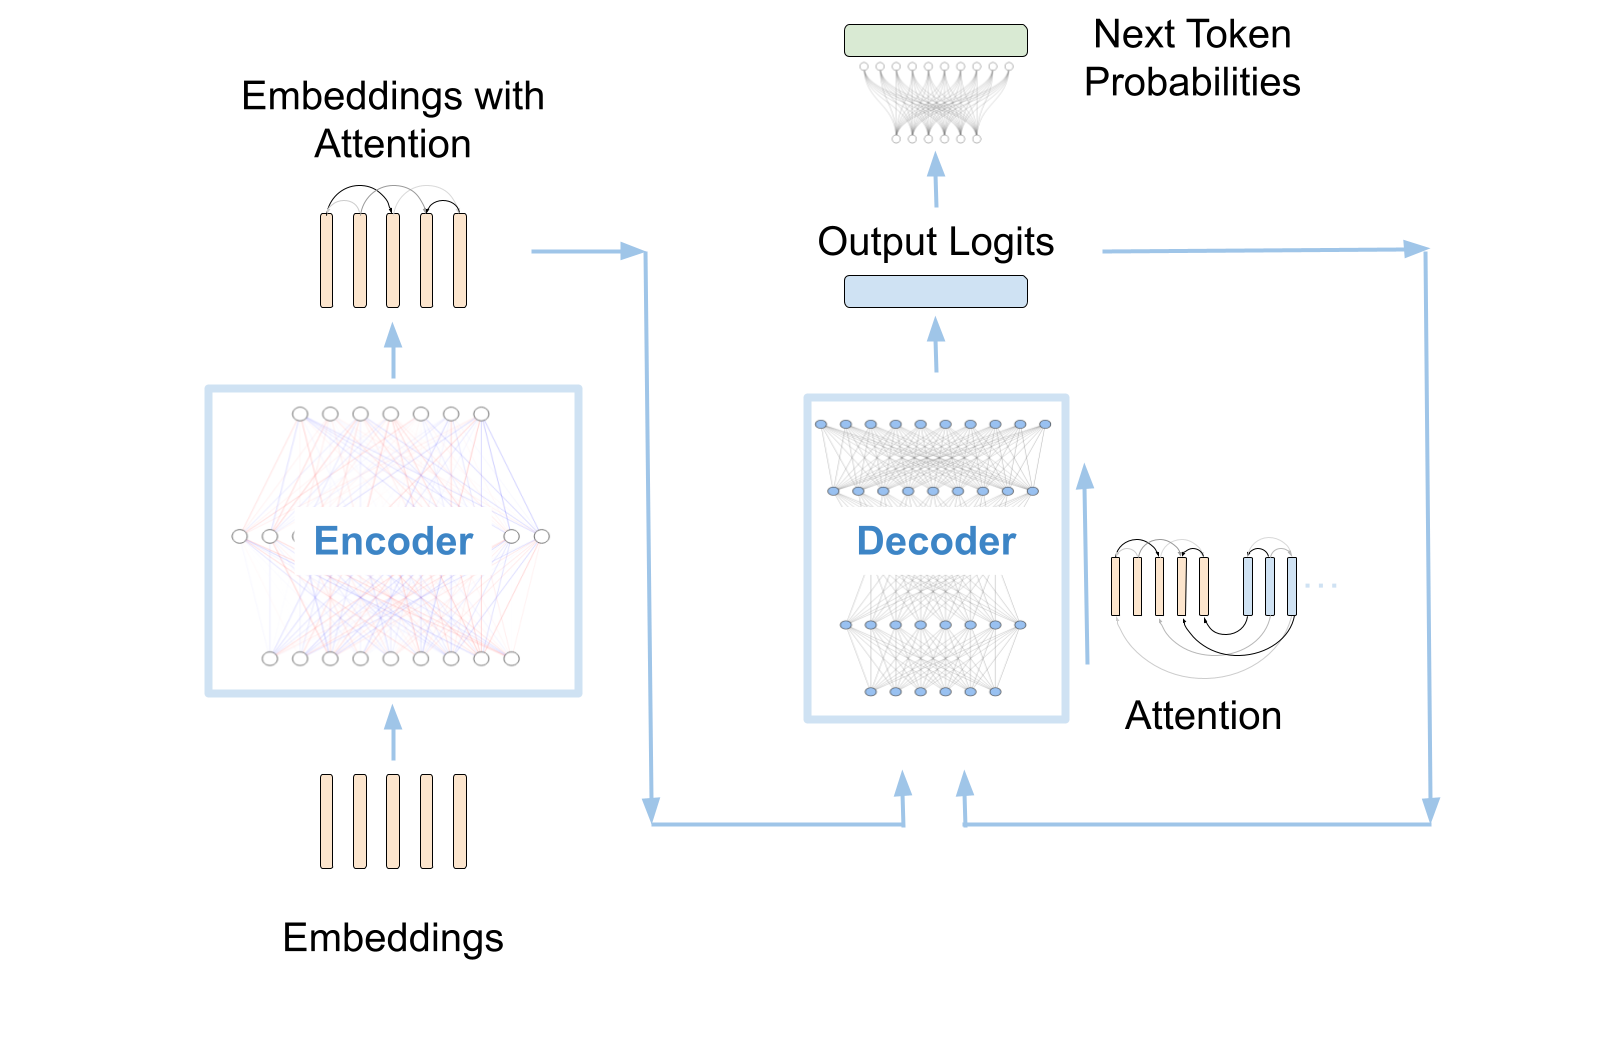
\includegraphics[width=0.75\textwidth]{Figures/02/02_transformer.png}
    \caption{Classical Transformer Architecture}
    \label{fig:02_transformer_architecture}
\end{figure}







\customHeader{2}{The training of \BERT{}}
\label{02_training_bert}

The architecture for \gls{bert}  essentially a series of encoder modules from the traditional Transformer design, layered sequentially\footnote{Hence the name ``Encoder Representations from Transformers".}. 
Two distinct versions were introduced by the original auhors for English text: a base model with 12 encoder layers and 12 attention heads, yielding 768-dimensional embeddings, and a large model with 24 encoder layers and 16 attention heads, resulting in 1024-dimensional embeddings. The basic \gls{bert} architecture employs a \gls{wp} tokenizer and can handle up to 512 tokens as input.

For training \gls{bert} to generate context-aware embeddings for individual tokens as well as entire sentences, it was subjected to two specific tasks. The datasets utilized for this purpose were Google's BookCorpus and the English portion of Wikipedia.

\customHeader{3}{Masked Language Modeling}
\label{02_mlm}

To learn embeddings for tokens, the authors introduce the \gls{mlm} task.
At its core, the \gls{mlm} task aims for the model to ``fill-in the blank" or to ``guess the missing word". For \gls{mlm}, once a text is tokenized, 15\% of the tokens are randomly substituted with a unique \texttt{[MASK]} token, symbolizing a blank space. This modified sequence is then processed by the encoder layers, relying on the self-attention mechanisms to provide sufficient contextual understanding (as depicted in Figure \ref{fig:02_attention_mlm}). To determine the omitted word, the final embedding corresponding to the \texttt{[MASK]} token is passed through a \gls{softmax} activation function, yielding a probability distribution over all the tokens in the vocabulary. By contrasting these probabilities with the known token, the cross-entropy loss is computed, which serves as the loss to be minimized. This procedure enables \gls{bert} to learn about the token distribution.



\begin{figure}
    \centering
    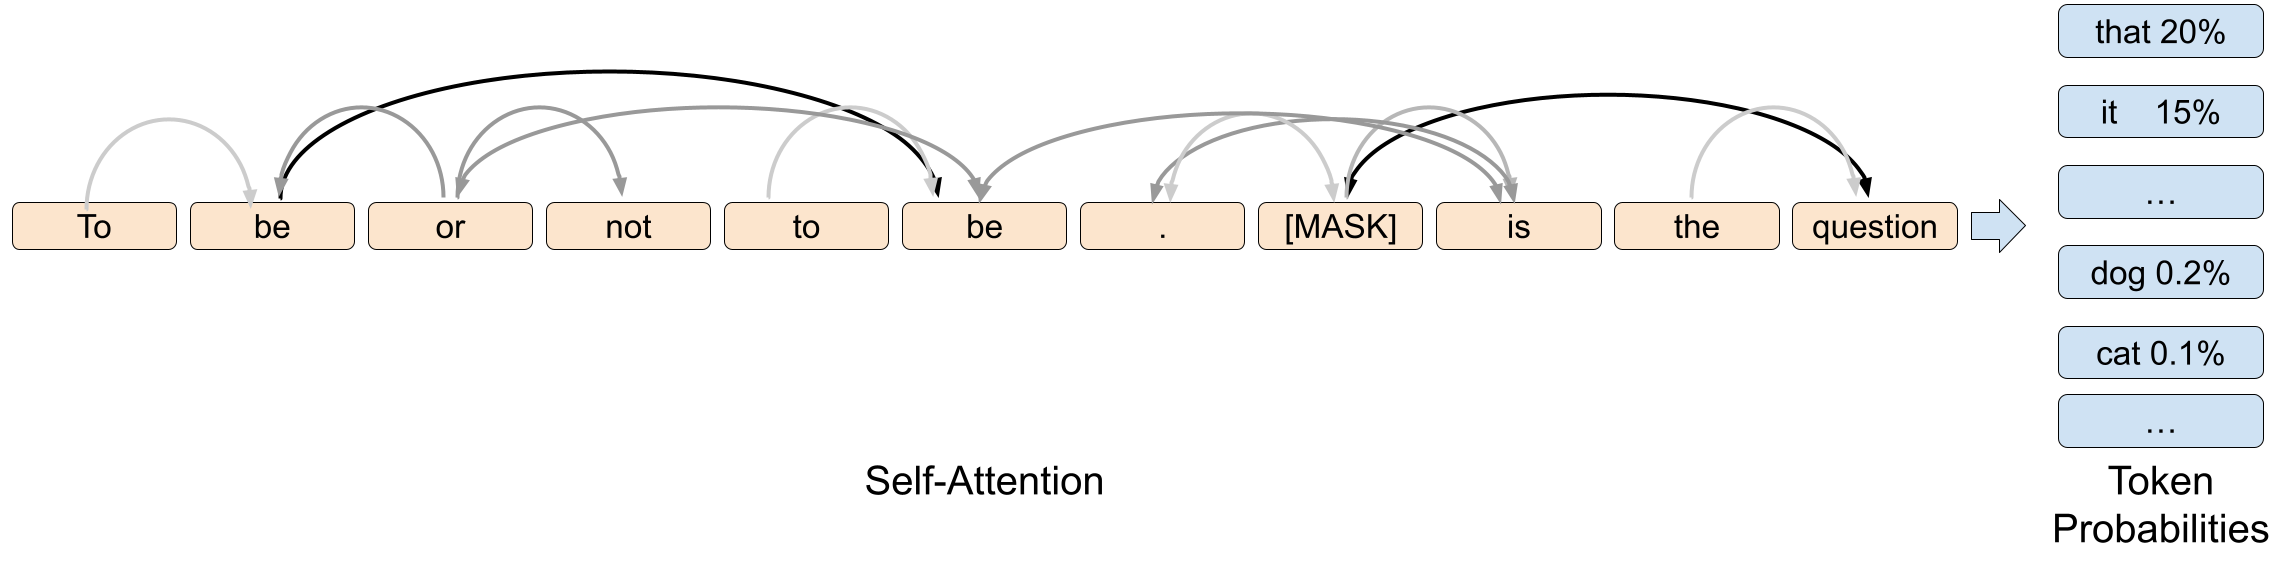
\includegraphics[width=\textwidth]{Figures/02/02_mlm.png}
    \caption{Self-Attention for MLM}
    \label{fig:02_attention_mlm}
\end{figure}

\customHeader{3}{Next Sentence Prediction}
\label{02_next_sentence_prediction}


To learn embeddings for sentences, the Next Sentence Prediction task used by the authors involves joining two sentences or phrases and training the model to determine if they appeared consecutively in the training dataset. 
Specifically, for each example with sentences $A$ and $B$, there's a 50\% chance that $B$ is the actual subsequent sentence to $A$, and a 50\% chance it's a random sentence from the dataset. 
In order to do this, the authors introduce two special tokens, the \texttt{[CLS]} token, for classification, and the \texttt{[SEP]} token to  separate the texts. 

During training, the \texttt{[CLS]} token is placed at the start of the text, and the \texttt{[SEP]} token is positioned between the two sentences. After processing by the encoders, the \texttt{[CLS]} token's embedding undergoes further refinement via a \emph{Pooling Layer}\footnote{This layer comprises a linear layer with a \gls{tanh} activation function}, resulting in what's termed the aggregated or \emph{pooled} output. This pooled output aims to encapsulate the entire text's meaning. Ultimately, this output is fed into a classification layer, and the generated probabilities are matched against the known sentence distribution to compute the cross-entropy (as illustrated in Figure \ref{02_next_sentence_prediction}). Through this process, \gls{bert} is trained to generate embeddings that represent whole sentences.



\begin{figure}
  \makebox[\textwidth][c]{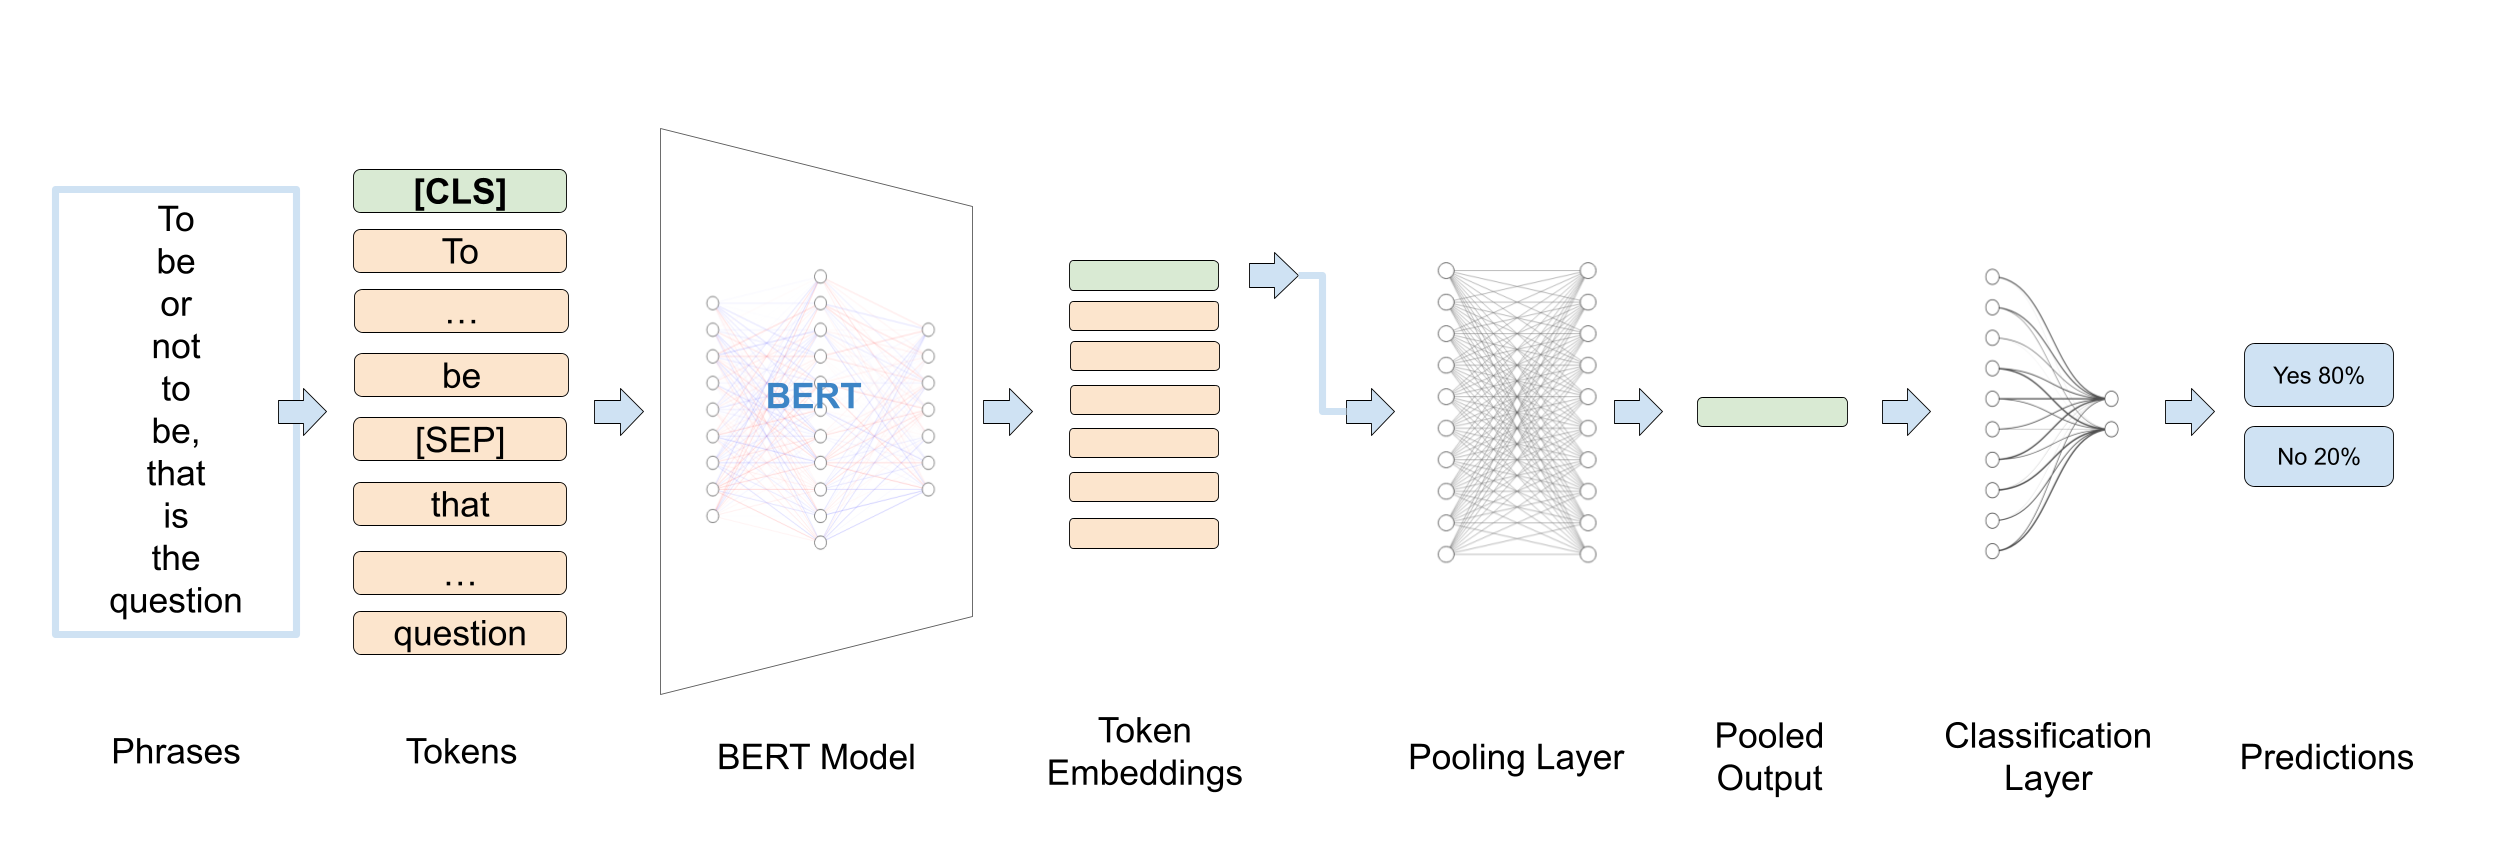
\includegraphics[width=0.9\paperwidth]{Figures/02/02_next_sentence_prediction.png}}%
  \caption{Next Sentence Prediction Task for \BERT{}}
  \label{fig:02_next_sentence_prediction}
\end{figure}



\customHeader{2}{Using \BERT{} for \textclassification{}}
\label{02_using_bert_for_text_classification}


The training process for \gls{bert} doesn't require the texts to be labeled or categorized, making it an \emph{unsupervised} approach. This approach allowed \gls{bert} to learn general text representations that encompass a variety of syntactic and semantic patterns across diverse contexts.

\putInBox{
Once the \gls{bert} model is trained, the conventional method for Document Classification using \gls{bert} involves feeding the text to the model\footnote{keeping the second sentence empty after the \texttt{[SEP]} token}. Then, the pooled output serves as the document's embedding. This embedding is then fed to a classification layer, which is further trained for the specific task at hand (as illustrated in Figure \ref{fig:02_bert_for_document_classification}).
}


\begin{figure}
    \centering
    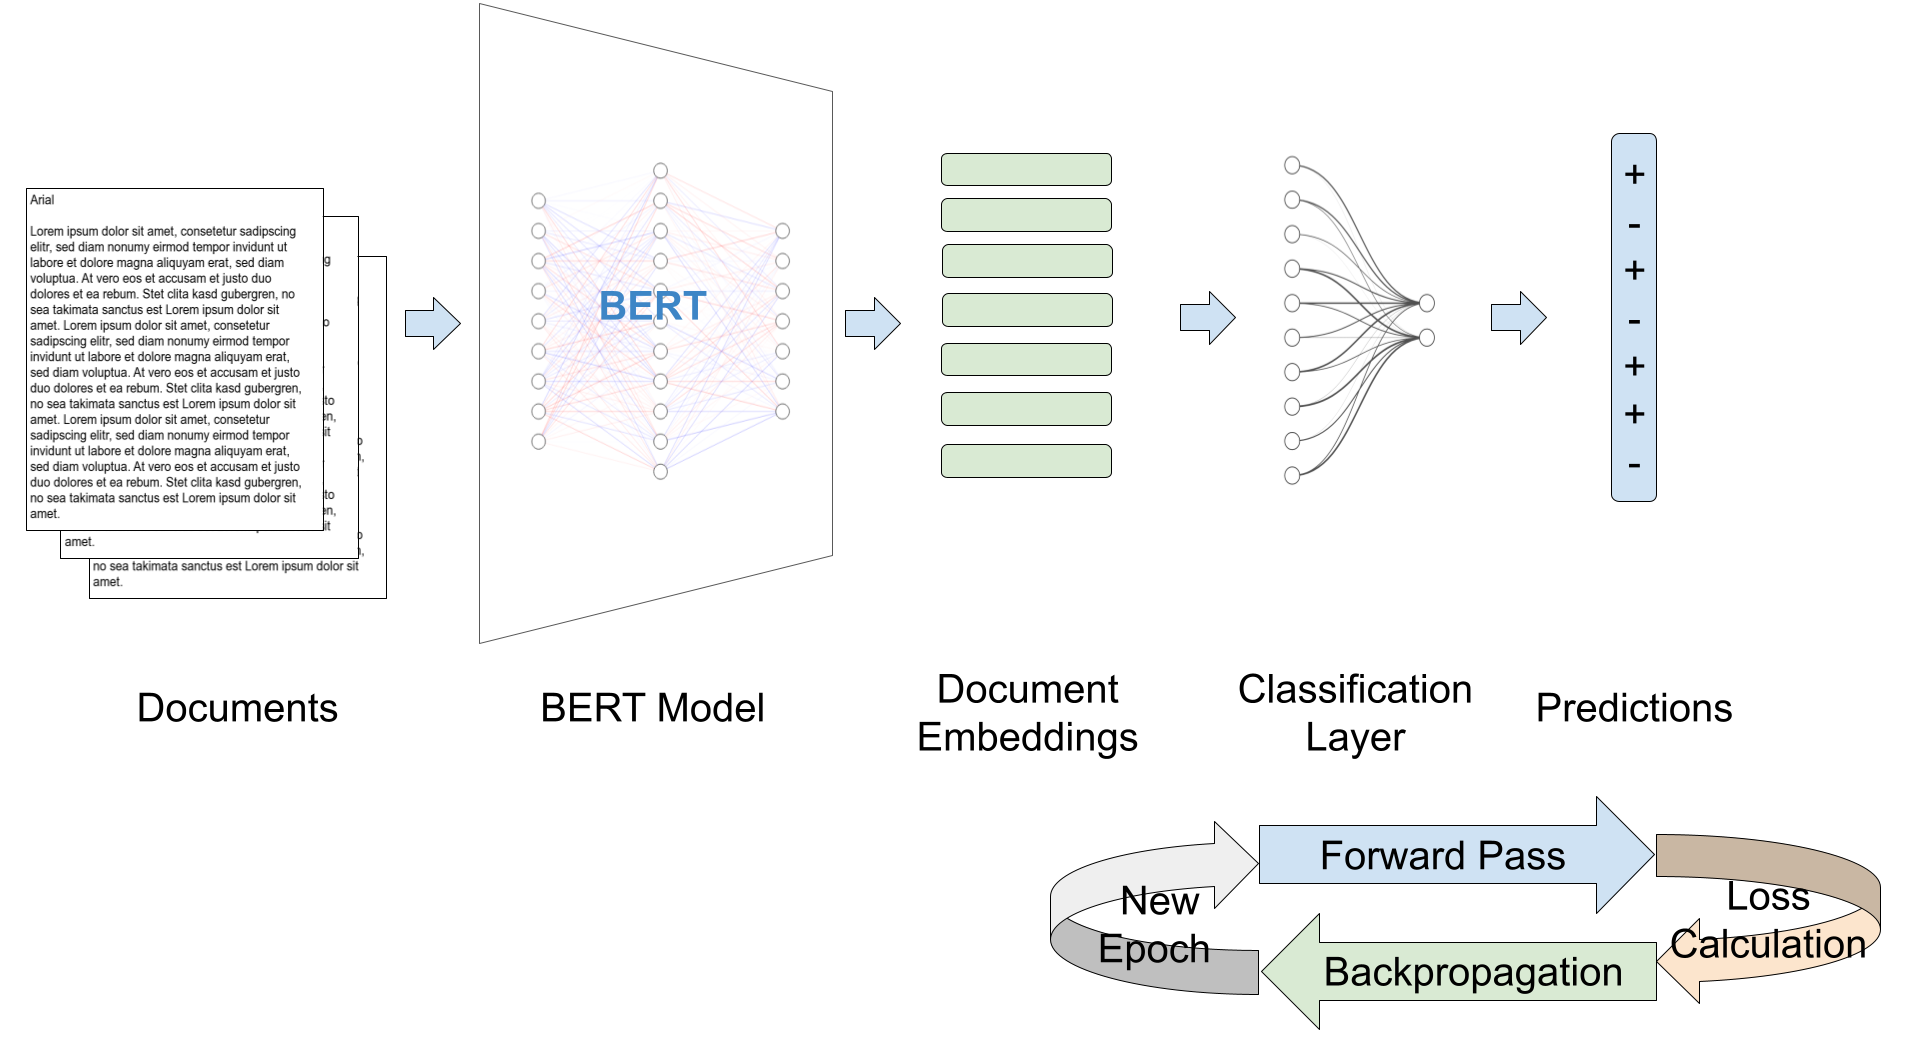
\includegraphics[width=\textwidth]{Figures/02/02_BERT_for_document_classification.png}
    \caption{Using \BERT{} Embeddings for Document Classification}
    \label{fig:02_bert_for_document_classification}
\end{figure}




% Self Attention
% Training
% MLM, next sentence prediction

% input size, attention heads, layers, 
% CLS, pooled output




\customHeader{1}{Feature based \textclassification{}}
\label{02_feature_based_text_classification}

For this project, we focus on \textclassification{} methods based on textual features, which are ways of representing the meaning of a piece of text as a vector, that is, as an ordered array of numbers.
\todo{Complete this}



\newpage
\customHeader{0}{Related Work}
\label{03_related_work}


As in almost all industries, \neuralNetwork{}s-based \gls{ai} is being adopted in Agriculture \myparencite{ai_for_agriculture}. Some of the most prominent uses of \gls{ai} and Deep Learning have been the automatization of decisions or alerts produced by sensors \myparencite{sensors_for_agriculture};  and the use of the \href{https://en.wikipedia.org/wiki/Internet_of_things}{Internet of Things}\footnote{\url{https://en.wikipedia.org/wiki/Internet_of_things}} to integrate sensors and software, in order to warn farmers of possible issues with their crops \myparencite{iot_for_agriculture}. 

On the other hand, the application of \gls{nlp} to Agriculture, and especially to Epidemiological Surveillance, has been rather timid. A popular approach has been to use data mining from social media to gather textual data \myparencite{data_mining_for_plant_health}. Twitter has been used as a source of crowdsourced knowledge about ecological events \myparencite{twitter_detect_influenza_epidemics_2011, social_media_disease_surveillance_2015_no_bert}. However, there have been concerns about the reliability of social media data for Epidemiological Surveillance, as the public and the agricultural workers may lack the specialized knowledge to accurately assess risks \myparencite{limitations_of_social_media_for_biosecurity_events}.


Moreover, until recently, the advancements in Neural Network-based Language Models didn't significantly influence \gls{nlp} applications in Epidemiological Surveillance \myparencite{BioMedicalBERT_ALBERT_ELECTRA_2021, BioNER_with_multilingualBERT_2019}.
This landscape shifted during the COVID-19 Pandemic when both computer vision and \gls{nlp} emerged as vital tools for diagnosis, prevention, and notably for our work, monitoring the spread of the disease. Still, these technological strides haven't been extensively applied in the field of Plant Health Surveillance.


\mytextcite{social_media_crop_health_monitoring} introduced the idea of using social media data to monitor crop health. They collected a corpus of 5530 Tweets and used Binary \textclassification{} to detect ``agriculturally relevant tweets", using embeddings and a Support Vector Machine Classifier, and obtained an accuracy of 86.5\%. 
Even though the authors used established embedding techniques, namely \emph{Word2Vec} and \emph{Doc2Vec}, nowadays, far more powerful \neuralNetwork{}s exist.
Based on their provided confusion matrix, additional metrics for their results can be deduced as: Precision at $72.4\%$, Recall at $21.1\%$, \fOne{} at $32.7\%$, and \fTwo{} at $24.6\%$.
 The stark contrast between their reported accuracy and the other metrics likely stems from the skewed nature of their dataset, which consists of $24\%$ relevant tweets and $76\%$ that are not. Our research offers a marked improvement over these findings.


To the best of our knowledge, the research most aligned with ours is by \mytextcite{choubert}, who introduce \emph{ChouBERT}, a \gls{bert} model tailored for Plant Health Surveillance. \emph{ChouBERT} emerges from adapting the French \gls{bert} model, \emph{CamemBERT} \myparencite{martin-etal-2020-camembert}, to fit a custom Plant Health Dataset. This dataset comprises Tweets and French \href{https://agriculture.gouv.fr/bulletins-de-sante-du-vegetal}{French Plant Health Bulletins}\footnote{\url{https://agriculture.gouv.fr/bulletins-de-sante-du-vegetal}}. Notably, the authors only disclosed the Precision metric for \emph{ChouBERT}, which stands at $88.7\%$. However, since \emph{ChouBERT} is designed exclusively for French content, its applicability to International Plant Health Monitoring remains limited.
\customHeader{0}{Datasets}
\label{datasets}

Within this \headerName{}, we provide a detailed description of the two datasets that are being utilized: the \gls{vsi} and \gls{sanba} Datasets.

%\customHeader{1}{\VSI{} Dataset}
%\label{vsi_dataset}


% %%%%%%%%%%%%%%%%%%%%%%%%%%%%%%%%%%%%%%%%%%%%%%%%%%%%%%%%%%%%%%%%%%%%%%%%%%%%%%%%%%%%%%
\customHeader{1}{Dataset Collection}
\label{vsi_data_collection}


\begin{figure}[h]
    \centering
    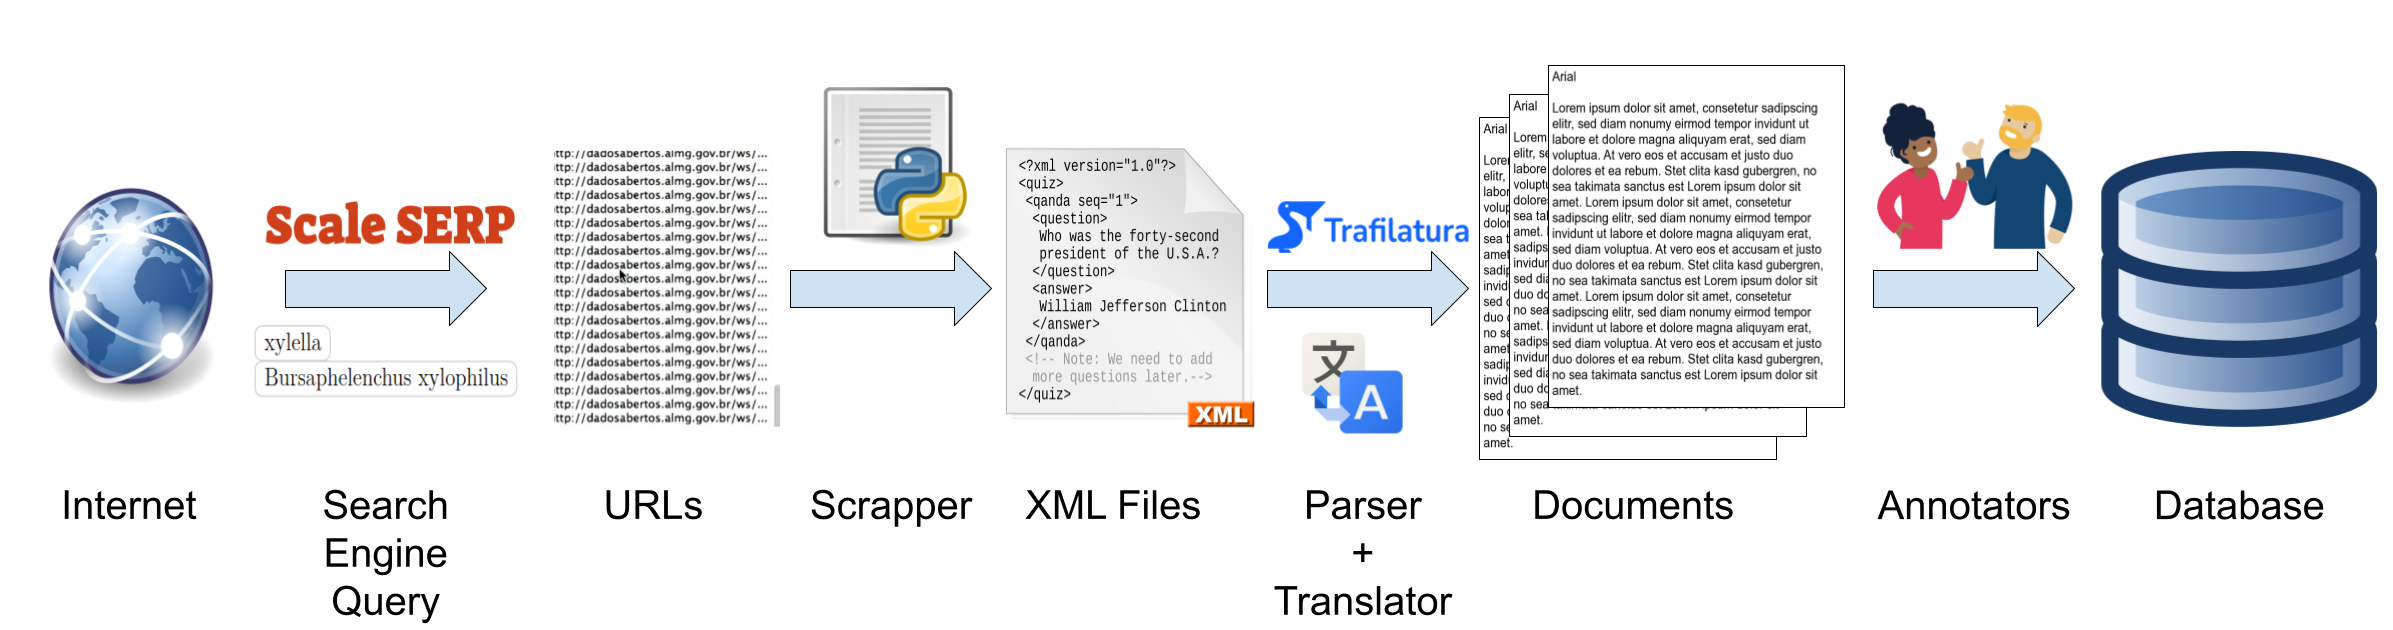
\includegraphics[width=\textwidth]{Figures/04/04_vsi_dataset_collection.png}
    \caption{\VSI{} Data Collection Pipeline}
    \label{fig:04_vsi_data_collection_pipeline}
\end{figure}


The main tool for collecting documents is the web scrapping tool \emph{ScaleSERP}\footnote{\url{https://www.scaleserp.com/}}. Every week, several queries are sent to various services, including the Google Search Engine, using the keywords and key phrases related to pathogens of interest (Table \ref{tab:04_query_keywords}).%, using a Python script. 
%The results are then fed to the text-mining tool \emph{PADI-Web} \myparencite{padiweb3}, in order to retrieve information about the document's source, publication date, entities mentioned, locations and more. After extraction, this data is stored in a database and subsequently analysed by the \gls{vsi} experts to assess their relevance for monitoring. 


As part of the \gls{vsi} pipeline, shown in Figure \ref{fig:04_vsi_data_collection_pipeline}, the websites corresponding to the URLs obtained from \emph{ScaleSERP} are downloaded using a Python script. 
For each website, its source (in HTML) is downloaded, and the tool \trafilatura{} \myparencite{barbaresi-2021-trafilatura} parses it to XML/TEI, while attempting to discard ``non-contents", such as menus, headings, ads, etc.
Then, \trafilatura{} takes the XML/TEI and attempts to extract a title and  an abstract from the metadata\footnote{The title and the abstract are extracted from the \texttt{metadata.title} and \texttt{metadata.description} fields, respectively.} and the full text from the XML body.

%Then, they are scrapped using the tool \trafilatura{}.
%the documents  are scrapped using the tool \trafilatura{} \myparencite{barbaresi-2021-trafilatura}, which attempts to extract a title, an abstract, the full text, and other data from the websites.
%Specifically, for a website, \trafilatura{} scrapes the HTML content and parses it into XML. The tool then extracts the title and abstract from the XML metadata\footnote{The title and the abstract are extracted from the \texttt{metadata.title} and \texttt{metadata.description} fields, respectively.} and the full text from the XML body.

Given that these articles are extracted from public websites, they remain in their original language. The Google Translate API is used to assist the annotators with foreign-language articles. This API also automatically detects the document's language.
Due to budget constraints, only the \trafilaturaTitle{} is translated into English.


%Given that these articles come from public websites, all the content is in its original language.
%In order to help the annotators make a decision when encountering an article in a foreign language, and due to budget limitations, only the title is translated to English, using the Google Translate API, which also provides an automatically detected language for the document. 

Since documents are added each week, the \gls{vsi} database is in constant construction. 
For our work, we utilized with the documents collected from the 11th of July 2022 to the 16th of April 2023, that is, the data collected over 39 weeks, comprising approximately 35,000 documents, which corresponds to more than 800 documents per week. We focus on a subset of the \VSI{} database, specifically its textual data, to obtain the \VSI{} dataset  (Table \ref{tab:04_pesv_sources of content}).

\input{Tables/04/Sources_of_content_trafilatura_google_translate}



% %%%%%%%%%%%%%%%%%%%%%%%%%%%%%%%%%%%%%%%%%%%%%%%%%%%%%%%%%%%%%%%%%%%%%%%%%%%%%%%%%%%%%%
\customHeader{1}{Dataset Annotation}
\label{vsi_data_annotation}

\putInBox{
There are four \gls{vsi} experts dedicated to annotating the dataset.
Regrettably, while constructing the dataset, there was no record maintained to track the identity of the annotator responsible for labelling each document. For this reason, we are not able to provide any inter-annotator agreement measures on this dataset \myparencite{agreement_measures}.
}



%\begin{itemize}
%    \item \todo{add names of \gls{vsi} experts}
%    \item \todo{add names of \gls{vsi} experts}
%    \item \todo{add names of \gls{vsi} experts}
%    \item \todo{add names of \gls{vsi} experts}
%\end{itemize}


%After obtaining results from the Google Search, the \gls{vsi} experts are presented with the URL of a document, which they manually open and proceed to read. Using the interface in Figure \ref{fig:04_pesv_interface_1}, they fill out the fields \emph{Titre} (title), \emph{Auteurs} (authors), \emph{Organism nuisible} (pathogen), \emph{Sujet} (subject), \emph{Fiabilité} (reliability), etc. 

For annotation, the results of the \gls{vsi} pipeline mentioned above are shared with the \gls{vsi} experts. They utilize the interface shown in Figure \ref{fig:04_pesv_interface_1} to inspect the results for various fields, including the \emph{Date de publication} (publication date), \emph{Auteurs} (authors), \emph{Organism nuisible} (pathogen), etc. Additionally, they manually input information in other fields such as \emph{Sujet} (subject), \emph{Fiabilité} (reliability), and come up with a \emph{Titre} (title).
It is important to note that the title written by the \gls{vsi} experts is usually different from the one extracted by \trafilatura{} (for example, 
%they may include different characters
the wording may vary). 
%Other fields, like \emph{Date de publication} (publication date) and \emph{Lien} (link) are filled automatically.

After inspection, we found that that annotators exclusively provide titles for articles they find relevant, that is, there are no titles for irrelevant articles. Since our objective is to automate the process of identifying relevant articles, we disregard the titles provided by the annotators. Instead, we rely solely on the titles generated by \trafilatura{} and Google Translate, which are stored even in the case of the documents being rejected.

Special attention must be given to the \emph{Sujet} (subject), as this field will be crucial for preprocessing the dataset (see \headerName{} \ref{vsi_resolving_inconsistencies}).

\putInBox{
%As part of their monitoring mission, the \gls{pesv} Platform surveys any health risk or plant health phenomenon that has or may have an impact on agriculture. 
When the \gls{vsi} experts encounter an event that catches their attention (that is, that they consider \textbf{relevant}), they assign a \textbf{subject} to the respective document and utilize the interface presented in Figure \ref{fig:04_pesv_interface_2} to allocate a subject ID and description to the document.
Each subject corresponds to a specific health risk event that was reported during the weeks before the experts reviewed the documents.
It is possible for multiple documents to share the same subject. In the case of documents considered \textbf{irrelevant} to the monitoring of plant health, the subject field for the document is left empty.
}

Subsequently, after a document is deemed relevant by the \gls{vsi} experts, it is officially published in the bulletin of the  \gls{pesv} Platform\footnote{\url{https://plateforme-esv.fr/bulletins_et_points_sur_VSI}} and can be accessed through the \gls{vsi} Document Search Engine\footnote{\url{https://plateforme-esv.fr/moteur-de-recherche-vsi}}. Some sample entries containing all sources of content can be found in Table \ref{tab:04_sample_entries_vsi}.


\input{Tables/04/Sample_entries}


\begin{landscape}
    \begin{figure}[ht]
        \centering
        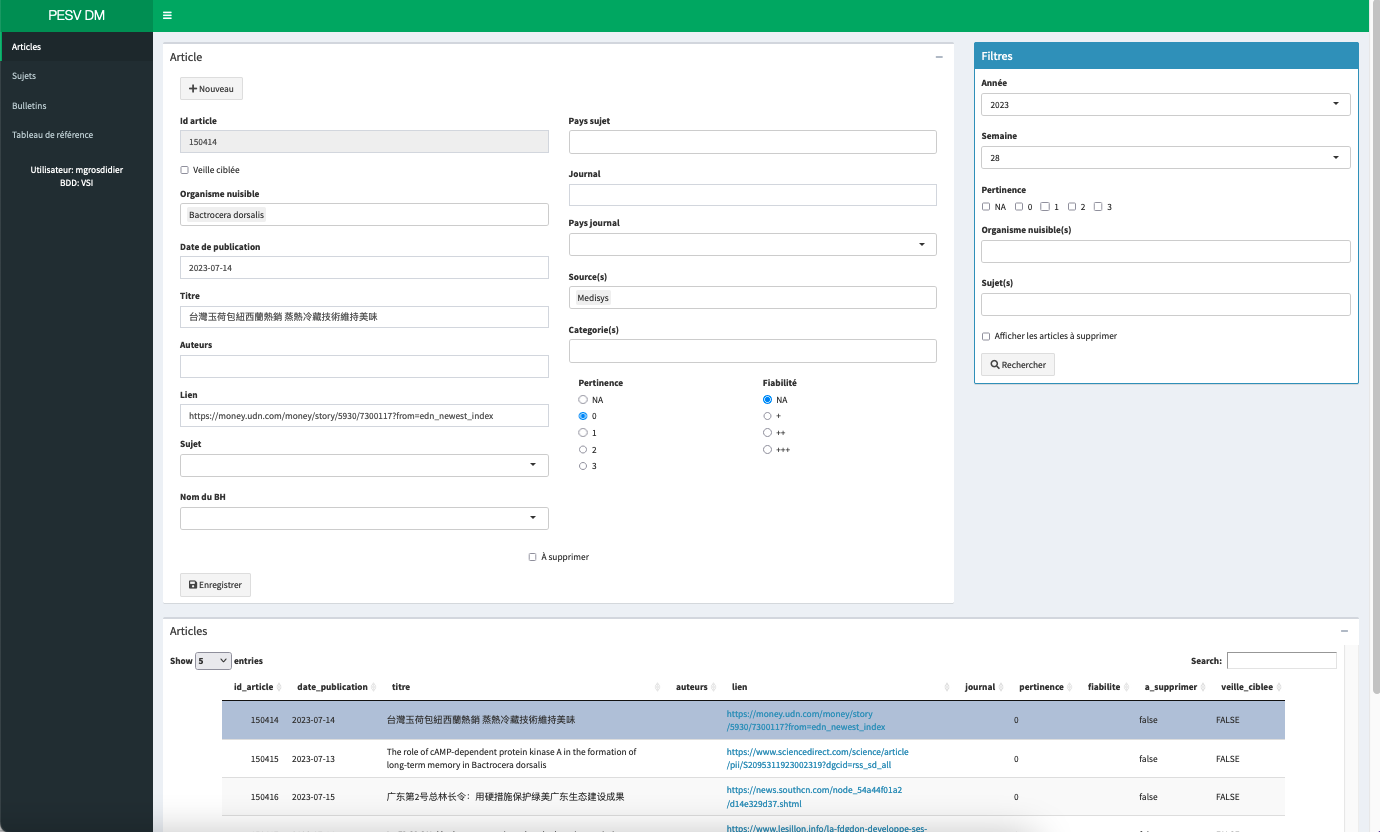
\includegraphics[width=1.20\textwidth]{Figures/04/PESV_interface_1.png}
        \caption{\VSI{} Annotation Interface for Articles}
        \label{fig:04_pesv_interface_1}
    \end{figure}
\end{landscape}

\begin{landscape}
    \begin{figure}[ht]
        \centering
        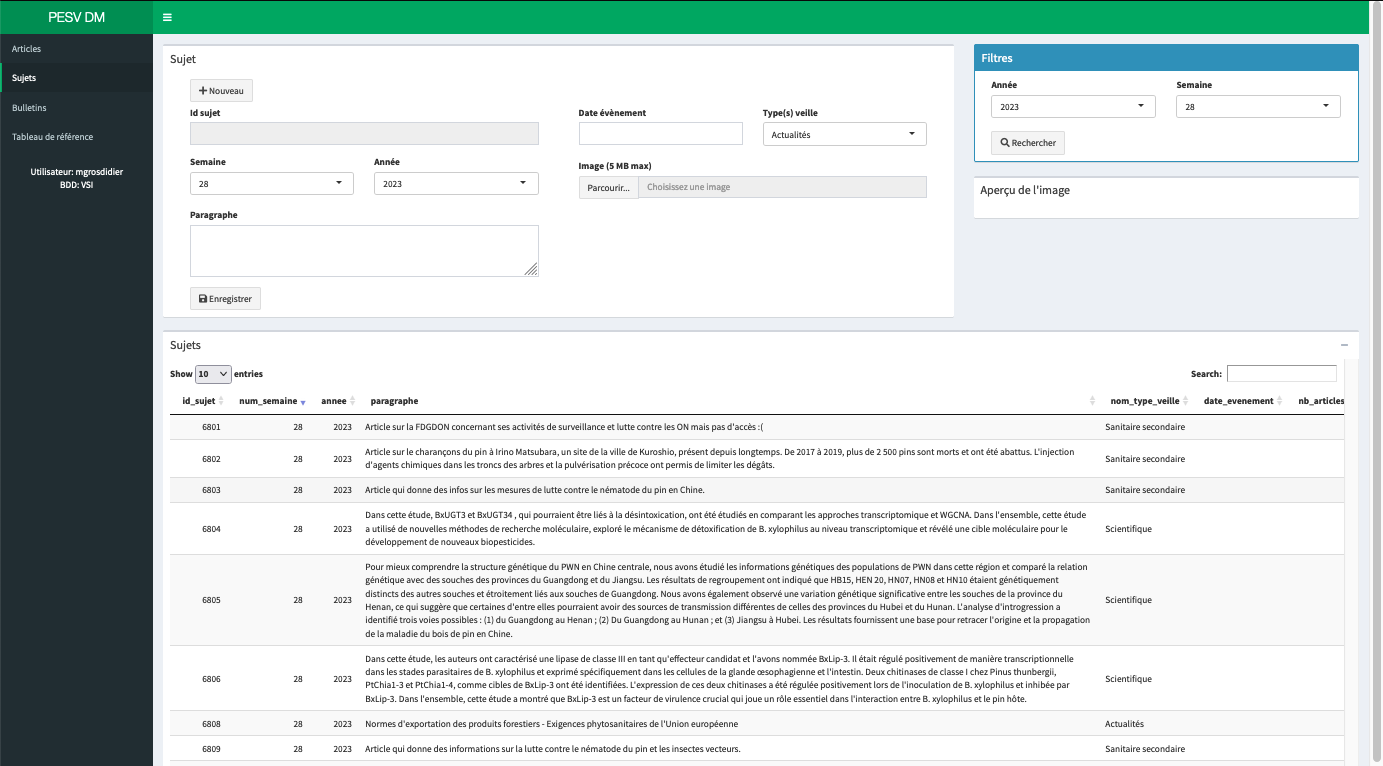
\includegraphics[width=1.20\textwidth]{Figures/04/PESV_interface_2.png}
        \caption{\VSI{} Annotation Interface for Subjects}
        \label{fig:04_pesv_interface_2}
    \end{figure}
\end{landscape}


% %%%%%%%%%%%%%%%%%%%%%%%%%%%%%%%%%%%%%%%%%%%%%%%%%%%%%%%%%%%%%%%%%%%%%%%%%%%%%%%%%%%%%%
\customHeader{1}{Dataset Stastitics}
\label{vsi_data_statistics}

There are 34,587 entries in the dataset, out of which 3,715 have an assigned subject and 30,872 do not, producing a highly unbalanced dataset (Figure \ref{fig:04_naive_positives_and_negatives}). 

\begin{figure}
    \centering
    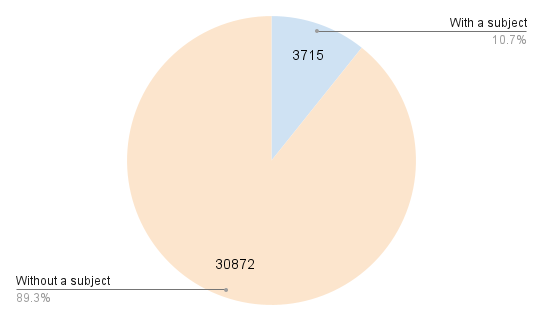
\includegraphics[width=0.75\textwidth]{Figures/04/naive_positives_and_negatives_chart.png}
    \caption{Distribution of subjects in the \VSI{} dataset without preprocessing}
    \label{fig:04_naive_positives_and_negatives}
\end{figure}

The language automatically detected by the Google Translate API on the \trafilaturaTitle{} can be used to approximately study the distribution of the entries in the dataset. In Figure \ref{fig:04_vsi_language_distribution} it can be seen that around one third of the entries are in English, followed by Italian, Spanish, and French. There is a considerable amount of failed translation attempts, for around one fifth of the entries. The complete data on documents per language is available in Appendix \ref{appendix01:vsi_language_distribution}.
 
\begin{figure}
    \centering
    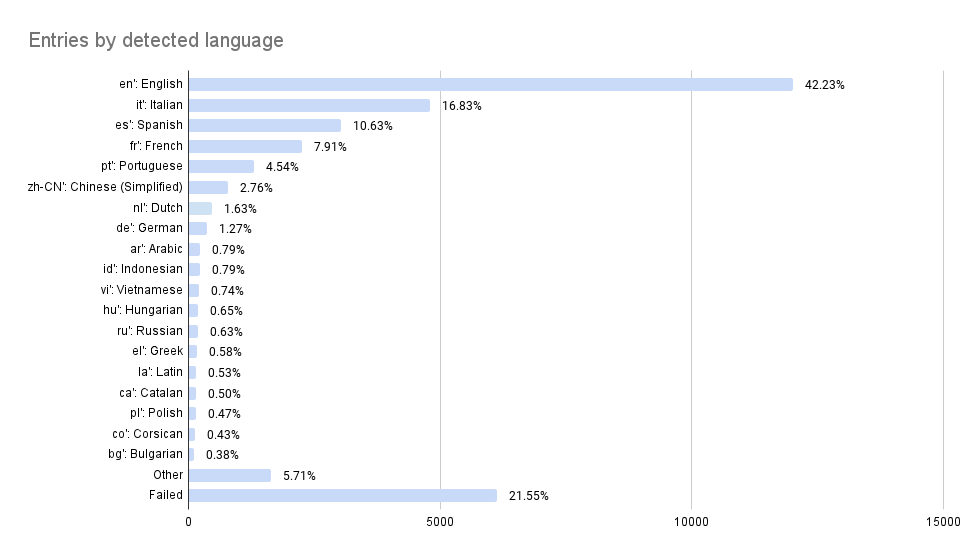
\includegraphics[width=\textwidth]{Figures/04/Entries by detected language.png}
    \caption{Language distribution of entries in the \VSI{} dataset}
    \label{fig:04_vsi_language_distribution}
\end{figure}

The presence of some Latin documents is surprising. Upon inspecting the data, we discovered that this occurrence was due to scrapped \trafilaturaTitle{}s with several scientific names (Table \ref{tab:appendix01:latin_entries} in the Appendix).

Often, the \trafilatura{} scrapper is not able to retrieve content for the \trafilaturaTitle{}, \trafilaturaAbstract{}, and \trafilaturaFulltext{} of a website, or the Google Translate API fails. Thus, there are several entries without content for all fields. If we check the unique entries for each source of content, we can see that there are numerous duplicate entries, since there are at least around 20,000 unique entries per source of content (Figure \ref{fig:04_unique_entries_vsi}).

\begin{figure}
    \centering
    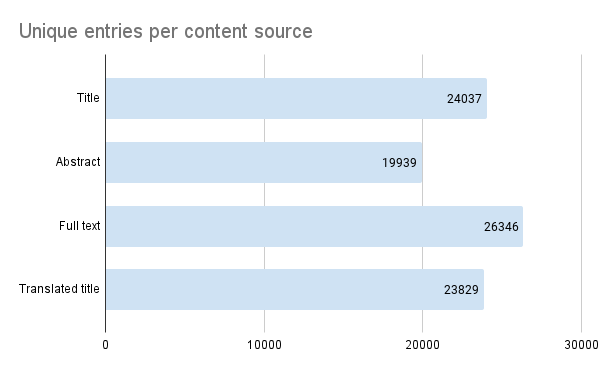
\includegraphics[width=0.50\textwidth]{Figures/04/Unique entries per content source.png}
    \caption{Unique entries per source of content in the \VSI{} dataset}
    \label{fig:04_unique_entries_vsi}
\end{figure}

As the\translationTitle{} is derived from the \translationTitle{}, and due to the possibility of failure in the Google Translate API, the number of unique entries for the \translationTitle{} is lower than that for the \trafilaturaTitle{}.
%As one would expect, there are fewer unique entries for the \translationTitle{} as there are for the \trafilaturaTitle{}. 
At the same time, the \trafilaturaAbstract{} field has fewer unique entries than all the other \contentType{}s, while the \trafilaturaFulltext{} has the most. This may be explained by the fact that, usually, the creators of a website omit filling the metadata, and when they do, they frequently include only a title and not a description, while most times, the body of the website will be available. 

Using naive tokenization (splitting on whitespace), we can study the distribution of the tokens for all sources of content. In the histograms in Figure \ref{fig:04_vsi_token_distribution} the longest documents have been grouped together to facilitate plotting \footnote{This explains the long bars at the end of the right tails of the histograms.}. As one can see, the \trafilaturaTitle{} and \translationTitle{} have a very similar distribution, both are shorter than the \trafilaturaAbstract{}, while the content from the \trafilaturaFulltext{} is the longest.

\begin{figure}[ht]
    \centering
    \subfigure[\trafilaturaTitle{}]{
        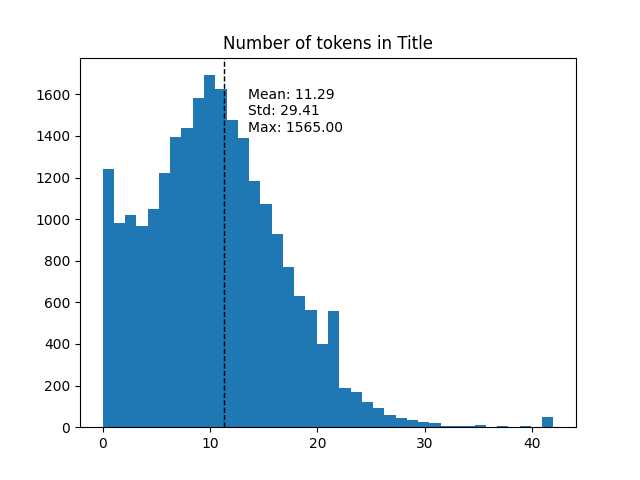
\includegraphics[width=0.45\textwidth]{Figures/04/Histograms/length histogram parsed_trafilatura_title.png}
        %\label{fig:image1}
    }
    \hfill
    \subfigure[\trafilaturaAbstract{}]{
        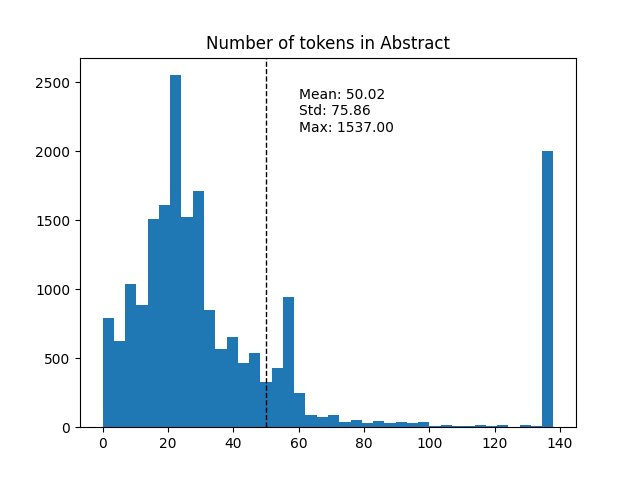
\includegraphics[width=0.45\textwidth]{Figures/04/Histograms/length histogram parsed_trafilatura_abstract.png}
        %\label{fig:image2}
    }
    
    \subfigure[\trafilaturaFulltext{}]{
        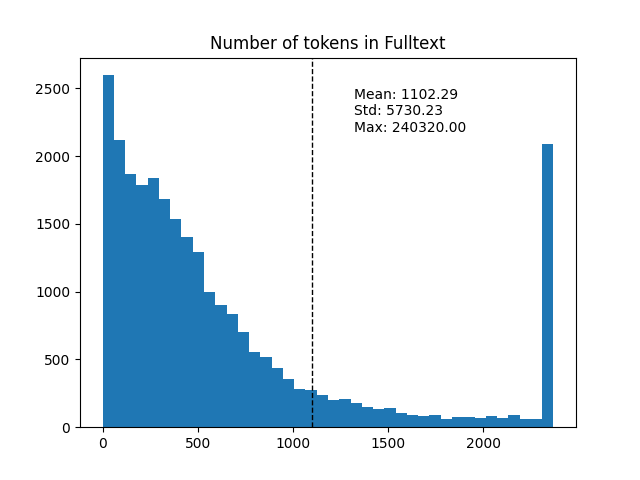
\includegraphics[width=0.45\textwidth]{Figures/04/Histograms/length histogram parsed_trafilatura_fulltext.png}
        %\label{fig:image3}
    }
    \hfill
    \subfigure[\translationTitle{}]{
        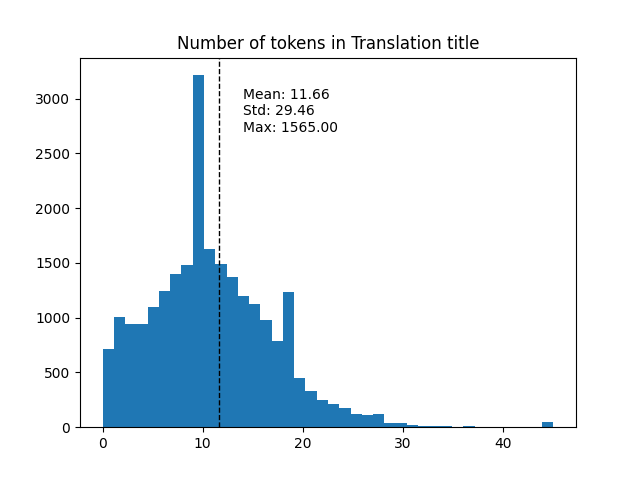
\includegraphics[width=0.45\textwidth]{Figures/04/Histograms/length histogram translation_title.png}
        %\label{fig:image4}
    }
    
    \caption{
    Length (in n. of tokens) of the \contentType{}s in the \VSI{} dataset
    }
    \label{fig:04_vsi_token_distribution}
\end{figure}







% %%%%%%%%%%%%%%%%%%%%%%%%%%%%%%%%%%%%%%%%%%%%%%%%%%%%%%%%%%%%%%%%%%%%%%%%%%%%%%%%%%%%%%
\customHeader{1}{Dataset Issues}
\label{vsi_data_issues}


Upon examining the data, we encountered numerous issues that we proceed to describe and which will be addressed during preprocessing (\headerName{} \ref{vsi_preprocessing}).


\customHeader{2}{Duplicate Entries}
\label{vsi_issues_duplicates}
\ \\

As mentioned in \headerName{} \ref{vsi_data_statistics}, there are some duplicate entries in the dataset (Figure \ref{fig:04_naive_positives_and_negatives} VS Figure \ref{fig:04_unique_entries_vsi}). According to the \gls{vsi} experts, often the Google Search for a query will return the same results from one week to the next, and this introduces duplicate entries.
 


\customHeader{2}{Scrapping Failures}
\label{vsi_issues_error_messages}
\ \\

On some instances, the \trafilatura{} scrapper either fails or is blocked by website servers that do not allow bots. This introduces error messages to the dataset, some samples of which can be seen in Table \ref{tab:04_error_messages}.

\input{Tables/04/Error_messages}



\customHeader{2}{Scrapping errors}
\label{vsi_issues_scrapping_errors}
\ \\

In some other instances, the web scraper successfully extracts content from the website, but the parsing algorithm performs poorly, retrieving only the headers or the website's name (Tables \ref{tab:04_headers} and \ref{tab:04_website_names}).

\input{Tables/04/Headers_and_websites}

This type of scrapping error introduces inconsistencies into the \VSI{} dataset, as multiple documents end up having the same text for several \contentType{}s, as in Table \ref{tab:04_xmol_inconsistencies}\footnote{\href{https://www.x-mol.com/}{X-MOL} is a Chinese search engine for scholars.}.

%This introduces inconsistencies into the \VSI{} dataset. In cases where multiple documents originate from the same problematic website, the original content is lost, and we encounter entries that contain identical text but carry different assigned subjects, as in Table \ref{tab:04_xmol_inconsistencies}\footnote{\href{https://www.x-mol.com/}{X-MOL} is a Chinese search engine for scholars.}.




\input{Tables/04/X-MOL_problem}




\customHeader{2}{Data Noise}
\label{vsi_issues_data_noise}
\ \\

Even in those cases when \trafilatura{} is able to retrieve content from the website, there are some expected types of noise in the data, considering it comes from the internet.
Namely, the following  (Table \ref{tab:04_noise}) :
\begin{itemize}
    \item URLs
    \item HTML Tags
    \item Emojis
    \item Encoding errors
    \item Generic noise (different quotation or division characters, strings containing only dates, etc\ldots)
\end{itemize}




% endings - pubmed
% URLs, tags, emojis


\input{Tables/04/Noise}


Furthermore, there exists a source of noise that may not be immediately apparent: occasionally, the content concludes with the website's name, leading to different entries that vary by only a few tokens as a suffix (Table \ref{tab:04_website_names_as_suffixes}).

\input{Tables/04/Similar_entries}


\customHeader{2}{Annotation Inconsistencies}
\label{vsi_issues_annotation_inconsistencies}
\ \\

Finally, human error also introduces inconsistencies into the \VSI{} dataset. In some cases, there are entries with the exact same content, with different or no assigned subjects (Table \ref{tab:04_annotation_inconsistencies}). After consulting with the \gls{vsi} experts, they explained that this is due to two factors:

\begin{itemize}
    \item Different annotators labeling the same content.
    \item After a subject loses relevance (see \headerName{} \ref{vsi_data_collection}), the annotators usually ignore articles related to it, which is effectively equivalent to assigning no subject.
\end{itemize}


\input{Tables/04/Annotation_inconsistencies}


\putInBox{
Due to all the issues mentioned, one must take the statistics in \headerName{} \ref{vsi_data_statistics} with a grain of salt. In particular, naively checking the entries for the presence of an assigned subject (as in Figure \ref{fig:04_naive_positives_and_negatives}) may lead to very similar or exactly equal content labelled in two different categories, thus rendering the classification task significantly more challenging. These issues will addressed during preprocessing (\headerName{} \ref{vsi_preprocessing}).
}



% making sure to print all tables and figures 
\clearpage
\customHeader{1}{\Sanba{} Dataset}
\label{sanba_dataset}
\customHeader{0}{Preprocessing the \VSI{} dataset}
\label{vsi_preprocessing}


%\customHeader{0}{Preprocessing}
%\label{preprocessing}

In this \headerName{}, we outline the approaches taken to resolve the challenges found in the \gls{vsi} Dataset. After reviewing the problems described in \headerName{} \ref{vsi_data_issues}, we adopted various tactics to achieve a preprocessed dataset suitable for \textclassification{}.


%\customHeader{1}{Preprocessing the \VSI{} dataset}
%\label{vsi_preprocessing}



% %%%%%%%%%%%%%%%%%%%%%%%%%%%%%%%%%%%%%%%%%%%%%%%%%%%%%%%%%%%%%%%%%%%%%%%%%%%%%%%%%%%%%%
\customHeader{1}{Leveraging Keywords}
\label{vsi_leveraging_keywords}

Leveraging the available keywords and key phrases used for the Search Engine queries used to construct the dataset (Table \ref{tab:04_query_keywords}), we obtained four more sources of content. 

\begin{figure}
    \centering
    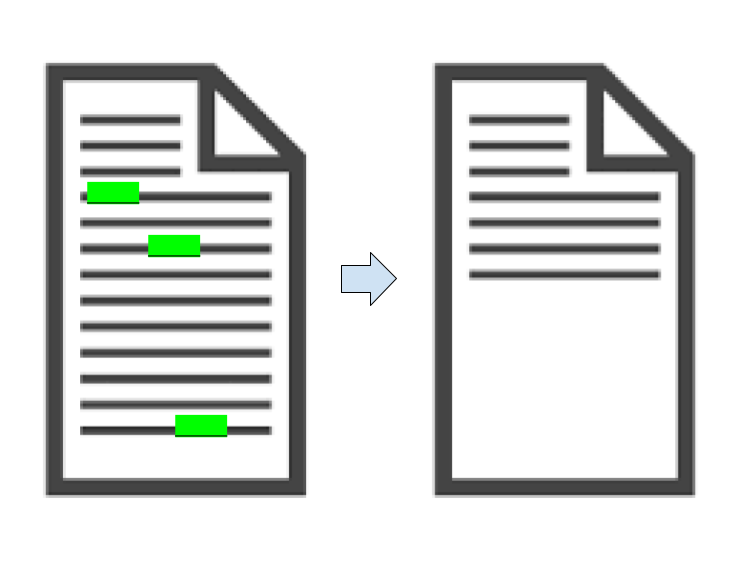
\includegraphics[width=0.5\textwidth]{Figures/05/05_keyphrase_extraction.png}
    \caption{Extracting phrases with Keywords}
    \label{fig:05_keyphrase_extraction}
\end{figure}

%We opted to extract sentences containing keywords or key phrases from the content. 
Using the Python package \texttt{NLTK} \myparencite{nltk}, we divided each document into phrases and selected those containing at least one of the keywords or key phrases. This process was carried out for both the \trafilaturaAbstract{} and \trafilaturaFulltext{} sources of content (Figure \ref{fig:05_keyphrase_extraction}). 
However, considering the diverse range of languages in the documents, it was not always apparent whether we should discard the content entirely or retain it. For example, even if the keyword is not present in the text, maybe its translation is; or we could be facing a language written in a non-Latin script.
Consequently, we pursued two different approaches: in one case, we discarded the original content (O.C.), and in the other, we retained it, resulting in four new sources of content (Table \ref{tab:05_pesv_sources of content after preprocessing}).

\input{Tables/05/Sources_of_content_after_preprocessing}


Figure \ref{fig:05_unique_entries_keyphrases_vsi} offers a comparison of the number of unique entries per content source. In both cases, keeping only the phrases containing keywords dramatically reduces the size of the data, especially for the \trafilaturaAbstract{}. Possible reasons for this will be explained in \headerName{} \ref{vsi_data_cleaning}. Note that, in the case of keeping the original content, there are slightly fewer unique entries for both the \trafilaturaAbstract{} and the \trafilaturaFulltext{} ($19,939-19,798 = 141$ and $26,346-24,447=1,899$, respectively). This may be explained by the fact that some data noise may be removed by the sentence extraction process, especially those cases where several entries differ by a small amount of tokens (see Table \ref{tab:04_website_names_as_suffixes}).

\begin{figure}
    \centering
    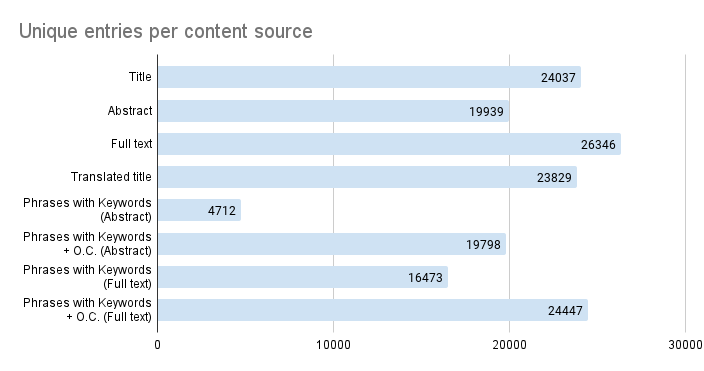
\includegraphics[width=0.750\textwidth]{Figures/05/Unique entries per content source_keyphrases.png}
    \caption{Unique entries per source of content in the \VSI{} dataset}
    \label{fig:05_unique_entries_keyphrases_vsi}
\end{figure}


% %%%%%%%%%%%%%%%%%%%%%%%%%%%%%%%%%%%%%%%%%%%%%%%%%%%%%%%%%%%%%%%%%%%%%%%%%%%%%%%%%%%%%%
\customHeader{1}{Data Cleaning}
\label{vsi_data_cleaning}



\customHeader{2}{Noise Removal}
\label{vsi_string_cleaning}

To address the text noise mentioned in \headerName{} \ref{vsi_issues_data_noise}, we use regular expressions to:

\begin{enumerate}
    \item Remove characters not in any human alphabet. This handles encoding errors.
    \item Remove emojis, URLs, HTML tags, hours, dates, extra white spaces.
    \item Remove punctuation at beginning and end of the string.
    \item Remove digits at beginning and end of the string.
    \item Standardize quotation characters into the ASCII simple quotation character (').
    \item Standardize hyphen-like characters into the ASCII hyphen (-).
    \item Remove sentence suffixes that may be the name of the website, by deleting short text ($\leq 3$ tokens) that follow an ASCII hyphen or bar (|) near the end of the string.
\end{enumerate}

See Table \ref{appendix02:tab:pesv_string_cleaning_regex} in the \appendixname{} for some examples of the regular expressions used to clean the multilingual strings. Figure \ref{fig:05_multilingual_string_cleaning} shows the effect of string cleaning on an example text.

\begin{figure}
    \centering
    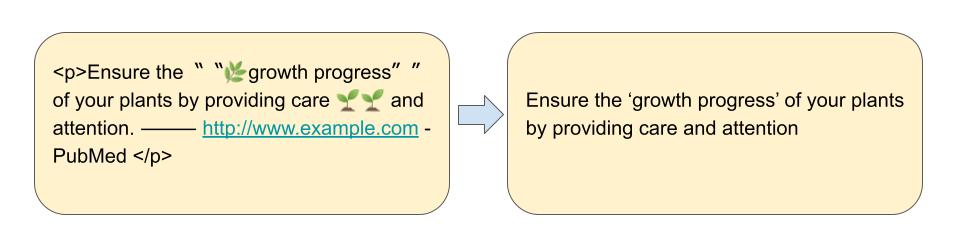
\includegraphics[width=\textwidth]{Figures/05/05_multilingual_string_cleaning.png}
    \caption{Removing noise from multilingual strings}
    \label{fig:05_multilingual_string_cleaning}
\end{figure}


\customHeader{2}{Deleting Error Messages}
\label{vsi_deleting_error_messages}

Fortunately, error messages in the dataset are very consistent. Given that they do not provide information on the relevance of a document, we may delete them using regular expressions. See Table \ref{appendix02:tab:error_messages} in the \appendixname{} for some examples of the regular expressions used to remove the error messages. 

\input{Tables/05/Error_count}

In Table \ref{tab:05_vsi_error_message_count}, we present the number of error messages identified using our regular expressions. Notably, the proportion of error messages generally hovers around one-fifth of all entries. In $18.50\%\ (\approx 20\%)$ of cases \trafilatura{} completely fails to obtain any content from the website. This proportion almost doubles ($36.50\approx 40\%$) for the \trafilaturaAbstract{}. This discrepancy in the \trafilaturaAbstract{} could be attributed to the common occurrence of missing metadata, as discussed in \headerName{} \ref{vsi_data_statistics}.


\customHeader{2}{Handling scrapping errors}
\label{05_vsi_handling_scrapping_errors}
% first attempt with title names regex. failed ~ 300 docs fewer
% second attempt: by length


In order to handle scraping errors from \trafilatura{}, such as obtaining the name of the website or certain HTML headers, our first approach was to use regular expressions to filter them out. After removing the error messages from all sources of content, we proceeded to count the occurrences of each entry and ranked them in descending order. Given that our dataset contains approximately 35,000 documents, we focused on entries that appeared at least twice.

Although we attempted to identify common patterns and create regular expressions to match frequent entries, this approach proved unsuccessful. It only filtered around 500 unique entries, accounting for a mere $2\%$ of all unique entries in the best case (\trafilaturaAbstract{}). Consequently, it became apparent that several scraping errors likely appeared only once in the dataset, rendering our previous strategy ineffective.

Nevertheless, along this examination, we noticed that scraping errors tend to be short in length (see Tables \ref{tab:04_headers} and \ref{tab:04_website_names}). As a result, we devised a new filtering strategy based on the length of the entries. However, simply counting naive tokens was insufficient, as languages like Chinese often lack whitespace in their text. Therefore, we needed a more robust algorithm to determine when a string is considered suspiciously ``too short."

Our heuristic to filter by length consists in:

\begin{enumerate}
    \item First, the string is split on white spaces.
    \item Then, if there is only one token, and the string has less than 20 characters, it is considered ``too short".
    \item Next, if there are less than four tokens, the string is considered ``too short"
    \item Finally, in all other cases, we keep the string.
\end{enumerate}

\input{Tables/05/Short_document_count}


Upon removing error messages, we observed that parsing errors occur in entries for the \trafilaturaTitle{} and the \translationTitle{} approximately 1 in 7 times ($\approx 16\% $), as can be seen in Table \ref{tab:05_vsi_short_document_count}. The \trafilaturaAbstract{} and \trafilaturaFulltext{} are rarely short ($\leq 3\% $), and very few entries have more than one content source that is too brief ($\leq 3\% $).


% %%%%%%%%%%%%%%%%%%%%%%%%%%%%%%%%%%%%%%%%%%%%%%%%%%%%%%%%%%%%%%%%%%%%%%%%%%%%%%%%%%%%%%
\customHeader{1}{Resolving Inconsistencies and Duplicate Documents}
\label{vsi_resolving_inconsistencies}

The initial preprocessing steps focused solely on cleaning the textual content of the dataset. Now, our attention turns to addressing the labeling challenges, specifically, instances where entries have identical content but differ in subject assignment or lack a subject (as in Tables \ref{tab:04_xmol_inconsistencies} and \ref{tab:04_annotation_inconsistencies}).

Considering our main goal is to automate the identification of articles relevant to the \gls{vsi} experts, where subject assignment signifies their interest, we propose the following strategy:

\putInBox{
For each of the eight content sources, we group the dataset based on the text content. If a particular text has been assigned a subject at least once, we categorize it as \textbf{relevant}. Conversely, if no subject has been assigned to a text, we consider it \textbf{irrelevant}.
}

We believe this strategy reflects the intention of the annotators as they labeled the documents (see \headerName{} \ref{vsi_data_annotation}). Additionally, by design, this strategy eliminates duplicate content. Table \ref{tab:determining_relevance} illustrates this process for the content from the \trafilaturaTitle{}.

\input{Tables/05/Strategy_for_labelling}


% %%%%%%%%%%%%%%%%%%%%%%%%%%%%%%%%%%%%%%%%%%%%%%%%%%%%%%%%%%%%%%%%%%%%%%%%%%%%%%%%%%%%%%
\clearpage
\customHeader{1}{Preprocessing Results}
\label{vsi_results_of_preprocessing}

In this section, we present the outcomes of our preprocessing techniques, yielding refined datasets suitable for text classification. Additional numerical results can be found in \appendixname{} \ref{appendix03:vsi_preprocessing results}.

Figure \ref{fig:05_unique_entries_after_preprocessing} demonstrates that preprocessing leads to a reduction in the number of unique entries. For the majority of \contentType{}s, approximately 5 out of 6 unique entries are retained after the filtering process ($\approx 85\%$), except for the \trafilaturaTitle{} and \trafilaturaAbstract{}, where approximately 4 out of 6 unique entries are preserved ($\approx 67\%$).


\begin{figure}
    \centering
    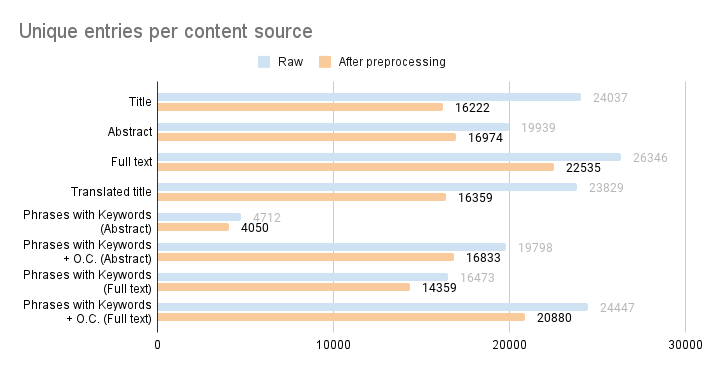
\includegraphics[width=0.75\textwidth]{Figures/05/Preprocessing_Unique entries per content source.png}
    \caption{Unique Entries per content source before and after preprocessing}
    \label{fig:05_unique_entries_after_preprocessing}
\end{figure}

\input{Tables/05/Unique_entries_after_preprocessing}


Regarding the average token count of the content, the histograms in Figure \ref{fig:05_vsi_token_distribution_after_preprocessing} show that distributions across the four original \contentType{}s align with the original observations in Figure \ref{fig:04_vsi_token_distribution}. The same trend is observed for the \keyphrases{} as well. Upon comparing the means before and after preprocessing (Table \ref{tab:05_vsi_mean_tokens_before_after_preprocessing}), we observe that the means are higher for all the original content sources, except for the \trafilaturaFulltext{}.

The higher means can be attributed to the filtering of error messages, which tend to be short in length, and short entries that may correspond to scrapping errors. As for the \trafilaturaFulltext{}, upon closer inspection of the filtered-out \emph{long} texts identified as error messages, it was observed that they often pertain to topics such as website cookies or terms and conditions. These texts tend to be quite lengthy and are not typically found in website metadata (from where the \trafilaturaTitle{} and the \trafilaturaAbstract{} are extracted). This observation explains the lower mean for the \trafilaturaFulltext{} after preprocessing, which we interpret as a positive indication of our filtering approach.

When analyzing the \keyphrases{}, a significant decrease in the mean is noted, particularly for the \keyphrases{} extracted from the \trafilaturaFulltext{}. This reduction can be attributed to the fact that only a few sentences in an article usually contain the exact keywords used for locating them through a  Search Engine. Consequently, after preprocessing, the mean of the \keyphrases{} decreases substantially when compared to their original sources.

Overall, these observations highlight the effectiveness of our preprocessing in removing undesirable content while retaining relevant information.





\begin{figure}[ht]
    \centering
    \subfigure[\trafilaturaTitle{}]{
        \begin{adjustbox}{max height=0.18\textheight}
            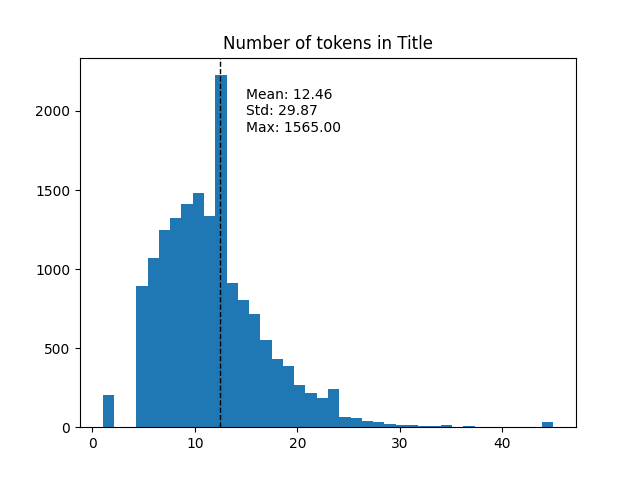
\includegraphics[width=0.45\textwidth]{Figures/05/Histograms/preprocessing length histogram parsed_trafilatura_title.png}
        \end{adjustbox}
        %\label{fig:image1}
    }
    \hfill
    \subfigure[\trafilaturaAbstract{}]{
            \begin{adjustbox}{max height=0.18\textheight}
            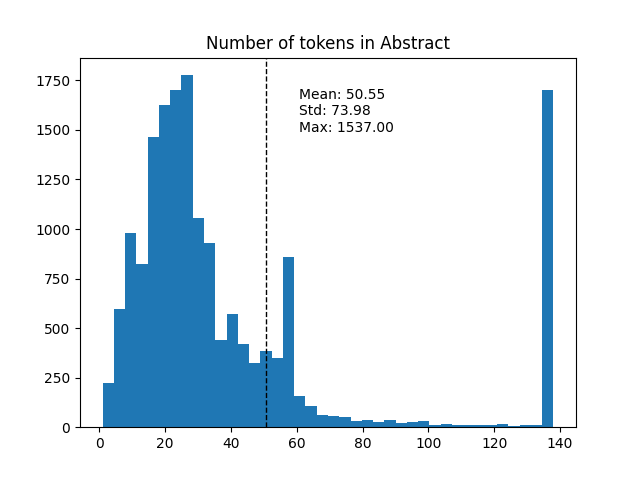
\includegraphics[width=0.45\textwidth]{Figures/05/Histograms/preprocessing length histogram parsed_trafilatura_abstract.png}
        \end{adjustbox}

        %\label{fig:image2}
    }
    
    \subfigure[\trafilaturaFulltext{}]{
        \begin{adjustbox}{max height=0.18\textheight}
          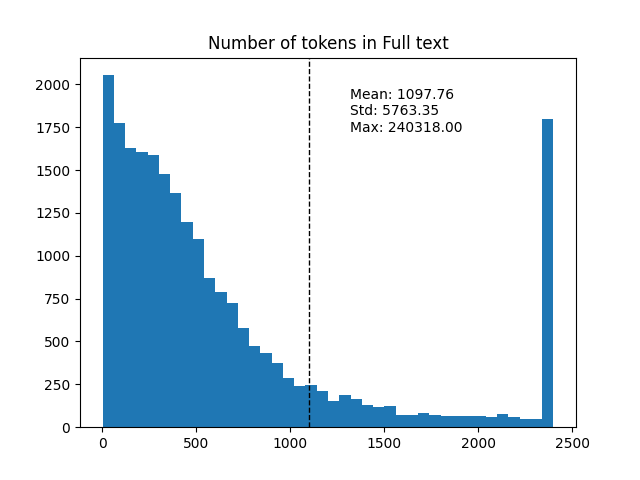
\includegraphics[width=0.45\textwidth]{Figures/05/Histograms/preprocessing length histogram parsed_trafilatura_fulltext.png}
        \end{adjustbox}
        %\label{fig:image3}
    }
    \hfill
    \subfigure[\translationTitle{}]{
            \begin{adjustbox}{max height=0.18\textheight}
                    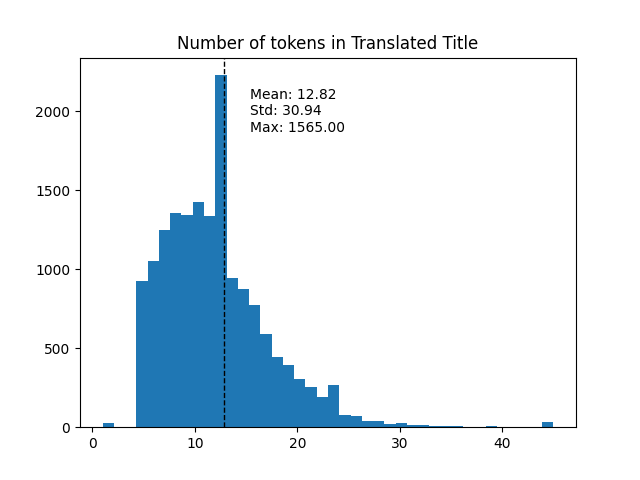
\includegraphics[width=0.45\textwidth]{Figures/05/Histograms/preprocessing length histogram translation_title.png}
        \end{adjustbox}
        %\label{fig:image4}
    }
    
    
    %%
    \subfigure[\keyphrasesAbstractOnly{}]{
        \begin{adjustbox}{max height=0.18\textheight}
            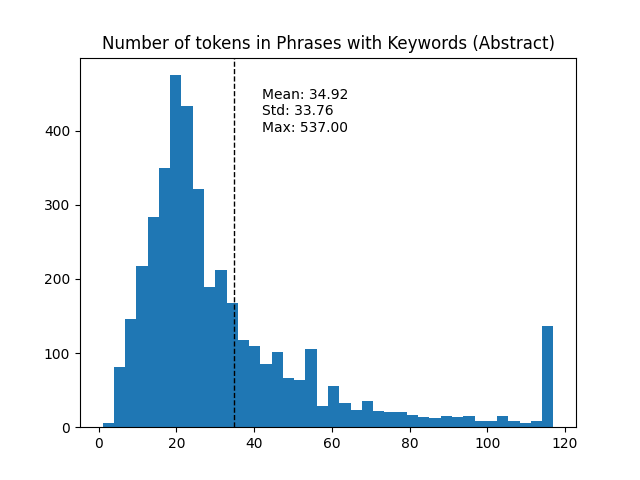
\includegraphics[width=0.45\textwidth]{Figures/05/Histograms/preprocessing length histogram sentence_with_keywords_parsed_trafilatura_abstract_only_relevant_sentences.png}
        \end{adjustbox}
        
        %\label{fig:image2}
    }
    \hfill
    \subfigure[\keyphrasesAbstractOC{}]{
         \begin{adjustbox}{max height=0.18\textheight}
         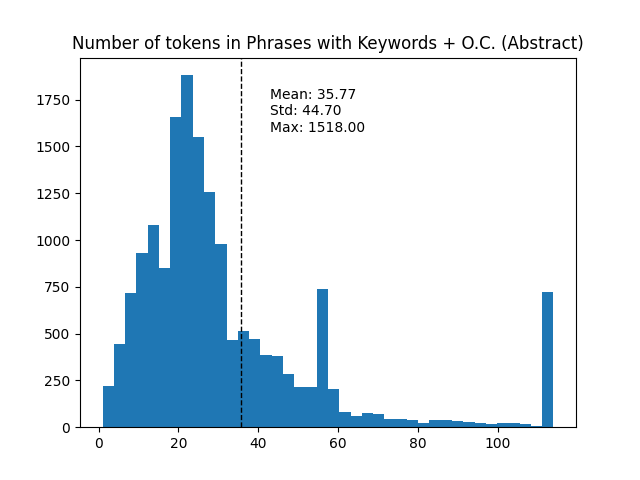
\includegraphics[width=0.45\textwidth]{Figures/05/Histograms/preprocessing length histogram sentence_with_keywords_parsed_trafilatura_abstract_keep_original_content.png}
        \end{adjustbox}
    
        %\label{fig:image1}
    }

    
    \subfigure[\keyphrasesFulltextOnly{}]{

    \begin{adjustbox}{max height=0.18\textheight}
           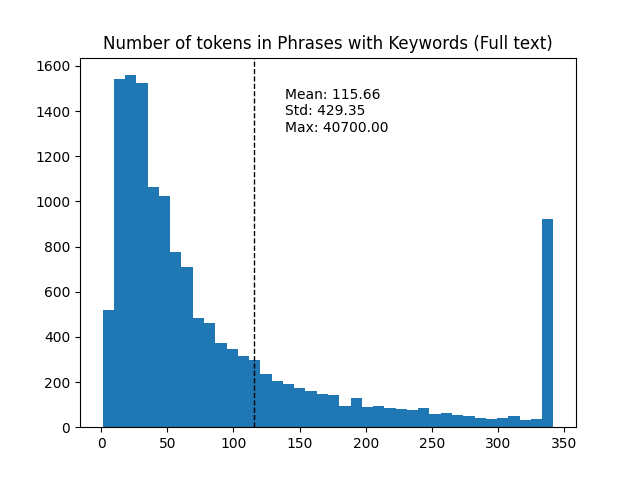
\includegraphics[width=0.45\textwidth]{Figures/05/Histograms/preprocessing length histogram sentence_with_keywords_parsed_trafilatura_fulltext_only_relevant_sentences.png}
        \end{adjustbox}
    
        %\label{fig:image4}
    }
    \hfill
        \subfigure[\keyphrasesFulltextOC{}]{
        \begin{adjustbox}{max height=0.18\textheight}
            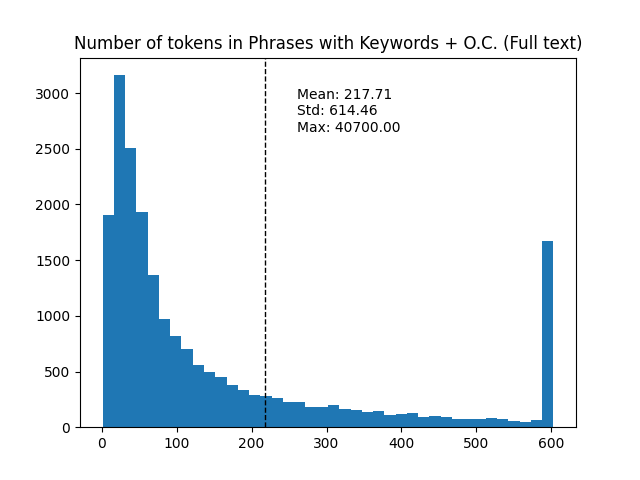
\includegraphics[width=0.45\textwidth]{Figures/05/Histograms/preprocessing length histogram sentence_with_keywords_parsed_trafilatura_fulltext_keep_original_content.png}
        \end{adjustbox}
        
        %\label{fig:image3}
    }

    
    \caption{
    Length (in n. of tokens) of the \contentType{}s in the \VSI{} dataset after preprocessing}
    \label{fig:05_vsi_token_distribution_after_preprocessing}
\end{figure}



\input{Tables/05/Mean_length_comparison}

\putInBox{
By applying our preprocessing approach, we construct eight labelled datasets for binary \textclassification{} (Figure \ref{fig:05_vsi_pos_neg_balance}). These datasets exhibit a balance of positives and negatives ranging from 12 to 14\% positives, and from 86 to 88\% negatives\footnote{For more details, see Table \ref{appendix03:tab:vsi_positive_negative_balance} in \appendixname{} \ref{appendix03:preprocessing_statistics}}, representing a slight improvement compared to the original dataset, which had a balance of 10\% positives to 90\% negatives (Figure \ref{fig:04_naive_positives_and_negatives}). 
}

The only exception are the \keyphrases{} from the \trafilaturaAbstract{} discarding Original Content (``\keyphrasesAbstractOnly{}"). This specific dataset displays a 27\% positive and 73\% negative balance. The reasons behind this imbalance can be attributed to the factors previously explained. As the metadata required for extracting the \trafilaturaAbstract{} may be empty or uninformative; and few entries may contain the exact search keywords we are looking for; the dataset is substantially reduced, resulting in only 4,050 unique entries for the \keyphrasesAbstractOnly{}  as opposed to the original 19,939  unique entries for the \trafilaturaAbstract{} ($\approx$ 20\% left). Consequently, the significantly smaller dataset size has led to a noticeable change in the balance of the labels.


\begin{figure}[ht]
    \centering
    \subfigure[\trafilaturaTitle{}]{
        \begin{adjustbox}{max height=0.18\textheight}
            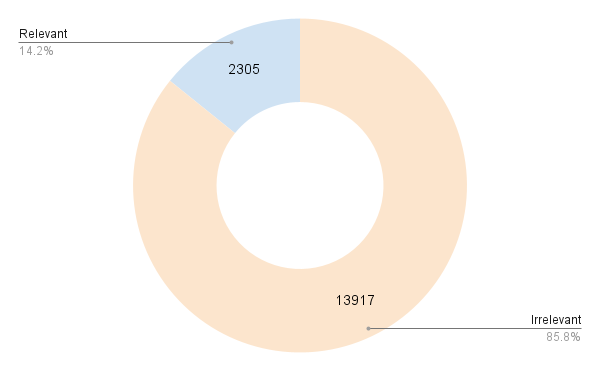
\includegraphics[width=0.45\textwidth]{Figures/05/Charts/balance Title.png}
        \end{adjustbox}
        
        %\label{fig:image1}
    }
    \hfill
    \subfigure[\trafilaturaAbstract{}]{
        \begin{adjustbox}{max height=0.18\textheight}
            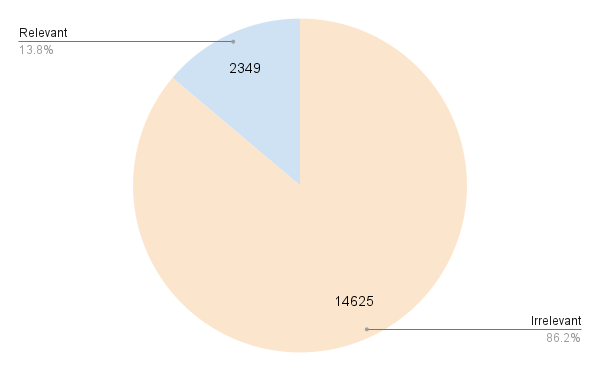
\includegraphics[width=0.45\textwidth]{Figures/05/Charts/balance Abstract.png}
        \end{adjustbox}
        
        %\label{fig:image2}
    }
    
    \subfigure[\trafilaturaFulltext{}]{
        \begin{adjustbox}{max height=0.18\textheight}
            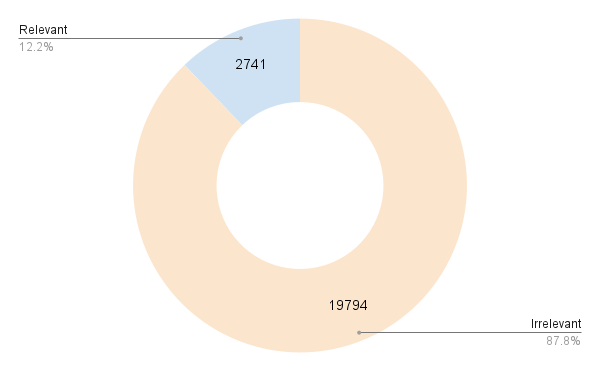
\includegraphics[width=0.45\textwidth]{Figures/05/Charts/balance Fulltext.png}
        \end{adjustbox}
        
        %\label{fig:image3}
    }
    \hfill
    \subfigure[\translationTitle{}]{
        \begin{adjustbox}{max height=0.18\textheight}
            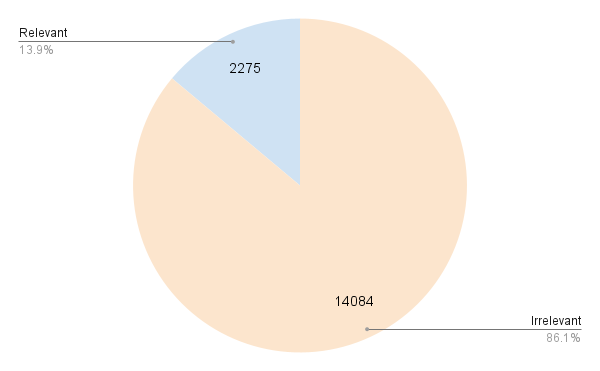
\includegraphics[width=0.45\textwidth]{Figures/05/Charts/balance Translated Title.png}
        \end{adjustbox}
        %\label{fig:image4}
    }
    
    
    %%
    \subfigure[\keyphrasesAbstractOnly{}]{
        \begin{adjustbox}{max height=0.18\textheight}
            \includegraphics[width=0.45\textwidth]{Figures/05/Charts/balance Sentence with Keywords Abstract.png}
        \end{adjustbox}
        %\label{fig:image2}
    }
    \hfill
    \subfigure[\keyphrasesAbstractOC{}]{
        \begin{adjustbox}{max height=0.18\textheight}
            \includegraphics[width=0.45\textwidth]{Figures/05/Charts/balance Sentece with Keywords and OC Abstract.png}
        \end{adjustbox}
        %\label{fig:image1}
    }

    
    \subfigure[\keyphrasesFulltextOnly{}]{
        \begin{adjustbox}{max height=0.18\textheight}
            \includegraphics[width=0.45\textwidth]{Figures/05/Charts/balance Sentence with keywords Fulltext.png}
        \end{adjustbox}
        %\label{fig:image4}
    }
    \hfill
    \subfigure[\keyphrasesFulltextOC{}]{
        \begin{adjustbox}{max height=0.18\textheight}
            \includegraphics[width=0.45\textwidth]{Figures/05/Charts/balance Sentence with keywords and OC Fulltext.png}
        \end{adjustbox}
        %\label{fig:image3}
    }

    
    \caption{Positive/Negative balance after preprocessing the \VSI{} dataset}
    \label{fig:05_vsi_pos_neg_balance}
\end{figure}




% making sure to print all tables and figures 
\clearpage
%\customHeader{1}{Preprocessing the \sanba{} dataset}
\label{sanba_preprocessing}



















% making sure to print all tables and figures 
\clearpage

\customHeader{0}{Methodology}
\label{06_methodology}


\customHeader{1}{BERT Models}
\label{06_bert_models}



As previously mentioned in \headerName{} \ref{02_bert_models_for_text_classification}, the \gls{bert} architecture from \mytextcite{BERT_paper} has been customized for various tasks, resulting in a wide array of models to select from. For our project, we have opted to employ six different \gls{bert} models, based on their specialized task and the characteristics of our data.
%Since our data is multilingual in nature, 
We utilize \gls{bert} models that differentiate between upper case and lower case characters (\texttt{cased} versions). Additionally, due to computational constraints, we opt for the basic (\texttt{base}) versions of the models rather than the \texttt{large} ones (Table \ref{tab:06_bert_sizes}).

\input{Tables/06/06_bert_size_comparison}


\customHeader{2}{\bertbase{}}
\label{06_bert_base}
The original \gls{bert} model developed by Google in \mytextcite{BERT_paper}. It was trained on a large corpus of English text from Wikipedia and Google’s BooksCorpus dataset, using a \gls{wp} tokenizer.

\customHeader{2}{\bertmultilingual{}}
\label{06_bert_multilingual}
The Multilingual \gls{bert} \myparencite{BERT_paper} is a version of the original \gls{bert} model that is designed to handle text in multiple languages. It was trained on the top 104 languages with the biggest Wikipedia sizes by number of articles, using a \gls{wp} tokenizer. 

\customHeader{2}{\bertbiolinkbert{}}
\label{06_bert_biolinkbert}

This model was introduced in \mytextcite{linkbert_biolinkbert} as the result of training a classical \gls{bert} architecture while enriching the context of the documents by using two corpora of documents linked to one another by hyperlinks. For documents $doc_1, doc_2$ linked by a hyperlink $doc_1 \to doc_2$, during the training phase, the sections of $doc_2$ that are reachable by the hyperlink will be concatenated to their corresponding sections from $doc_1$ for the Next Sentence Prediction task (See \headerName{} \ref{02_next_sentence_prediction}). This process increases the context available for the model to learn embeddings. 

The authors present a model for the general domain (Link-BERT), trained on the English Wikipedia with hyperlinks; and a model for the biomedical domain (\bertbiolinkbert{}), trained on PubMed\footnote{\url{https://pubmed.ncbi.nlm.nih.gov/}} abstracts (in English) containing hyperlinks, and used a \gls{wp} tokenizer. As of the culmination of our work, \bertbiolinkbert{} is still one of the top performing \gls{bert} models in the \gls{blurb} \myparencite{blurb_biomedical_ranking}.


\customHeader{2}{\bertscibert{}}
\label{06_bert_scibert}
This model was introduced in \mytextcite{scibert} as a specialized model for scientific texts. It was trained with the classical \gls{bert} architecture using 1.14 million papers in English from Semantic Scholar\footnote{\url{https://www.semanticscholar.org/}}, $82\%$ of which belong to the biomedical domain. The authors use the full text from the papers. 


\customHeader{2}{\bertroberta{}}
\label{06_bert_roberta}

This model was introduced in \mytextcite{roberta} and is an extension and improvement of the original \gls{bert} model. \bertroberta{} follows the same architecture as \gls{bert} but undergoes a more extensive pre-training process, specifically, it uses much larger batch sizes, longer sequences, and removes the Next Sentence Prediction" task used in \gls{bert}. Additionally, it is trained on 10 times more data than \gls{bert}, by merging five datasets: Google’s BooksCorpus, the English Wikipedia, Common-Crawl\footnote{\url{https://commoncrawl.org/}} English News \myparencite{ccnews_dataset}, OpenWebText \myparencite{openwebtext}, and the ``Stories" subset of the Common-Crawl \myparencite{stories_dataset}. It uses a \gls{bpe} tokenizer.

\customHeader{2}{\bertxlmroberta{}}
\label{06_bert_xlmroberta}

This model was introduced in \mytextcite{xlm_roberta} as the multilingual version of \bertroberta{}. For training, the authors constructed the 100-CC corpus for training \bertxlmroberta{}, which consists of monolingual data in 100 languages from the Common-Crawl, and used a SentencePiece tokenizer \myparencite{sentencepiece}, which extends the classical \gls{bpe} tokenization algorithm. 





\customHeader{2}{Excluded Models}
\label{06_bert_excluded_models}

Initially, we considered three other \gls{bert} models; however, after careful consideration, we decided not to include them due to various reasons.



\begin{paragraph}{ChouBERT}
    This model was introduced in
    \mytextcite{choubert} as a specialized model for Plant Health Monitoring. However, it was trained exclusively on French texts, which raises strong concerns about its ability to generalize to our linguistically and thematically diverse dataset.
\end{paragraph}

\begin{paragraph}{DistilBERT}
    This model was introduced in
    \mytextcite{distilbert} as a smaller version of the original \gls{bert} model. It uses a process called ``distillation", which compresses the knowledge of a larger \gls{bert} model into a smaller one, while still retaining decent performance. 

    During our preliminary training experiments with the \gls{bert} models mentioned above, DistilBERT consistently underperformed. Regardless of the configurations used, it defaulted to predicting the majority class. Therefore, we chose to omit DistilBERT from our final model selection.

\end{paragraph}


\begin{paragraph}{BioBERT}
    This model was introduced in \mytextcite{biobert} as a \gls{bert} variant specifically designed for biomedical text and tasks. Once again, this model uses the classical \gls{bert} architecture on PubMed abstracts in English. Since it has been vastly outperformed by \bertbiolinkbert{} in several \gls{nlp} tasks \myparencite{linkbert_biolinkbert}, we decided not to include it in our final model selection.
\end{paragraph}


% choubert
% distilbert
% biobert

\customHeader{1}{Finetuning}
\label{06_finetuning}



\begin{figure}
    \centering
    \includegraphics[width=0.75\textwidth]{Figures/06/06_BERT_for_embeddings.png}
    %\caption{Caption}
    %\label{fig:enter-label}
\end{figure}


\begin{figure}[ht]
    \centering
    \subfigure[\trafilaturaTitle{}]{
        \begin{adjustbox}{max height=0.18\textheight}
            \includegraphics[width=0.45\textwidth]{Figures/06/06_BERT_for_embeddings.png}
        \end{adjustbox}
        
        %\label{fig:image1}
    }
    \hfill
    \subfigure[\trafilaturaAbstract{}]{
        \begin{adjustbox}{max height=0.18\textheight}
            \includegraphics[width=0.45\textwidth]{Figures/06/06_BERT_finetuning.png}
        \end{adjustbox}
        
        %\label{fig:image2}
    }
\end{figure}
\customHeader{1}{Pattern-Exploiting Training}
\label{06_pet}

\clearpage
\customHeader{0}{Results and Discussion}
\label{07_results_and_discussion}


In this section, we present the results of our training experiments, and comment on them.



In this \headerName{}, we present the results of our training experiments, and provide insights on them.


%Due to space constraints, we're unable to display all the metrics from the training data. 
Comprehensive training plots and logs can be found in our GitLab repository. For a glimpse into the results from our initial training round, refer to Figures \ref{fig:07_vsi_sample_training_logs_unbalanced} and \ref{fig:07_vsi_sample_training_logs_pet_1000}. 
In the first figure, we can see that the optimal epoch to avoid overfitting in that particular scenario is the fourth epoch, which coincidentally also maximizes the \fTwo{}. 
In contrast, in the second image, the first epoch is optimal, while it does not have the best \fTwo{}.



\begin{figure}[ht]
    \centering
    \subfigure[Training Loss]{
            \includegraphics[width=0.3\textwidth]{Figures/07/sample_result/unbalanced_mbert_trafilatura_title_loss.png}
    }
    \hfill
    \subfigure[Development Loss]{
            \includegraphics[width=0.3\textwidth]{Figures/07/sample_result/unbalanced_mbert_trafilatura_title_eval_loss.png}
    }
    \hfill
    \subfigure[Development \fTwo{}]{
            \includegraphics[width=0.3\textwidth]{Figures/07/sample_result/unbalanced_mbert_trafilatura_title_eval_f_beta_2.0.png}
    }
    \caption{\unbalanced{} - Losses and Development \fTwo{} evolution for \bertmultilingual{} on the \trafilaturaTitle{}}
    \label{fig:07_vsi_sample_training_logs_unbalanced}
\end{figure}


\begin{figure}[ht]
    \centering
    \subfigure[Training Loss]{
            \includegraphics[width=0.3\textwidth]{Figures/07/sample_result/pet1000_roberta_trafilatura_title_loss.png}
    }
    \hfill
    \subfigure[Development Loss]{
            \includegraphics[width=0.3\textwidth]{Figures/07/sample_result/pet1000_roberta_trafilatura_title_eval_loss.png}
    }
    \hfill
    \subfigure[Development \fTwo{}]{
            \includegraphics[width=0.3\textwidth]{Figures/07/sample_result/pet1000_roberta_trafilatura_title_eval_f_beta_2.0.png}
    }
    \caption{\petThousand{} - Losses and Development \fTwo{} evolution for \bertroberta{} on the \trafilaturaTitle{}}
    \label{fig:07_vsi_sample_training_logs_pet_1000}
\end{figure}



The optimal epochs for each training scenario are detailed in \appendixname{} \ref{appendix05:vsi_optimal_epochs}. It's evident that \unbalanced{} takes the longest to reach the optimal epoch, especially when compared to the other methods, where the majority reach the optimum within the first or second epoch. The disparity between the two fine-tuning techniques is significant, with \balanced{} often reaching its peak performance in just one epoch. When it comes to \gls{pet}, all five scenarios exhibit a consistent pattern, typically achieving their optimal epoch before the fourth one. This suggests that any variations in the rate of convergence might occur during the training of the \gls{pet} ensembles. Given that all ensembles undergo training for five epochs, it must be that this sufficient for achieving satisfactory results. Unfortunately, we did not record the evolution of the custom losses used to train the \gls{pet} ensembles.


\begin{figure}[ht]
    \centering
    \subfigure{
            \includegraphics[width=0.45\textwidth]{Figures/07/mBERT Classifier at optimal epoch_trafilatura.png}
    }
    %\hfill
    \subfigure{
            \includegraphics[width=0.45\textwidth]{Figures/07/mBERT Classifier at optimal epoch_keyphrases.png}
    }
    \caption{Development \fTwo{} for \bertmultilingual{} at the optimal epochs, across all the training methods}
    \label{fig:07_dev_f2_mbert}
\end{figure}

Based on these findings, we moved forward to the second round, trained models up to their optimal epochs, and evaluated their final performance.
The metrics for the best classifiers across each training scenario and for every \gls{bert} model are detailed in \appendixname{} \ref{appendix05:vsi_metrics_optimal_epochs}. 
A direct comparison of the Development \fTwo{} outcomes reveals that \unbalanced{} consistently underperforms compared to other training techniques
\footnote{A \fTwo{} score of 0\% indicates the model defaulted to predict the predominant class (negative)} (See Figure \ref{fig:07_dev_f2_mbert} for sample results for \bertmultilingual{}).
In fact, \balanced{} outperforms \unbalanced{} in nearly all instances, with only one exception\footnote{This specific instance pertains to \bertbase{} on the \trafilaturaTitle{}, showing a marginal difference of about 3\%}.

When examining \gls{pet}, a noticeable trend emerges: performance improves as the document count per category grows. Specifically, the Development \fTwo{} for \petFifty{} generally lags behind other \gls{pet} variants and seldom matches their levels. Conversely, both \petFiveHundred{} and \petThousand{} consistently register superior results.


Given the high number of training scenarios (totaling $336$), we may impose a stringent performance threshold, focusing only on classifiers that achieve a Development \fTwo{} of at least 80\%. 
Out of all the scenarios, only 72 classifiers meet this criterion, which is roughly one-fifth of the total.
A summary of these top-performing classifiers is provided in Table \ref{appendix05:tab:f2_auc_top_pergorming_by_model}. It's evident from the table that \gls{pet} training typically surpasses \finetuning{}\footnote{The sole exception being \bertxlmroberta{} on the \trafilaturaFulltext{}}, and that 
\unbalanced{} never makes it to the list. 
Among the \gls{pet} configurations, both \petFiveHundred{} and \petThousand{} consistently exceed the set threshold.


When ranking the \gls{bert} models based on the number of top-performing classifiers, \bertxlmroberta{} leads with 22, followed closely by \bertmultilingual{} and \bertbiolinkbert{}, each with 16. 
This suggests that the multilingual nature of our dataset might play a more pivotal role in determining relevance than its biomedical aspect. 
This aligns with the fact that only 4 top classifiers are associated with \bertscibert{}, and a mere 3 with \bertbase{}. 
\bertroberta{}, with its 11 top classifiers, occupies a middle ground, possibly indicating its superior capabilities compared to \bertbase{} and \bertscibert{}. However, its training exclusively on English text might be a limiting factor.

At the same time, it's concerning to observe that several top classifiers exhibit worryingly low Development \auc{} values, ranging between 60\% and 80\% (Figure \ref{fig:07_vsi_sample_auc}). 
A low \auc{} indicates challenges faced by these models in differentiating between positive and negative instances. 
Yet, their high \fTwo{} scores suggest a pronounced recall relative to precision. 
Piecing these insights together, it's plausible that these models achieve elevated \fTwo{} scores by predominantly categorizing most documents as positive.


\begin{figure}[ht]
    \centering
    \subfigure[\bertbiolinkbert{} with \petFifty{} on the \trafilaturaTitle{}]{
            \includegraphics[width=0.3\textwidth]{Figures/07/sample_auc/biolinkbert_pet_50_trafilatura_title_dev_ROC_on_split.png}
    }
    \hfill
    \subfigure[\bertroberta{} with \petTwoHundred{} on the \trafilaturaFulltext{}]{
            \includegraphics[width=0.3\textwidth]{Figures/07/sample_auc/roberta_pet_200_trafilatura_fulltext_dev_ROC_on_split.png}
    }
    \hfill
    \subfigure[\bertxlmroberta{} with \petThousand{} on the \trafilaturaFulltext{} ]{
            \includegraphics[width=0.3\textwidth]{Figures/07/sample_auc/xlmroberta_pet_1000_fulltext_dev_ROC_on_split.png}
    }
    \caption{Sample \auc{}s for some classifiers}
    \label{fig:07_vsi_sample_auc}
\end{figure}


Prioritizing models that genuinely grasp the concept of relevance rather than indiscriminately marking everything as positive, we set a threshold of 80\% for the Development \auc{}. By doing so, we narrow down to 49 classifiers, detailed in Table \ref{appendix05:tab:f2_auc_f1_top_pergorming_by_content_type}.
Interestingly, the \contentType{} with the highest number of top-performing classifiers is the \trafilaturaFulltext{}, exhibiting 15 top classifiers across all \gls{bert} models.
This indicates that the \trafilaturaFulltext{}, typically longer than other \contentType{}s, offers ample content, enabling all models to effectively learn the task.

Conversely, it's worth noting that the \keyphrasesAbstractOnly{} doesn't feature on the list. 
As discussed in \headerName{} \ref{vsi_preprocessing}, this dataset undergoes significant reduction during preprocessing, potentially leaving it with insufficient content.
Given that we still have four top-performing classifiers for the \trafilaturaAbstract{}, we opt to \textbf{exclude} the \keyphrasesAbstractOnly{} as a \contentType{}.


To avoid classifiers that flag almost everything as a positive, we impose a 75\% threshold on the Development \fOne{}.
This criterion narrows our selection to 17 classifiers. 
Table \ref{appendix05:tab:metrics_for_best_classifiers} presents the Development and Test metrics for these classifiers, emphasizing the top-performing metrics.
Once more, the \trafilaturaFulltext{} dominates with the most classifiers on this list (9), and its best three metrics are highlighted.

Predictably, the Test metrics are lower than the Development metrics. 
Yet, it's striking to see a significant drop in the \fOne{} and precision, with most falling below the 50\% mark. 
This trend can be attributed to our emphasis on the \fTwo{}, which leans towards Recall at the expense of Precision. At the same time, the highest Test Recalls hover around or exceed 80\%.


Observe that the \keyphrasesFulltextOnly{} is absent from the list. 
This can be attributed to the significant reduction in dataset content when only sentences containing keywords are considered. 
Additionally, the peak metrics for \keyphrasesAbstractOC{} and \keyphrasesFulltextOC{} consistently fall short of those for \trafilaturaAbstract{} and \trafilaturaFulltext{}, respectively.
These findings suggest that incorporating \keyphrases{} as \contentType{}s does \textbf{not} enhance performance, contrary to our hypothesis in \headerName{} \ref{vsi_leveraging_keywords}. 
Consequently, we opt to \textbf{exclude} these sources of content moving forward, and thus, we are left with the four original \contentType{}s.


Considering the best performing classifiers (Table \ref{tab:07_best_classifiers}), it's noteworthy that, except for one, all top classifiers are derived from \petThousand{}.
Moreover, the best classifiers are consistently obtained by training multilingual \gls{bert} models. This highlights the significance of the multilingual nature of our dataset in determining relevance over its biomedical aspect.


\input{Tables/07/best_classifiers}

\putInBox{

In summary, among all the training methods examined in our work, \unbalanced{} yields the least favorable performance, while \gls{pet} demonstrates increasingly improved performance as more documents per category are introduced. In terms of \contentType{}s, incorporating keywords from the documents does not enhance performance, whereas utilizing the \trafilaturaFulltext{} proves to be the most effective in providing substantial content for the models to learn from, with the \trafilaturaTitle{}, \translationTitle{} and \trafilaturaAbstract{} lagging behind. Additionally, the multilingual aspect of our dataset appears to hold greater significance than their biomedical content, as evidenced by the superior performance of classifiers trained with multilingual \gls{bert} models.


}


Finally, we put forward a reason for the enhanced performance of \gls{pet} compared to \finetuning{}. We theorize that the use of task descriptions in \gls{pet} enables the model to have a clearer comprehension of the task. To illustrate this idea, we reference an example from the foundational \gls{pet} paper by \mytextcite{pet_paper}.

Take into account the next three statements: the first two have labels, and our challenge is to assign a label to the third.


\begin{itemize}
    \item[1.] Category A: This \textit{was} the best \textit{pizza} I've ever had.
    \item[2.] Category B: You \textit{can} get better sushi for half the \textit{price}.
    \item[3.] Category ?: \textit{Pizza} \textit{was} average. Not worth the \textit{price}.
\end{itemize}
\vspace{4pt}

Based solely on this data, determining a label is challenging: Is the focus on pizza or price? Or is it about identifying verb tenses (Past vs. Present)? Yet, if we're informed that the objective is to identify sentences discussing pizza, we'd promptly label the third sentence in category A. Conversely, if it's about prices, category B would be the appropriate label. 

For our task, consider the three following (artificial) sentences:
\begin{itemize}
    \item[1.] Relevant: Oriental Fruit fly (Bactrocera dorsalis) detected in a new location in Central Asia.
    \item[2.] Irrelevant: Check out the best decorative plants for your garden this summer, and beware of insects! 
    \item[3.] Category ?: What to do if you find fruit flies plaguing your field - Agriculture News Online. 
\end{itemize}
\vspace{4pt}

For the task of identifying document relevance for Plant Health Surveillance, we categorize the third sentence as 'Irrelevant'. However, such subtleties might be overlooked by a language model without additional context.


Indeed, referring to Table \ref{tab:07_best_classifiers}, it's evident that \finetuning{} yields one of the top classifiers only when applied to the \trafilaturaFulltext{}. 
Throughout our analysis, we've observed that many top-performing classifiers were also trained on the \trafilaturaFulltext{}. 
This suggests that due to its length (averaging 1102 tokens, but cut at 300 input tokens), the \trafilaturaFulltext{} provides ample content, enabling any \gls{bert} model to grasp the task effectively.
In contrast, other \contentType{}s, being much shorter than the \trafilaturaFulltext{}, might not offer sufficient context for the models. For instance, the \trafilaturaTitle{} averages 11 tokens, the \trafilaturaAbstract{} 50 tokens, and the \translationTitle{} 12 tokens. 
As a result, classifiers benefit from the added context given by \gls{pet} patterns.

Furthermore, it's worth noting that all other best classifiers predominantly use \petThousand{}. 
This suggests that exposing the model to more document examples combined with task-specific knowledge enhances its performance.
However, the performance improvement stales over time, as the incremental gains from transitioning from \petFiveHundred{} to \petThousand{} are marginal, as seen in Tables \ref{tab:07_f2_bert_base}-\ref{tab:07_f2_bert_xlmroberta}.

In conclusion, by employing \gls{pet} and its patterns, we inject task-specific knowledge, thereby guiding the model. 


\clearpage
\customHeader{0}{Conclusions}
\label{08_conclusion}

\clearpage

% %%%%%%%%%%%%%%%%%%%%%%%%%%%%%%%%%%%%%%%%%%%%%%%%%%%%%%%%%%%%%%%%%%%%%%%%%%%%%%%%%%%%%%
% appendices
\appendix

\customHeader{0}{\VSI{} Dataset samples and language statistics}
\label{appendix01:vsi_dataset}

This appendix presents tables and statistics to provide a deeper insight into the characteristics of the \VSI{} dataset. 

\customHeader{1}{Keywords for constructing the \VSI{} Database}
\label{appendix01:vsi_keywords}

\input{Tables/04/Keywords_for_google_search}

\clearpage

\customHeader{1}{Sample entries detected as Latin}
\label{appendix01:vsi_latin}


\begin{table}[!htbp]
    \centering
    \resizebox{0.75\textwidth}{!}{
    \begin{tabular}{|l|}
        \hline
        Text \\
        \hline
        %'Onagri Vigilance \\

      \cvtag{Bactrocera (Daculus) oleae} (Gmelin, 1790) \\
       resting on a leaf - \cvtag{\cvtag{Popillia japonica}} \\
       La \cvtag{Popillia japonica} devasta colture in Piemonte \\
       Regione attiva piano anti \cvtag{Popillia japonica} - www.lombardianotizie.online \ldots \\
       \cvtag{Popillia japonica} | Libero Quoditiano.it \\
       Lombardy: anti \cvtag{Popillia japonica} plan activated in Milan – Lombardy \\
       \cvtag{Candidatus liberibacter} 第1页\\
       Milano, area di San Siro: Regione attiva piano anti \cvtag{Popillia japonica} \\
        %"A Salussola è emergenza \cvtag{Popillia japonica}; mai come quest'anno s'era vista una tale invasione | SalussolaNews" \\
       A Milano il piano anti \cvtag{Popillia japonica} | Milano.zone \\
       Vithal \cvtag{Popillia japonica} Polysect Ultra SL PFnPO Le Migliori Venditori \\
       ultime notizie su ore popillia \\
       \cvtag{Meridiem} Seeds presenta Yuparanà nel Lazio \\
       Lombardia: al via piano regionale contro la \cvtag{Popillia japonica} a San Siro (2) \\
       Milano, area di San Siro: Regione attiva piano anti \cvtag{Popillia japonica} \\
       Control of \cvtag{Anthracnose} \ldots by \cvtag{Colletotrichum musae} \ldots\\
       \ldots on \cvtag{Curcuma alismatifolia Gagnep} using \cvtag{Antagonistic Bacillus} spp.\\
       Lombardia: al via piano regionale contro la \cvtag{Popillia japonica} a San Siro \\
       \cvtag{Popillia japonica}, come difendersi \\
       Japankäfer $<$i$>$\cvtag{Popillia japonica}$<$/i$>$ \\
       RETI INSETTICIDE PER \cvtag{Popillia japonica} - Asso Web TV \\
       La \cvtag{Popillia japonica} \\
       \cvtag{Citrus tristeza} virus \ldots of \cvtag{Candidatus Liberibacter Asiaticus} by \cvtag{Diaphorina citri}\\
       \cvtag{Popillia japonica} \\
       \cvtag{Popillia} devastante nel Santhiatese - Prima Vercelli \\
        \hline
    \end{tabular}
    }
    \caption{Sample entries detected as Latin text}
    \label{tab:appendix01:latin_entries}
\end{table}

\clearpage

\customHeader{1}{\VSI{} Language statistics}
\label{appendix01:vsi_language_distribution}


Table \ref{appendix01:tab:language_distribution} shows the distribution of languages (by ISO code) in the \VSI{} dataset as automatically detected by the Google Translate API.


\begin{table}%[!htbp]
\centering
\resizebox{0.55\textwidth}{!}{
\begin{tabular}{lclclc}
\textbf{Language} & \textbf{Entries} & \textbf{Language} & \textbf{Entries} & \textbf{Language} & \textbf{Entries} \\
\hline
af & 18 & id & 226 & ro & 77 \\
am & 2 & ig & 3 & ru & 180 \\
ar & 226 & ilo & 24 & rw & 13 \\
az & 13 & is & 34 & sd & 1 \\
be & 3 & it & 4788 & sk & 66 \\
bg & 107 & iw & 13 & sl & 51 \\
bn & 6 & ja & 74 & sm & 1 \\
bs & 33 & jv & 2 & sn & 8 \\
ca & 142 & jw & 1 & so & 4 \\
ceb & 7 & ka & 13 & sq & 18 \\
co & 121 & kk & 7 & sr & 12 \\
cs & 94 & kn & 4 & su & 1 \\
cy & 5 & ko & 51 & sv & 53 \\
da & 35 & kri & 5 & sw & 14 \\
de & 362 & ku & 3 & ta & 4 \\
el & 164 & ky & 1 & te & 9 \\
en & 12016 & la & 152 & tg & 12 \\
eo & 7 & lb & 28 & th & 31 \\
es & 3025 & ln & 3 & tk & 3 \\
et & 31 & lo & 4 & tl & 3 \\
eu & 3 & lt & 26 & tr & 83 \\
fa & 36 & lv & 11 & ts & 3 \\
fi & 25 & mg & 4 & tt & 1 \\
fil & 11 & mi & 5 & uk & 30 \\
fr & 2251 & mk & 1 & ur & 1 \\
fy & 12 & mo & 8 & uz & 11 \\
ga & 8 & mr & 19 & vi & 210 \\
gd & 3 & ms & 17 & yi & 1 \\
gl & 18 & mt & 6 & yo & 1 \\
gn & 69 & ne & 2 & zh & 41 \\
gu & 6 & nl & 465 & zh-CN & 784 \\
ha & 2 & no & 29 & zh-TW & 72 \\
haw & 3 & ny & 6 & zu & 4 \\
hi & 39 & om & 11 & Failed & 6132 \\
hmn & 2 & pl & 135 & \ & \ \\
hr & 77 & ps & 3 & \ & \ \\
ht & 4 & pt & 1292 & \ & \ \\
hu & 184 & qu & 4 & \ & \ \\
hy & 2 & \ & \ & \ & \ \\
\end{tabular}
}
\caption{Number of entries per language in the \VSI{} Dataset}
\label{appendix01:tab:language_distribution}
\end{table}



\customHeader{0}{Regular expressions used in this project}
\label{appendix02:regular_expressions}

This Appendix contains examples of the regular expressions used for different tasks in this project.


\customHeader{1}{Error Message Removal - \VSI{} Dataset}
\label{appendix02:pesv_error_regex}

\begin{table}[ht]
\centering
\begin{tabular}{|l|}
\hline
\textbf{Regular Expressions} \\ \hline
\verb|^JavaScript is not available\.$| \\
\verb|^Error$| \\
%\verb|^Text$| \\
\verb|^NA$| \\
\verb|^Timeout error$| \\
%\verb|^post_title$| \\
\verb|^None$| \\
%\verb|^Home$| \\
\verb|^Loading(\.)*$| \\
%\verb|^Facebook$| \\
%\verb|^Idioma$| \\
%\verb|^Publications$| \\
%\verb|^Buscar$| \\
%\verb|^Search$| \\
\verb|^Not Found$| \\
\verb|^Access Restricted$| \\
%\verb|^DSpace JSPUI$| \\
\verb|^Page Not Found$| \\
%\verb|^Archives$| \\
%\verb|^Author Details$| \\
\verb|^\[\]$| \\
\verb|^blacklisted| \\
\verb|^'NoneType' object has no attribute 'get'?$| \\
%\verb|^Copyright All Rights Reserved.+$| \\
\verb|^PPlease Wait\.\.\.\s+ Cloudflare$| \\
\verb|^HTTPSConnectionPool.*| \\
%\verb|^HTTPConnectionPool.*| \\
\verb|^Checking your browser.*| \\
%\verb|^Facebook\s+Twitter\s+Instagram$| \\
%\verb|^Sequence Features$| \\
%\verb|^Discover open access scientific publications$| \\
%\verb|^Abbonati subito$| \\
\verb|^Please update your browser$| \\
%\verb|^News$| \\
\verb|^JavaScript n'est pas disponible\.$| \\
\verb|^Vos données\.% Votre expérience\.*$| \\
%\verb|^Related Articles$| \\
\verb|^Before you continue to YouTube$| \\
%\verb|^常用链接$| \\
%\verb|^Google Search Console$| \\
%\verb|^Cultures$| \\
%\verb|^Browse Articles$| \\
%\verb|^Article Versions Notes$| \\
%\verb|^Datasets$| \\
\verb|^Just a moment(\.)*| \\
%\verb|^Search Results$| \\
%\verb|^Browsing by Title$| \\
%\verb|^Search\. Read\. Cite\.$| \\
%\verb|^Agricultura$| \\
%\verb|^datosrevista$| \\
%\verb|^Journal$| \\
\verb|^Your data\. Your experience\.$| \\
%\verb|^Table of Contents$| \\
\verb|^Access Denied$| \\
\ldots \\
\hline
\end{tabular}
\caption{Some Regular Expressions for Removing Errors Messages in the  \VSI{} dataset}
\label{appendix02:tab:error_messages}
\end{table}








\customHeader{1}{Noise Removal - \VSI{} Dataset}
\label{appendix02:pesv_noise_removal}

\begin{landscape}
\begin{table}%[ht]
\resizebox{\paperwidth}{!}{
    \begin{tabular}{|l|p{6.5cm}| p{6cm}|}
\hline
\textbf{Description} & \textbf{Regular Expression} & \textbf{Explanation}\\ \hline
Emojis & \texttt{[\textbackslash U00010000-\textbackslash U0010ffff]} & Unicode emojis\\ \hline

Hyphen-like Characters & \texttt{[\textbackslash u002D\textbackslash u058A\textbackslash u2010\textbackslash u2011\textbackslash u2012} \texttt{\textbackslash u2013\textbackslash u2014\textbackslash u2015\textbackslash u2E3A} \texttt{\textbackslash u2E3B\textbackslash uFE58\textbackslash uFE63\textbackslash uFF0D]} 
&
Common hyphen-like characters in Unicode  such as ֊ ‐ ‑ ‒ – — ⸺ ⸻ ﹘ ﹣ -, etc.
\\ \hline
Quotation-mark-like Characters & \texttt{[\textbackslash u00BB\textbackslash u00AB\textbackslash u25B7\textbackslash u2018\textbackslash u2019} \texttt{\textbackslash u201C\textbackslash u201D\textbackslash u2039\textbackslash u203A} \texttt{\textbackslash u300C\textbackslash u300D\textbackslash u300E\textbackslash u300F} \texttt{\textbackslash u301D\textbackslash u301E\textbackslash u301F\textbackslash uFE41} \texttt{\textbackslash uFE42\textbackslash uFE43\textbackslash uFE44\textbackslash uFF02} \texttt{\textbackslash uFF07\textbackslash uFF62\textbackslash uFF63]} & 
Common quotation-mark-like characters in Unicode, such as » « ▷ ‘ ’ “ ” ‹ › 「 」『 』〝 〞 〟 ﹁ ﹂ ﹃ ﹄ " ' 「 」
\\ \hline
URL & \texttt{\textbackslash bhttps?://\textbackslash S+\textbackslash b} & \\ \hline
Date & \texttt{\textbackslash b\d\{4\}[.-/]\d\{1,2\}[.-/]\d\{1,2\}\textbackslash b|\textbackslash b\d\{1,2\}[.-/]\d\{1,2\}[.-/]\d\{4\}\textbackslash b|\textbackslash b\d\{1,2\}[.-/]\d\{1,2\}[.-/]\d\{1,2\}\textbackslash b}   
&
Date pattern for dates in formats YYYY-MM-DD, DD-MM-YYYY, DD.MM.YYYY, DD/MM/YYY, etc....
\\ \hline
Hours & \texttt{\textbackslash b\d\{1,2\}:\d\{2\}(?::\d\{2\})?\textbackslash b} 
& 
Hours pattern e.g. 10:30 AM, 15:45, or 2023-05-15 10:30:00. Also, 15:45:30 and 2023-05-15T12:30:45+00:00, etc
\\
\hline

    \end{tabular}
}
\caption{Regular Expressions for Noise Removal}
\label{appendix02:tab:pesv_string_cleaning_regex}
\end{table}
\end{landscape}

\newpage



\cleardoublepage
\newpage
\bibliographystyle{unsrt}
%\bibliography{erreferentziak}
\bibliography{References/references}
%% ALDATU HEMEN EDUKIEN ZERRENDAN AGERTUKO DEN 
\addcontentsline{tof}{chapter}{\bibname}


\cleardoublepage
\newpage
\appendix
%\appendix

\customHeader{0}{\VSI{} Dataset samples and language statistics}
\label{appendix01:vsi_dataset}

This appendix presents tables and statistics to provide a deeper insight into the characteristics of the \VSI{} dataset. 

\customHeader{1}{Keywords for constructing the \VSI{} Database}
\label{appendix01:vsi_keywords}


\begin{table}%[]
    \centering
    %\begin{tabular}{|p|p|p|}
    \resizebox{\textwidth}{!}{
    \begin{tabular}{|p{0.3\textwidth}|c|p{0.4\textwidth}|}
    \hline
    \textbf{Organism of interest} &\textbf{Type of organism} & \textbf{Search Query} \\
    \hline
    
     Fusarium oxysporum f. sp. cubense tropical (race 4) &  Fungus &\cvtag{fusarium oxysporum tropical}  \\
     % https://en.wikipedia.org/wiki/Fusarium_oxysporum_f.sp._cubense#Tropical_Race_4/TR4
     Xylella fastidiosa & Bacteril & \cvtag{xylella}  \\
     % https://en.wikipedia.org/wiki/Xylella_fastidiosa
     Bursaphelenchus xylophilus &  Nematode & \cvtag{Bursaphelenchus xylophilus} \\
     % https://en.wikipedia.org/wiki/Bursaphelenchus_xylophilus
     Bactrocera dorsalis & Insect &  \cvtag{Bactrocera dorsalis} \\
     % https://en.wikipedia.org/wiki/Bactrocera_dorsalis
     Candidatus Liberibacter spp. &  Bacteria & \cvtag{huanglongbing} \\
     % https://en.wikipedia.org/wiki/Liberibacter
     Popillia japonica & Insect & \cvtag{Popillia Japonica} \\
     % https://en.wikipedia.org/wiki/Japanese_beetle
     Flavescence dor\'ee &  Bacteria  &  \cvtag{flavescence} \\
     % https://en.wikipedia.org/wiki/Flavescence_dor%C3%A9e
     Tomato brown rugose fruit virus &  Virus & \cvtag{ToBRFV}\\
     % https://en.wikipedia.org/wiki/Tomato_brown_rugose_fruit_virus
     Spodoptera frugiperda & Insect & \cvtag{spodoptera frugiperda} \\
     % https://en.wikipedia.org/wiki/Fall_armyworm
     Bretziella fagacearum & Fungus & \cvtag{oak wilt Bretziella} \\
     % https://wiki.pestinfo.org/wiki/Bretziella_fagacearum
     Agrilus planipennis & Insect & \cvtag{Agrilus planipennis}  \\
     % https://en.wikipedia.org/wiki/Emerald_ash_borer
     Thaumatotibia leucotreta & Insect &  \cvtag{Thaumatotibia leucotreta} \\
     % https://en.wikipedia.org/wiki/False_codling_moth
     Xylotrechus chinensis & Insect & \cvtag{Xylotrechus chinensis}  \\
     % https://es.wikipedia.org/wiki/Xylotrechus_chinensis
     Toumeyella parvicornis & Insect & \cvtag{Toumeyella parvicornis}  \\
     % https://en.wikipedia.org/wiki/Toumeyella_parvicornis
     Ceratocystis platani & Fungus &  \cvtag{Ceratocystis platani}  \cvtag{chancre du platane}  \\ \hline
     % https://en.wikipedia.org/wiki/Ceratocystis_platani
     General Plant Health & \  &\cvtag{first report plant disease} \cvtag{new plant health}   \\
    \hline
    \end{tabular}
    }
    \caption{Keywords and key phrases used for the \VSI dataset}
    \label{tab:04_query_keywords}
\end{table}


\clearpage

\customHeader{1}{Sample entries detected as Latin}
\label{appendix01:vsi_latin}


\begin{table}[!htbp]
    \centering
    \resizebox{0.75\textwidth}{!}{
    \begin{tabular}{|l|}
        \hline
        Text \\
        \hline
        %'Onagri Vigilance \\

      \cvtag{Bactrocera (Daculus) oleae} (Gmelin, 1790) \\
       resting on a leaf - \cvtag{\cvtag{Popillia japonica}} \\
       La \cvtag{Popillia japonica} devasta colture in Piemonte \\
       Regione attiva piano anti \cvtag{Popillia japonica} - www.lombardianotizie.online \ldots \\
       \cvtag{Popillia japonica} | Libero Quoditiano.it \\
       Lombardy: anti \cvtag{Popillia japonica} plan activated in Milan – Lombardy \\
       \cvtag{Candidatus liberibacter} 第1页\\
       Milano, area di San Siro: Regione attiva piano anti \cvtag{Popillia japonica} \\
        %"A Salussola è emergenza \cvtag{Popillia japonica}; mai come quest'anno s'era vista una tale invasione | SalussolaNews" \\
       A Milano il piano anti \cvtag{Popillia japonica} | Milano.zone \\
       Vithal \cvtag{Popillia japonica} Polysect Ultra SL PFnPO Le Migliori Venditori \\
       ultime notizie su ore popillia \\
       \cvtag{Meridiem} Seeds presenta Yuparanà nel Lazio \\
       Lombardia: al via piano regionale contro la \cvtag{Popillia japonica} a San Siro (2) \\
       Milano, area di San Siro: Regione attiva piano anti \cvtag{Popillia japonica} \\
       Control of \cvtag{Anthracnose} \ldots by \cvtag{Colletotrichum musae} \ldots\\
       \ldots on \cvtag{Curcuma alismatifolia Gagnep} using \cvtag{Antagonistic Bacillus} spp.\\
       Lombardia: al via piano regionale contro la \cvtag{Popillia japonica} a San Siro \\
       \cvtag{Popillia japonica}, come difendersi \\
       Japankäfer $<$i$>$\cvtag{Popillia japonica}$<$/i$>$ \\
       RETI INSETTICIDE PER \cvtag{Popillia japonica} - Asso Web TV \\
       La \cvtag{Popillia japonica} \\
       \cvtag{Citrus tristeza} virus \ldots of \cvtag{Candidatus Liberibacter Asiaticus} by \cvtag{Diaphorina citri}\\
       \cvtag{Popillia japonica} \\
       \cvtag{Popillia} devastante nel Santhiatese - Prima Vercelli \\
        \hline
    \end{tabular}
    }
    \caption{Sample entries detected as Latin text}
    \label{tab:appendix01:latin_entries}
\end{table}

\clearpage

\customHeader{1}{\VSI{} Language statistics}
\label{appendix01:vsi_language_distribution}


Table \ref{appendix01:tab:language_distribution} shows the distribution of languages (by ISO code) in the \VSI{} dataset as automatically detected by the Google Translate API.


\begin{table}%[!htbp]
\centering
\resizebox{0.55\textwidth}{!}{
\begin{tabular}{lclclc}
\textbf{Language} & \textbf{Entries} & \textbf{Language} & \textbf{Entries} & \textbf{Language} & \textbf{Entries} \\
\hline
af & 18 & id & 226 & ro & 77 \\
am & 2 & ig & 3 & ru & 180 \\
ar & 226 & ilo & 24 & rw & 13 \\
az & 13 & is & 34 & sd & 1 \\
be & 3 & it & 4788 & sk & 66 \\
bg & 107 & iw & 13 & sl & 51 \\
bn & 6 & ja & 74 & sm & 1 \\
bs & 33 & jv & 2 & sn & 8 \\
ca & 142 & jw & 1 & so & 4 \\
ceb & 7 & ka & 13 & sq & 18 \\
co & 121 & kk & 7 & sr & 12 \\
cs & 94 & kn & 4 & su & 1 \\
cy & 5 & ko & 51 & sv & 53 \\
da & 35 & kri & 5 & sw & 14 \\
de & 362 & ku & 3 & ta & 4 \\
el & 164 & ky & 1 & te & 9 \\
en & 12016 & la & 152 & tg & 12 \\
eo & 7 & lb & 28 & th & 31 \\
es & 3025 & ln & 3 & tk & 3 \\
et & 31 & lo & 4 & tl & 3 \\
eu & 3 & lt & 26 & tr & 83 \\
fa & 36 & lv & 11 & ts & 3 \\
fi & 25 & mg & 4 & tt & 1 \\
fil & 11 & mi & 5 & uk & 30 \\
fr & 2251 & mk & 1 & ur & 1 \\
fy & 12 & mo & 8 & uz & 11 \\
ga & 8 & mr & 19 & vi & 210 \\
gd & 3 & ms & 17 & yi & 1 \\
gl & 18 & mt & 6 & yo & 1 \\
gn & 69 & ne & 2 & zh & 41 \\
gu & 6 & nl & 465 & zh-CN & 784 \\
ha & 2 & no & 29 & zh-TW & 72 \\
haw & 3 & ny & 6 & zu & 4 \\
hi & 39 & om & 11 & Failed & 6132 \\
hmn & 2 & pl & 135 & \ & \ \\
hr & 77 & ps & 3 & \ & \ \\
ht & 4 & pt & 1292 & \ & \ \\
hu & 184 & qu & 4 & \ & \ \\
hy & 2 & \ & \ & \ & \ \\
\end{tabular}
}
\caption{Number of entries per language in the \VSI{} Dataset}
\label{appendix01:tab:language_distribution}
\end{table}



\customHeader{0}{Regular expressions used in this project}
\label{appendix02:regular_expressions}

This Appendix contains examples of the regular expressions used for different tasks in this project.


\customHeader{1}{Error Message Removal - \VSI{} Dataset}
\label{appendix02:pesv_error_regex}

\begin{table}[ht]
\centering
\begin{tabular}{|l|}
\hline
\textbf{Regular Expressions} \\ \hline
\verb|^JavaScript is not available\.$| \\
\verb|^Error$| \\
%\verb|^Text$| \\
\verb|^NA$| \\
\verb|^Timeout error$| \\
%\verb|^post_title$| \\
\verb|^None$| \\
%\verb|^Home$| \\
\verb|^Loading(\.)*$| \\
%\verb|^Facebook$| \\
%\verb|^Idioma$| \\
%\verb|^Publications$| \\
%\verb|^Buscar$| \\
%\verb|^Search$| \\
\verb|^Not Found$| \\
\verb|^Access Restricted$| \\
%\verb|^DSpace JSPUI$| \\
\verb|^Page Not Found$| \\
%\verb|^Archives$| \\
%\verb|^Author Details$| \\
\verb|^\[\]$| \\
\verb|^blacklisted| \\
\verb|^'NoneType' object has no attribute 'get'?$| \\
%\verb|^Copyright All Rights Reserved.+$| \\
\verb|^PPlease Wait\.\.\.\s+ Cloudflare$| \\
\verb|^HTTPSConnectionPool.*| \\
%\verb|^HTTPConnectionPool.*| \\
\verb|^Checking your browser.*| \\
%\verb|^Facebook\s+Twitter\s+Instagram$| \\
%\verb|^Sequence Features$| \\
%\verb|^Discover open access scientific publications$| \\
%\verb|^Abbonati subito$| \\
\verb|^Please update your browser$| \\
%\verb|^News$| \\
\verb|^JavaScript n'est pas disponible\.$| \\
\verb|^Vos données\.% Votre expérience\.*$| \\
%\verb|^Related Articles$| \\
\verb|^Before you continue to YouTube$| \\
%\verb|^常用链接$| \\
%\verb|^Google Search Console$| \\
%\verb|^Cultures$| \\
%\verb|^Browse Articles$| \\
%\verb|^Article Versions Notes$| \\
%\verb|^Datasets$| \\
\verb|^Just a moment(\.)*| \\
%\verb|^Search Results$| \\
%\verb|^Browsing by Title$| \\
%\verb|^Search\. Read\. Cite\.$| \\
%\verb|^Agricultura$| \\
%\verb|^datosrevista$| \\
%\verb|^Journal$| \\
\verb|^Your data\. Your experience\.$| \\
%\verb|^Table of Contents$| \\
\verb|^Access Denied$| \\
\ldots \\
\hline
\end{tabular}
\caption{Some Regular Expressions for Removing Errors Messages in the  \VSI{} dataset}
\label{appendix02:tab:error_messages}
\end{table}








\customHeader{1}{Noise Removal - \VSI{} Dataset}
\label{appendix02:pesv_noise_removal}

\begin{landscape}
\begin{table}%[ht]
\resizebox{\paperwidth}{!}{
    \begin{tabular}{|l|p{6.5cm}| p{6cm}|}
\hline
\textbf{Description} & \textbf{Regular Expression} & \textbf{Explanation}\\ \hline
Emojis & \texttt{[\textbackslash U00010000-\textbackslash U0010ffff]} & Unicode emojis\\ \hline

Hyphen-like Characters & \texttt{[\textbackslash u002D\textbackslash u058A\textbackslash u2010\textbackslash u2011\textbackslash u2012} \texttt{\textbackslash u2013\textbackslash u2014\textbackslash u2015\textbackslash u2E3A} \texttt{\textbackslash u2E3B\textbackslash uFE58\textbackslash uFE63\textbackslash uFF0D]} 
&
Common hyphen-like characters in Unicode  such as ֊ ‐ ‑ ‒ – — ⸺ ⸻ ﹘ ﹣ -, etc.
\\ \hline
Quotation-mark-like Characters & \texttt{[\textbackslash u00BB\textbackslash u00AB\textbackslash u25B7\textbackslash u2018\textbackslash u2019} \texttt{\textbackslash u201C\textbackslash u201D\textbackslash u2039\textbackslash u203A} \texttt{\textbackslash u300C\textbackslash u300D\textbackslash u300E\textbackslash u300F} \texttt{\textbackslash u301D\textbackslash u301E\textbackslash u301F\textbackslash uFE41} \texttt{\textbackslash uFE42\textbackslash uFE43\textbackslash uFE44\textbackslash uFF02} \texttt{\textbackslash uFF07\textbackslash uFF62\textbackslash uFF63]} & 
Common quotation-mark-like characters in Unicode, such as » « ▷ ‘ ’ “ ” ‹ › 「 」『 』〝 〞 〟 ﹁ ﹂ ﹃ ﹄ " ' 「 」
\\ \hline
URL & \texttt{\textbackslash bhttps?://\textbackslash S+\textbackslash b} & \\ \hline
Date & \texttt{\textbackslash b\d\{4\}[.-/]\d\{1,2\}[.-/]\d\{1,2\}\textbackslash b|\textbackslash b\d\{1,2\}[.-/]\d\{1,2\}[.-/]\d\{4\}\textbackslash b|\textbackslash b\d\{1,2\}[.-/]\d\{1,2\}[.-/]\d\{1,2\}\textbackslash b}   
&
Date pattern for dates in formats YYYY-MM-DD, DD-MM-YYYY, DD.MM.YYYY, DD/MM/YYY, etc....
\\ \hline
Hours & \texttt{\textbackslash b\d\{1,2\}:\d\{2\}(?::\d\{2\})?\textbackslash b} 
& 
Hours pattern e.g. 10:30 AM, 15:45, or 2023-05-15 10:30:00. Also, 15:45:30 and 2023-05-15T12:30:45+00:00, etc
\\
\hline

    \end{tabular}
}
\caption{Regular Expressions for Noise Removal}
\label{appendix02:tab:pesv_string_cleaning_regex}
\end{table}
\end{landscape}

\newpage




\end{document}